\documentclass{BigNote}

\usetikzlibrary{arrows.meta}
\usetikzlibrary{calc}

\title{大笔记}
\author{我}

\addbibresource{BigNote.bib}
\usepackage{imakeidx}
\makeindex[columns=3, title=名词索引]

\begin{document}
    \maketitle

    \tableofcontents
    \newpage

    \chapter*{前言}
    
    此笔记意在记录学习中的一些命题证明以及想法.

    \chapter{基础知识}
    \section{逻辑}

断言 (statement) 是一类有明确真值 (T/F) 的语句, 我们定义如下运算:

\begin{definition}
    对于断言 \(A\) 定义其否定 (negation) 为 \(\neg A\), 满足如下真值表.
    \begin{center}
        \begin{tabular}{|c|c|}
            \hline
            \(A\) & \(\neg A\) \\
            \hline
            T & F \\
            \hline
            F & T \\
            \hline
        \end{tabular}
    \end{center}

    对于断言 \(A, B\) 定义其合取 (conjuction) 为 \(A \land B\), 其析取 (disjuction) 为 \(A \lor B\), 满足如下真值表.

    \begin{center}
        \begin{tabular}{|c|c|c|c|c|}
            \hline
            \(A\) & \(B\) & \(A \land B\) & \(A \lor B\) \\
            \hline
            T & T & T & T \\
            \hline
            T & F & F & T \\
            \hline
            F & T & F & T \\
            \hline
            F & F & F & F \\
            \hline
        \end{tabular}
    \end{center}
\end{definition}

\begin{definition}
    如果 \(E(x)\) 在 \(x\) 是某些对象时为断言, 则称 \(E(x)\) 为一个性质 (property).
\end{definition}

我们承认类 (class) 的概念如下, 若对象 \(x\) 属于类 \(A\), 则记为 \(x \in A\), 否则记为 \(x \notin A\).
我们用 \(\{x \in X; E(x)\}\) 表示 \(X\) 中所有满足性质 \(E\) 的对象组成的类.

\begin{definition}
    我们用 \(\exists\) 代表存在某个对象, 用 \(\forall\) 代表所有对象都满足某个性质.

    我们也用 \(\exists !\) 代表存在唯一一个对象.

    我们用 \(a := b\) 标记 \(a\) 由 \(b\) 定义, \(a = b\) 代表 \(a, b\) 仅仅是相同对象的两个表示 (集合论下会重新定义等于).
\end{definition}

我们有如下自明的公式.

\begin{theorem}
    \begin{align}
        \neg \neg A &:= \neg (\neg A) = A \\
        \neg (A \land B) &= \neg A \lor \neg B \\
        \neg (A \lor B) &= \neg A \land \neg B \\
        \neg (\forall x \in X : E(x)) &= \exists x \in X : \neg E(x) \\
        \neg (\exists x \in X : E(x)) &= \forall x \in X : \neg E(x) \\
        \neg (\forall x \in X : (\exists y \in Y : E(x, y))) &= \exists x \in X : (\forall y \in Y : \neg E(x, y)) \\
        \neg (\exists x \in X : (\forall y \in Y : E(x, y))) &= \forall x \in X : (\exists y \in Y : \neg E(x, y))
    \end{align}
\end{theorem}

\begin{definition}
    对于断言 \(A, B\), 我们记断言 \(A\) 能推出 \(B\) 为 \(A \implies B\), 代表
    \begin{equation}
        A \implies B := (\neg A) \lor B
    \end{equation}

    而断言 \(A, B\) 等价 (\(A \iff B\)) 意味着 \((A \implies B) \land (B \implies A)\).
\end{definition}

\begin{theorem}
    我们可以验证下述断言:
    \begin{align}
        (A \implies B) &\iff (\neg B \implies \neg A) \\
        (A \implies B) \land (B \implies C) &\implies (A \implies C)
    \end{align}
\end{theorem}

    \section{初等集合论}

朴素集合论认为

\begin{axiom}
    对于任意性质 \(P\) 均有 \(Y = \{x : P(x)\}\) 为集合.
\end{axiom}

然而随后提出的 Russell 悖论 (Russell's paradox) 给出了性质 \(X: X \notin X\) 对应的的集合不存在, 人们开始探索公理化集合论的道路. 

\subsection{von Neumann-Bernays-Gödel 公理}

von Neumann-Bernays-Gödel 公理系统的核心是类 (class) 与元素 (element), \(A\) 是 \(B\) 的元素用符号 \(A \in B\) 标记,
其否定自然使用 \(\notin\) 标记, 一个类可以作为另一个类的元素.

\begin{definition}
    两个类 \(A\) 与 \(B\) 相等, 记作 \(A = B\), 当且仅当 \(A\) 与 \(B\) 有相同的元素, 其否定记为 \(A \neq B\).

    \[
        (X = Y) := \forall Z (Z \in X \iff Z \in Y)
    \]
\end{definition}

\begin{corollary}
    显见以下公式:

    \begin{enumerate}
        \item \(\forall X (X = X)\)
        \item \(\forall X \forall Y (X = Y \implies Y = X)\)
        \item \(\forall X \forall Y \forall Z ((X = Y \land Y = Z) \implies X = Z)\)
    \end{enumerate}
\end{corollary}

\begin{definition}
    一个类 \(A\) 是另一个类 \(B\) 的子类, 记作 \(A \subseteq B\), 当且仅当 \(A\) 的所有元素都是 \(B\) 的元素, 其否定记为 \(A \nsubseteq B\).

    \[
        (X \subseteq Y) := \forall Z (Z \in X \implies Z \in Y)
    \]

    我们用 \(A \subset B\) 表示 \(A \subseteq B \land A \neq B\), 称非空 \(A \subset B\) 为真子类.
\end{definition}

\begin{corollary}
    \[
        (X \subseteq Y) \land (Y \subseteq X) \iff (X = Y)
    \]
\end{corollary}

\begin{axiom}[Axiom of Equality]
    \setlabel {Axiom of Equality}
    \label {axiom:NBG Axiom of Equality}
    \[
        \forall X \forall Y (X = Y \implies \forall Z (X \in Z \iff Y \in Z))
    \]
\end{axiom}

\begin{definition}[集合]
    一个类 \(X\) 称集合 (set), 当且仅当 \(\exists Y (X \in Y)\), 本节中我们用小写字母 \(x, y, z, \dots\) 表示集合, 用大写字母 \(X, Y, Z, \dots\) 表示类.
\end{definition}

\begin{definition}[真类]
    一个类 \(X\) 称真类 (proper class), 当且仅当 \(X\) 不是集合, 常用粗体字母 \(\mathbf{X}, \mathbf{Y}, \mathbf{Z}, \dots\) 表示真类.
\end{definition}

\begin{axiom}[Axiom of Pair]
    \setlabel {Axiom of Pair}
    \label {axiom:NBG Axiom of Pair}
    \[
        \forall x \forall y \exists z \forall u (u \in z \iff (u = x \lor u = y))
    \]
\end{axiom}

上述公理展开可得 \(\forall x \forall y ((\exists X \exists Y (x \in X \land y \in Y)) \implies \exists z \exists Z (z \in Z \land \forall u (u \in Z \iff (u = x \lor u = y))))\),
记集合 \(z = \{x,y\}\), 特别的, 当 \(x = y\) 时, 我们记 \(z = \{x\}\).

为了方便叙述, 我们常常忽略公式最前的 \(\forall\)

\begin{corollary}
    显见以下公式:

    \begin{enumerate}
        \item \(((x = u \land y = v) \implies \{x,y\} = \{u,v\})\)
        \item \(\{x,y\} = \{y,x\}\).
        \item \(x = y \iff \{x\} = \{y\}\).
        \item \(x = y \iff \forall Z (x \in Z \iff y \in Z)\).
    \end{enumerate}
\end{corollary}

\begin{definition}[有序对]
    \label {definition:Kuratowski ordered pair}
    有序对 (ordered pair) \((x,y)\) 定义为 \(\{\{x\},\{x,y\}\}\).
\end{definition}

\begin{lemma}
    有序对的有序体现在其性质 \((x,y) = (u,v) \iff (x = u \land y = v)\).

    \begin{proof}
        \((\impliedby)\) 显然.

        \((\implies)\) 若 \(x \neq u\), 则 \(\{x\} \neq \{u\}\), 依赖 \ref{axiom:NBG Axiom of Pair}
        \(\{x\} \in (x,y) = (u,v)\), 从而 \(u \in \{u, v\} = \{x\}\), 矛盾.

        若 \(x = u \land y \neq v\), 只需证明 \(a = b \iff \{c,a\} = \{c,b\}\), 
        由 \ref{axiom:NBG Axiom of Pair} 知 \(a \in \{c,a\} = \{c,b\}\) 从而 \(a = c\), 同理, 
        \(b = c\), 矛盾.
    \end{proof}
\end{lemma}

\begin{definition}[有序三元对]
    \label {definition:ordered triple}
    有序三元对 (ordered triple) \((x,y,z)\) 定义为有序对 \(((x,y),z)\).
\end{definition}

\begin{definition}[二元关系]
    \label {definition:binary relation}
    类 \(R\) 称二元关系 (binary relation), 当且仅当 \(R\) 是有序对的集合, 记作 \(\mathbf{isbinrel} (R)\).

    \[
        \mathbf{isbinrel} (R) \iff \forall z (z \in R \implies \exists x \exists y (z = (x,y)))
    \]
\end{definition}

在不久的将来, 我们将用二元关系定义映射.

\begin{axiom}[Axiom of Membership]
    \setlabel {Axiom of Membership}
    \label {axiom:NBG Axiom of Membership}
    \[
        \exists \mathfrak{E} \forall z (z \in \mathfrak{E} \iff \exists x \exists y (z = (x,y) \land x \in y))
    \]
\end{axiom}

\begin{axiom}[Axiom of Domain]
    \setlabel {Axiom of Domain}
    \label {axiom:NBG Axiom of Domain}
    \[
        \forall X \exists D \forall x (x \in D \iff \exists y ((x,y) \in X))
    \]
\end{axiom}

\begin{definition}
    \label {definition:domain}
    上述定义中类 \(D\) 称为 \(X\) 的定义域 (domain), 记作 \(\mathbf{dom} (X)\).
\end{definition}

\begin{definition}
    \label {definition:universe}
    定义 \(\mathfrak{U} := \mathbf{dom} (\mathfrak{E})\), 称为宇宙 (universe), 注意到 \(\forall x (x \in \{x\})\),
    从而 \(\forall x (x \in \mathfrak{U})\).
\end{definition}

\begin{corollary}
    \[
        \mathbf{dom} (\mathfrak{U}) = \mathfrak{U}
    \]
\end{corollary}

\begin{axiom}[Axiom of Difference]
    \setlabel {Axiom of Difference}
    \label {axiom:NBG Axiom of Difference}
    \[
        \forall X \forall Y \exists D \forall x (x \in D \iff (x \in X \land x \notin Y))
    \]
\end{axiom}

\begin{definition}
    \label {definition:difference of two classes}
    上述定义中类 \(D\) 称为 \(X\) 与 \(Y\) 的差集 (difference), 记作 \(X \setminus Y\).
\end{definition}

\begin{definition}
    \label {definition:intersection of two classes}
    定义 \(X \cap Y := X \setminus (X \setminus Y)\), 称为 \(X\) 与 \(Y\) 的交集 (intersection).
\end{definition}

\begin{definition}
    \label {definition:union of two classes}
    定义 \(X \cup Y := \mathfrak{U} \setminus ((\mathfrak{U} \setminus X) \cap (\mathfrak{U} \setminus Y))\), 称为 \(X\) 与 \(Y\) 的并集 (union).
\end{definition}

\begin{definition}
    \label {definition:symmetric difference of two classes}
    定义 \(X \triangle Y := (X \setminus Y) \cup (Y \setminus X)\), 称为 \(X\) 与 \(Y\) 的对称差 (symmetric difference).
\end{definition}

\begin{definition}
    \label {definition:empty class}
    定义 \(\varnothing := \mathfrak{U} \setminus \mathfrak{U}\), 称为空类 (empty class), 根据 \ref{axiom:ZF Axiom of Infinity} 空类是集合 (空集, empty set).
\end{definition}

\begin{corollary}
    \[
        \forall E (\varnothing = E \setminus E)
    \]

    \begin{proof}
        运用 \ref{axiom:NBG Axiom of Equality} 即可.
    \end{proof}
\end{corollary}

\begin{axiom}[Axiom of Product]
    \setlabel {Axiom of Product}
    \label {axiom:NBG Axiom of Product}
    \[
        \forall X \forall Y \exists P \forall z (z \in P \iff \exists x \exists y (z = (x,y) \land x \in X \land y \in Y))
    \]
\end{axiom}

\begin{definition}
    \label {definition:product of two classes}
    上述定义中类 \(P\) 称为 \(X\) 与 \(Y\) 的积 (product), 记作 \(X \times Y\).
\end{definition}

\begin{definition}
    定义宇宙的积 \(\mathfrak{U} \times \mathfrak{U} := \ddot {\mathfrak{U}}\),
    此时 \(\mathbf{isbinrel} (R) \iff R \subseteq \ddot {\mathfrak{U}}\).
\end{definition}

\begin{axiom}[Axiom of Inversion]
    \setlabel {Axiom of Inversion}
    \label {axiom:NBG Axiom of Inversion}
    \[
        \forall X \exists I \forall z (z \in I \iff \exists x \exists y (z = (x,y) \land (y,x) \in X))
    \]
\end{axiom}

\begin{axiom}[Axiom of Cycle]
    \setlabel {Axiom of Cycle}
    \label {axiom:NBG Axiom of Cycle}
    \[
        \forall X \exists C \forall t (t \in C \iff \exists x \exists y \exists z (t = (z,x,y) \land (x,y,z) \in X))
    \]
\end{axiom}

\begin{definition}
    由上述公理定义的 \(I\) 记作 \(X^{-1}\), 称为 \(X\) 的逆 (inverse), \(C\) 记作 \(X^{\circlearrowright}\), \(X^{\circlearrowleft} := {(X^{\circlearrowright})}^{\circlearrowright}\).
\end{definition}

\begin{definition}
    \label {definition:range}
    定义 \(\mathbf{ran} (X) := \mathbf{dom} (X^{-1})\), 称为 \(X\) 的值域 (range).
\end{definition}

\begin{definition}
    \label{definition:union of classes}
    定义类 \(X\) 的并 (union) \(\bigcup X := \{z : \exists y \in X (z \in y)\}\).
    \label{definition:intersection of classes}
    定义类 \(X\) 的交 (intersection) \(\bigcap X := \{z : \forall y \in X (z \in y)\}\).
    \label{definition:power class}
    定义类 \(X\) 的幂 (power) \(\mathcal{P} (X) := \{Y : Y \subseteq X\}\).

    这里用到对类的表示方法, \(\{x : \phi (x)\}\) 表示满足条件 \(\phi (x)\) 的所有元素的类.

    \begin{proof}
        存在性依次由以下三者给出:

        \[
            \bigcup X = \mathbf{dom} (\mathfrak{E} \cap (\mathfrak{U} \times X))
        \]

        \[
            \bigcap X = \mathfrak{U} \setminus \mathbf{dom} ((\ddot {\mathfrak{U}} \setminus \mathfrak{E}) \cap (\mathfrak{U} \times X))
        \]

        \[
            \mathcal{P} (X) = \mathfrak{U} \setminus \mathbf{dom} (\mathfrak{E}^{-1} \cap (\mathfrak{U} \times (\mathfrak{U} \setminus X)))
        \]
    \end{proof}
\end{definition}

\begin{corollary}
    \[
        \mathcal{P} (\mathfrak{U}) = \mathfrak{U}
    \]
\end{corollary}

\begin{definition}
    \label {definition:image of a class}
    给出类 \(X\) 与二元关系 \(R\), 定义 \(X\) 在 \(R\) 下的像 (image) \(R[X] := \{y : \exists x \in X ((x,y) \in R)\} = \mathbf{ran} [R \cap (X \times \mathfrak{U})]\).

    \label {definition:preimage of a class}
    同理定义其逆像 (preimage) \(R^{-1}[X]\).
\end{definition}

\begin{definition}
    \label {definition:composition of two classes}
    给出二元关系 \(F, G\), 定义 \(F\) 与 \(G\) 的复合 (composition) \(F \circ G := \{(x,z) : \exists y ((x,y) \in G \land (y,z) \in F)\}\).

    \begin{proof}
        \[
            F \circ G = \mathbf{dom} ({(G^{-1} \times \mathfrak{U})}^{\circlearrowleft} \cup {(F^{-1} \times \mathfrak{U})}^{\circlearrowright})
        \]
    \end{proof}
\end{definition}

\begin{definition}
    \label {definition:function (set)}
    映射 (function) \(f\) 定义为满足 \((x,y) \in f \land (x,y^\prime) \in f \implies y = y^\prime\) 的二元关系, 记作 \(\mathbf{isfunc} (f)\).

    在存在 \(y\) 的情况下我们记 \(f(x)\) 为唯一的 \(y\) 使得 \((x,y) \in f\), 称为 \(f\) 在 \(x\) 处的值 (value), 映射有时也称函数.
\end{definition}

\begin{definition}
    \label {definition:injective (set)}
    单射 (injective) 指代 \(f, f^{-1}\) 都是映射的二元关系 \(f\).
\end{definition}

\begin{corollary}
    给出映射 \(F, G\), \(F \circ G\) 也是映射.
\end{corollary}

接下来从类转向集合, 定义集合的操作与要求.

\begin{axiom}[Axiom of Replacement]
    \setlabel {Axiom of Replacement}
    \label {axiom:NBG Axiom of Replacement}
    \[
        \forall x \forall F (\mathbf{isfunc} (F) \implies \exists y (y = F[x]))
    \]
\end{axiom}

\begin{axiom}[Axiom of Union]
    \setlabel {Axiom of Union}
    \label {axiom:NBG Axiom of Union}
    \[
        \forall x \exists y (y = \bigcup x)
    \]
\end{axiom}

\begin{axiom}[Axiom of Power Set]
    \setlabel {Axiom of Power Set}
    \label {axiom:NBG Axiom of Power Set}
    \[
        \forall x \exists y (y = \mathcal{P} (x))
    \]
\end{axiom}

\begin{axiom}[Axiom of Infinity]
    \setlabel {Axiom of Infinity}
    \label {axiom:NBG Axiom of Infinity} (存在归纳集)
    \[
        \exists x (\varnothing \in x \land \forall y (y \in x \implies y \cup \{y\} \in x))
    \]
\end{axiom}

\begin{axiom}[Axiom of Foundation]
    \setlabel {Axiom of Foundation}
    \label {axiom:NBG Axiom of Foundation}
    \[
        \forall x (x \neq \varnothing \implies \exists y (y \in x \land y \cap x = \varnothing))
    \]
\end{axiom}

\begin{axiom}[Axiom of Global Choice]
    \setlabel {Axiom of Global Choice}
    \label {axiom:NBG Axiom of Global Choice}
    \[
        \exists f (\mathbf{isfunc} (f) \land \forall x (x \neq \varnothing \implies \exists y (y \in x \land (x,y) \in f)))
    \]
\end{axiom}

上述 \ref{axiom:NBG Axiom of Global Choice} 有个弱化版本如下:

\begin{axiom}[Axiom of Choice]
    \setlabel {Axiom of Choice}
    \label {axiom:NBG Axiom of Choice}
    \[
        \forall x \exists f (\mathbf{isfunc} (f) \land \forall y ((y \in x \land y \neq \varnothing) \implies \exists z ((y,z) \in f \land z \in y)))
    \]
\end{axiom}

称满足上述定理要求的映射 \(f\) 为 \(x\) 上的选择函数 (choice function).

NBG 公理 \cite{TarasBanakh:ClassicalSetTheory} 由以下 14 条公理组成:

\begin{enumerate}
    \item \ref{axiom:NBG Axiom of Equality}
    \[
        \forall X \forall Y (X = Y \implies \forall Z (X \in Z \iff Y \in Z))
    \]
    \item \ref{axiom:NBG Axiom of Pair}
    \[
        \forall x \forall y \exists z \forall u (u \in z \iff (u = x \lor u = y))
    \]
    \item \ref{axiom:NBG Axiom of Membership}
    \[
        \exists \mathfrak{E} \forall z (z \in \mathfrak{E} \iff \exists x \exists y (z = (x,y) \land x \in y))
    \]
    \item \ref{axiom:NBG Axiom of Domain}
    \[
        \forall X \exists D \forall x (x \in D \iff \exists y ((x,y) \in X))
    \]
    \item \ref{axiom:NBG Axiom of Difference}
    \[
        \forall X \forall Y \exists D \forall x (x \in D \iff (x \in X \land x \notin Y))
    \]
    \item \ref{axiom:NBG Axiom of Product}
    \[
        \forall X \forall Y \exists P \forall z (z \in P \iff \exists x \exists y (z = (x,y) \land x \in X \land y \in Y))
    \]
    \item \ref{axiom:NBG Axiom of Inversion}
    \[
        \forall X \exists I \forall z (z \in I \iff \exists x \exists y (z = (x,y) \land (y,x) \in X))
    \]
    \item \ref{axiom:NBG Axiom of Cycle}
    \[
        \forall X \exists C \forall t (t \in C \iff \exists x \exists y \exists z (t = (z,x,y) \land (x,y,z) \in X))
    \]
    \item \ref{axiom:NBG Axiom of Replacement}
    \[
        \forall x \forall F (\mathbf{isfunc} (F) \implies \exists y (y = F[x]))
    \]
    \item \ref{axiom:NBG Axiom of Union}
    \[
        \forall x \exists y (y = \bigcup x)
    \]
    \item \ref{axiom:NBG Axiom of Power Set}
    \[
        \forall x \exists y (y = \mathcal{P} (x))
    \]
    \item \ref{axiom:NBG Axiom of Infinity}
    \[
        \exists x (\varnothing \in x \land \forall y (y \in x \implies y \cup \{y\} \in x))
    \]
    \item \ref{axiom:NBG Axiom of Foundation}
    \[
        \forall x (x \neq \varnothing \implies \exists y (y \in x \land y \cap x = \varnothing))
    \]
    \item \ref{axiom:NBG Axiom of Global Choice}
    \[
        \exists f (\mathbf{isfunc} (f) \land \forall x (x \neq \varnothing \implies \exists y (y \in x \land (x,y) \in f)))
    \]
\end{enumerate}

我们借由 NBG 公理给出一些推论:

\begin{corollary}
    \label {corollary:no infinite descending chain}
    不存在无限降链 (infinite descending chain) \(x_0 \supset x_1 \supset x_2 \supset \dots\), 且不存在 \(x \in x\).

    \begin{proof}
        由 \ref{axiom:NBG Axiom of Foundation}.
    \end{proof}
\end{corollary}

\begin{corollary}
    \label {corollary:NBG every set can be separated by a class}
    集合的子集是集合, 从而集合 \(x\) 与类 \(C\) 的交 \(x \cap C\) 也是集合.

    这里的做法在于使用 \ref{axiom:NBG Axiom of Power Set} 并且意识到 \(y \subseteq x \implies y \in \mathcal{P} (x)\).
\end{corollary}

\begin{corollary}
    \label {corollary:NBG every property can be written as a class}
    我们说明如何把任何一个性质都写作类, 从而我们可以对一个集合进行分离操作, 也即我们给出类 \(\{x : \phi(x,p_1,p_2 \cdots p_n)\}\).

    \begin{proof}
        我们总是将 \(\forall x\) 认作 \(\neg \exists x\), 我们给出一种归纳方法,
        假定公式中有 \(n\) 个变元, 考察 \(\mathfrak{Un} := \mathfrak{U} \times \mathfrak{U} \times \dots \times \mathfrak{U}\) 上的类,
        并且已经将一部分的命题转为类 \(P\), 命题的否定无非是 \(\mathfrak{Un} \setminus P\), 命题的析取无非是 \(P_1 \cap P_2\),
        命题的合取无非是 \(P_1 \cup P_2\), 两个类属于引导出将 \(\mathfrak{E} \times \mathfrak{U} \times \mathfrak{U} \dots \mathfrak{U}\) 上多次施以
        \ref{axiom:NBG Axiom of Cycle} 与 \ref{axiom:NBG Axiom of Inversion} 的结果, 利用 \ref{axiom:NBG Axiom of Domain} 可以丢弃用完的变量.
        从而我们可以将任何命题转为类, 于是可以有集合 \(\{z \in x : P(z)\}\).
    \end{proof}
\end{corollary}

另外的, 将 NBG 公理中的 \ref{axiom:NBG Axiom of Membership}, \ref{axiom:NBG Axiom of Domain},
\ref{axiom:NBG Axiom of Difference}, \ref{axiom:NBG Axiom of Product}, \ref{axiom:NBG Axiom of Inversion},
\ref{axiom:NBG Axiom of Cycle} 替换为以下公理, 我们得到了 BGC 公理, 其与 NBG 等价:

\begin{axiom}[Axiom of Comprehension]
    \setlabel {Axiom of Comprehension}
    \label {axiom:BG Axiom of Comprehension}
    \[
        \forall X_1 \forall X_2 \dots \forall X_n \exists Y (Y = \{x : \phi (x,X_1,X_2, \dots,X_n)\})
    \]
\end{axiom}

更细致的讨论见本章末尾.

\subsection{基本构造}

\begin{corollary}
    集合的子类是集合.

    \begin{proof}
        对 \(X \subseteq y\) 有 \(X \in \mathcal{P} (y)\).
    \end{proof}
\end{corollary}

\begin{definition}
    \label {definition:union of two sets}
    集合 \(x\) 与 \(y\) 的并定义为 \(x \cup y := \bigcup \{x,y\}\).
\end{definition}

\begin{definition}
    \label {definition:intersection of two sets}
    集合 \(x\) 与 \(y\) 的交 \(x \cap y\) 也是集合.

    \begin{proof}
        根据 \ref{corollary:NBG every set can be separated by a class}.
    \end{proof}
\end{definition}

\begin{definition}
    \label {definition:difference of two sets}
    集合 \(x\) 与 \(y\) 的差集 \(x \setminus y\) 是一个集合.

    \begin{proof}
        对 \(x, \mathfrak{U} \setminus y\) 应用 \ref{corollary:NBG every set can be separated by a class}.
    \end{proof}
\end{definition}

\begin{definition}
    \label {definition:product of two sets}
    集合 \(x\) 与 \(y\) 的积 \(x \times y\) 是一个集合.

    \begin{proof}
        \(x \times y \subseteq \mathcal{P} \mathcal{P} (x \cup y)\), 从而是一个集合.
    \end{proof}
\end{definition}

\begin{definition}
    \label {definition:function from a set to a set}
    集合 \(x\) 到 \(y\) 的全体映射 \(y^x\) 构成一个集合.

    \begin{proof}
        \(f \subseteq x \times y\), 从而是一个集合.
    \end{proof}
\end{definition}

\begin{definition}
    \label {definition:surjective (set)}
    对于 \(x,y\) 与 \(f : x \to y\), \(f\) 是满射 (surjective), 当且仅当 \(f[x] = y\).
\end{definition}

\begin{definition}
    存在类 \(\mathfrak{Rel} := \{r : \mathbf{isbinrel} (r)\}\) 为全体二元关系集构成的类.

    \begin{proof}
        \[
            \mathfrak{Rel} = \mathfrak{U} \setminus \mathbf{dom} ((\mathfrak{E}^{-1} \setminus \mathfrak{U} \times (\mathfrak{U} \times \mathfrak{U})))
        \]
    \end{proof}
\end{definition}

以下证明写起来过于冗长, 读者可自行运用 \ref{theorem:Gödel class existence} 进行验证.

\begin{definition}
    存在类 \(\mathfrak{Func} := \{f : \mathbf{isfunc} (f)\}\) 为全体映射集构成的类.
\end{definition}

\begin{definition}
    对于类 \(A,X\) 亦定义 \(X^A\) 为 \(A\) 到 \(X\) 的全体映射构成的类.
\end{definition}

\begin{definition}
    对一个 \(X \subseteq A \times \mathfrak{U}\), 可以视作一组以 \(A\) 为指标的集合 \({(X_\alpha)}_{\alpha \in A}\).
    定义 \(\bigcup_{\alpha \in A} X_\alpha = \mathbf{ran} (X)\), \(\bigcap_{\alpha \in A} X_\alpha = \mathbf{dom} (X)\).

    也可以视作多值函数 (multifunction) \(X : A \multimap \mathfrak{U}\) 给 \(\alpha \in A\) 值 \(X[\{\alpha\}]\),
    并且对 \(B \subseteq A\) 给出 \(X[B] = \mathbf{ran} (X \cap (B \times \mathfrak{U}))\).
\end{definition}

\begin{definition}[笛卡尔积]
    \label {definition:cartesian product}
    对于类 \(A,X \subseteq A \times \mathfrak{U}\), 定义 \(\prod_{\alpha \in A} X_\alpha := \{f \in \mathfrak{Func} : \forall (\alpha \in A)(f(\alpha) \in X_\alpha) \land (\mathbf{dom} (f) = A)\}\), 称为 \(X = (X_\alpha)_{\alpha \in A}\) 的笛卡尔积 (cartesian product).
\end{definition}

真类 \(A\) 诱导出的笛卡尔积是空类.

\begin{definition}[无交并]
    \label {definition:disjoint union}
    对于类 \(A,X \subseteq A \times \mathfrak{U}\), 定义 \(\coprod_{\alpha \in A} X_\alpha := \{(x,y) \in \mathfrak{U} \times A : x \in X_y\}\), 称为 \(X = (X_\alpha)_{\alpha \in A}\) 的无交并 (disjoint union).
\end{definition}

\subsection{Zermelo-Fraenkel 公理}

与 NBG 公理思路不同的是 ZF 公理, ZF 公理体系没有 NBG 公理中类的概念, 或者说 ZF 公理体系中的类 \(C\) 代
指一个有单个自由变量的命题 \(x \in C := \phi(x, p_1, p_2 \dots)\), 其中 \(p_1, p_2 \dots\) 是给定参数.

相应的, 类的运算被视作逻辑命题的计算.

\begin{definition}
    \label {definition:ZF universe}
    定义 \(\mathfrak{U} := \{x : x = x\}\), 称为宇宙 (universe).
    \label {definition:ZF subclass}
    定义 \(X \subseteq Y := \forall x (x \in X \implies x \in Y)\), 称为 \(X\) 是 \(Y\) 的子类 (subclass).
    \label {definition:ZF class intersection}
    定义 \(\bigcap X := \{x : \forall y \in X (x \in y)\}\), 称为 \(X\) 的交集 (intersection).
    \label {definition:ZF class union}
    定义 \(\bigcup X := \{x : \exists y \in X (x \in y)\}\), 称为 \(X\) 的并集 (union).
    \label {definition:ZF power class}
    定义 \(\mathcal{P} (X) := \{Y : Y \subseteq X\}\), 称为 \(X\) 的幂 (power).
    \label {definition:ZF class difference}
    定义 \(X \setminus Y := \{x : x \in X \land x \notin Y\}\), 称为 \(X\) 与 \(Y\) 的差集 (difference).
\end{definition}

此意义上, 集合自然是类 \(\{x:x \in S\}\), ZF 公理包含 (本节大写字母亦表示集合):

\begin{axiom}[Axiom of Extensionality]
    \setlabel {ZFC Axiom of Extensionality}
    \label {axiom:ZF Axiom of Extensionality}
    \[
        \forall X \forall Y (\forall z (z \in X \iff z \in Y) \implies X = Y)
    \]
\end{axiom}

\begin{axiom}[Axiom of Pair]
    \setlabel {ZFC Axiom of Pair}
    \label {axiom:ZF Axiom of Pair}
    \[
        \forall X \forall Y \exists Z \forall U (U \in Z \iff (U = X \lor U = Y))
    \]
\end{axiom}

\begin{axiom}[Axiom of Union]
    \setlabel {ZFC Axiom of Union}
    \label {axiom:ZF Axiom of Union}
    \[
        \forall X \exists Y \forall z (z \in Y \iff \exists u \in X (z \in u))
    \]
\end{axiom}

\begin{axiom}[Axiom of Power Set]
    \setlabel {ZFC Axiom of Power Set}
    \label {axiom:ZF Axiom of Power Set}
    \[
        \forall X \exists Y \forall z (z \in Y \iff z \subseteq X)
    \]
\end{axiom}

\begin{axiom}[Axiom Schema of Separations]
    \setlabel {ZFC Axiom Schema of Separations}
    \label {axiom:ZF Axiom Schema of Separations}
    \[
        \forall X \exists Y \forall z (z \in Y \iff (z \in X \land \phi (z)))
    \]
\end{axiom}

寻此几条公理, 我们仍然可以仿照 NBG 公理进行一些定义, 不过我们要给一个集合作为基础:

\begin{definition}
    \label {definition:ZF empty set}
    空集 (empty set) 定义为 \(\varnothing := \{x \in X : x \neq x\}\), 此中要求至少存在一个集合.

    \label {definition:ZF ordered pair}
    有序对 (ordered pair) \((x,y)\) 定义为 \(\{\{x\},\{x,y\}\}\).

    \label {definition:ZF ordered triple}
    有序三元对 (ordered triple) \((x,y,z)\) 定义为 \(((x,y),z)\).

    \label {definition:ZF set product}
    集合 \(X\) 与 \(Y\) 的积 (product) 定义为 \(X \times Y := \{(x,y) : x \in X \land y \in Y\}\),
    可以由 \(\mathcal{P} (\mathcal{P} (X \cup Y))\) 上用分离公理给出.

    \label {definition:ZF binary relation}
    \(X\) 上的二元关系 (binary relation) 定义为 \(R \subseteq X \times X\).

    \label {definition:ZF function}
    映射 (function) 定义为一个有序对构成的类 \(f\), 且满足
    \(\forall x \forall y \forall z (((x,y) \in f \land (x,z) \in f) \implies (y = z))\).

    映射自然延拓至类, 定义为满足以上唯一性条件且每个元素都是有序对的类.

    \label {definition:ZF image}
    \(X\) 在 \(f\) 下的像 (image) 定义为 \(f[X] := \{y : \exists x \in X ((x,y) \in f)\}\).
\end{definition}

\begin{axiom}[Axiom of Infinity]
    \setlabel {ZFC Axiom of Infinity}
    \label {axiom:ZF Axiom of Infinity}
    \[
        \exists x (\varnothing \in x \land \forall y (y \in x \implies y \cup \{y\} \in x))
    \]
\end{axiom}

\begin{axiom}[Axiom Schema of Replacement]
    \setlabel {ZFC Axiom Schema of Replacement}
    \label {axiom:ZF Axiom Schema of Replacement}
    \[
        \forall f \forall x (\mathbf{isfunc} (f) \implies \exists y (y = f[x]))
    \]
\end{axiom}

\begin{axiom}[Axiom of Regularity]
    \setlabel {ZFC Axiom of Regularity}
    \label {axiom:ZF Axiom of Regularity}
    \[
        \forall x (x \neq \varnothing \implies \exists y (y \in x \land y \cap x = \varnothing))
    \]
\end{axiom}

ZF 公理 \cite{ThomasJech:SetTheory} 代指以下 8 条公理:

\begin{enumerate}
    \item \ref{axiom:ZF Axiom of Extensionality}
    \[
        \forall X \forall Y (\forall z (z \in X \iff z \in Y) \implies X = Y)
    \]
    \item \ref{axiom:ZF Axiom of Pair}
    \[
        \forall X \forall Y \exists Z \forall U (U \in Z \iff (U = X \lor U = Y))
    \]
    \item \ref{axiom:ZF Axiom of Union}
    \[
        \forall X \exists Y \forall z (z \in Y \iff \exists u \in X (z \in u))
    \]
    \item \ref{axiom:ZF Axiom of Power Set}
    \[
        \forall X \exists Y \forall z (z \in Y \iff z \subseteq X)
    \]
    \item \ref{axiom:ZF Axiom Schema of Separations}
    \[
        \forall X \exists Y \forall z (z \in Y \iff (z \in X \land \phi (z)))
    \]
    \item \ref{axiom:ZF Axiom of Infinity}
    \[
        \exists x (\varnothing \in x \land \forall y (y \in x \implies y \cup \{y\} \in x))
    \]
    \item \ref{axiom:ZF Axiom Schema of Replacement}
    \[
        \forall f \forall x (\mathbf{isfunc} (f) \implies \exists y (y = f[x]))
    \]
    \item \ref{axiom:ZF Axiom of Regularity}
    \[
        \forall x (x \neq \varnothing \implies \exists y (y \in x \land y \cap x = \varnothing))
    \]
\end{enumerate}

囊括以下选择公理的体系称为 ZFC 公理:

\begin{axiom}[Axiom of Choice]
    \setlabel {ZFC Axiom of Choice}
    \label {axiom:ZF Axiom of Choice}
    \[
        \forall x \exists f (\mathbf{isfunc} (f) \land \forall y (y \in x \implies \exists z ((y,z) \in f)))
    \]
\end{axiom}

可以发现, NBG 公理中对类操作的 \ref{axiom:NBG Axiom of Equality}, \ref{axiom:NBG Axiom of Membership},
\ref{axiom:NBG Axiom of Domain}, \ref{axiom:NBG Axiom of Difference}, \ref{axiom:NBG Axiom of Product},
\ref{axiom:NBG Axiom of Inversion}, \ref{axiom:NBG Axiom of Cycle}, 在 ZFC 下体现为类背后的逻辑命题的计算,
而 \ref{axiom:NBG Axiom of Pair}, \ref{axiom:NBG Axiom of Union}, \ref{axiom:NBG Axiom of Power Set},
\ref{axiom:NBG Axiom of Infinity}, \ref{axiom:NBG Axiom of Foundation}, \ref{axiom:NBG Axiom of Choice}
在 ZFC 下体现为集合的操作与要求.

可以证明在只考虑集合的情况下, ZFC 公理与 NBG 公理等价, 我们将选取 NBG 公理, 因为一定程度上 NBG 公理表述更加方便, 严格给出了 "类" 的概念, 而非 ZFC 公理中的一个 "语法糖".

\subsection{序数}

序数几乎是集合论上唯一的结构, 有必要对其进行研究.

\subsubsection{偏序}

\begin{definition}
    一个等价关系 \(\sim\) 是满足自反性 (reflexivity), 对称性 (symmetry), 传递性 (transitivity) 的二元关系.
    \begin{enumerate}
        \item 自反性 (reflexivity): \(x \sim x\).
        \item 对称性 (symmetry): \(x \sim y \implies y \sim x\).
        \item 传递性 (transitivity): \(x \sim y \land y \sim z \implies x \sim z\).
    \end{enumerate}


    等价关系给出了集合的一个划分, 也即对于定义于 \(X\) 上的等价关系 \(R \subseteq X \times X\), \(x \in X\) 的等价类 (equivalence class) 定义为

    \begin{equation}
        [x]_R := \{y \in X : x R y\}
    \end{equation}

    对 \(X\) 给出了拆分 \(A = \{S \in \mathcal{P} X : \exists x (S = [x]_R)\}\),
    而 \(X = \bigcup A\) 且 \(\forall S, T \in A : S \cap T = \varnothing \iff S \neq T\).

    同理, 对于一个划分 \(A\), 我们可以定义相应的等价关系 \(R\) 为 \(x R y \iff \exists S \in A (x \in S \land y \in S)\).
\end{definition}



\begin{definition}
    一个二元关系 \(\le\) 称偏序关系 (partial ordering) 若满足:

    \begin{enumerate}
        \item 自反性 (reflexivity): \(x \le x\).
        \item 反对称性 (antisymmetry): \(x \le y \land y \le x \implies x = y\).
        \item 传递性 (transitivity): \(x \le y \land y \le z \implies x \le z\).
    \end{enumerate}

    在只考虑集合 \(P\) 对情况下, 我们也称 \(\le\) 为 \(P\) 上的偏序, 代指 \((\le) \subseteq P \times P\).

    称 \(P\) 上线序则要求 \(\forall x \forall y (x \le y \lor y \le x)\).

    若偏序由 \(\le\) 给定, 我们也用 \(\ge, <, >\), 其意义是自明的.
\end{definition}

\begin{definition}
    对于偏序集 (partially ordered set) \((P, \le)\), 对于 \(X \subseteq P\) 定义:
    \begin{enumerate}
        \item 极大元 (maximal element): \(x \in X\) 为极大元, 若 \(\forall y \in X (x \le y \implies x = y)\).
        \item 极小元 (minimal element): \(x \in X\) 为极小元, 若 \(\forall y \in X (y \le x \implies x = y)\).
        \item 最大元 (greatest element): \(x \in X\) 为最大元, 若 \(\forall y \in X (y \le x)\).
        \item 最小元 (least element): \(x \in X\) 为最小元, 若 \(\forall y \in X (x \le y)\).
        \item 上界 (upper bound): \(x \in X\) 为上界, 若 \(\forall y \in X (y \le x)\).
        \item 下界 (lower bound): \(x \in X\) 为下界, 若 \(\forall y \in X (x \le y)\).
        \item 上确界 (supremum): \(x \in P\) 为上确界, 若 \(x\) 为上界且对于任意上界 \(y\) 有 \(x \le y\).
        \item 下确界 (infimum): \(x \in P\) 为下确界, 若 \(x\) 为下界且对于任意下界 \(y\) 有 \(y \le x\).
    \end{enumerate}
\end{definition}

\begin{definition}
    若偏序集 \((P, \le)\) 中任意两个元素均有上确界和下确界, 命之为格 (lattice), 格的理论将在后面几章叙述.
\end{definition}

\begin{definition}
    偏序是集合上的结构, 我们研究保持偏序结构的映射, 也即对于偏序集 \((P, \le)\) 和 \((Q, \le)\),
    若单射 \(f : P \to Q\) 满足 \(x \le y \implies f(x) \le f(y)\), 则称 \(f\) 为保序映射 (order-preserving map)
    线序间的保序映射也称增 (increasing).
\end{definition}

\begin{definition}
    对于偏序集 \((P, \le_P)\) 和 \((Q, \le_Q)\), 若存在保序双射 \(f : P \to Q\), 且其逆映射亦保序, 则称同构 (isomorphism), 记作 \(P \cong Q\).
\end{definition}

\subsubsection{良序}

\begin{definition}
    一个线序称为良序 (well-ordering), 若其任意非空类均有最小元.
\end{definition}

\begin{lemma}
    \label{lemma:well-ordering increasing map lemma}
    对于良序集 \((W, \le)\) 以及增映射 \(f : W \to W\), 则 \(\forall x (x \le f(x))\).

    \begin{proof}
        构造 \(W\) 子集 \(S = \{x \in W : x > f(x)\}\), \(S\) 有最小元 \(x\),
        而 \(x > f(x)\) 意味着 \(f(x) > f(f(x))\), 而 \(f(x) < x\) 与 \(x\) 最小矛盾.
    \end{proof}
\end{lemma}

\begin{corollary}
    良序集自同构 (automorphism) 必为恒等映射.
\end{corollary}

\begin{corollary}
    两个良序集间的同构存在则唯一.
\end{corollary}

\begin{definition}
    良序集的前段 (initial segment) 定义为 \(S \subseteq W\) 且 \(x \ge y \implies (x \in S \implies y \in S)\).
\end{definition}

\begin{lemma}
    \label{lemma:well-ordering segment is well-ordering lemma}
    前段是良序集, 序继承自原良序集, 并可写成 \(\{x \in W : x < u\}\) 的形式, 称为 \(u\) 的前段 \(W(u)\).

    \begin{proof}
        对于 \(S\) 子集, 取其在 \(W\) 中最小元 \(x\) 即可. 而 \(S\) 可以被写成 \(W \setminus S\) 最小元的前段.
    \end{proof}
\end{lemma}

\begin{lemma}
    \label{lemma:well-ordering segment unequal lemma}
    真前段必不同构于原良序集.

    \begin{proof}
        同构于前段违反 \ref{lemma:well-ordering increasing map lemma}.
    \end{proof}
\end{lemma}

\begin{theorem}
    \label{theorem:well-ordering segment equal theorem}
    任意两个良序集 \(W, W^\prime\) 一下三者成立其一:
    \begin{enumerate}
        \item \(W \cong W^\prime\).
        \item \(W\) 同构于 \(W^\prime\) 的真前段.
        \item \(W^\prime\) 同构于 \(W\) 的真前段.
    \end{enumerate}

    \begin{proof}
        构造 \(f = \{(x,y) \in W \times W^\prime : W(x) \cong W^\prime(y)\}\),
        根据 \ref{lemma:well-ordering segment unequal lemma} 有 \(\{(x,y) \in f \land (x,z) \in f \implies y = z\}\) 与
        \(\{(y,x) \in f \land (z,x) \in f \implies y=z\}\), 
        故 \(f\) 为 \(\mathbf{dom} (f)\) 与 \(\mathbf{ran} (f)\) 间的双射.

        注意到若 \(\mathbf{dom} (f) \neq W\), 且 \(\mathbf{ran} (f) \neq W^\prime\),
        则取最小元 \(x \in W \setminus \mathbf{dom} (f)\) 与 \(y \in W^\prime \setminus \mathbf{ran} (f)\),
        \(f\) 是 \(W(x)\) 与 \(W^\prime(y)\) 间同构故 \((x,y) \in f\), 与 \(x \in \mathbf{dom} (f)\) 矛盾.

        故 \((\mathbf{dom} (f) = W) \land (\mathbf{ran} (f) = W^\prime)\), \((\mathbf{dom} (f) = W) \land \neg(\mathbf{ran} (f) = W^\prime)\), 
        \(\neg(\mathbf{dom} (f) = W) \land (\mathbf{ran} (f) = W^\prime)\) 三者成立其一, 也即上述命题成立.
    \end{proof}
\end{theorem}

\begin{definition}
    同构的良序集称为有同样的序形 (order type), 序数是表示序形的集合.
\end{definition}

\subsubsection{序数}

\begin{definition}
    一个传递集 (transitive set) 定义为 \(\bigcup x \subseteq x\) 的集合 \(x\), 也即 \(x\) 的元素也都是 \(x\) 的子集, 传递类亦同理.
\end{definition}

\begin{definition}
    \label{definition:ordinal}
    一个序数 (ordinal numbers) 是一个传递的良序集, 偏序 \(<\) 由 \(\in\) 给出.
\end{definition}

我们用 \(\mathbf{On}\) 表示全体序数构成的类.

\begin{lemma}
    \label{lemma:ordinal numbers properties}
    序数满足如下性质:

    \begin{enumerate}
        \item \(\varnothing \in \mathbf{On}\) 
        \item \(\alpha \in \mathbf{On} \land \beta \in \alpha \implies \beta \in \mathbf{On}\)
        \item \(\alpha \in \mathbf{On} \land \beta \in \mathbf{On} \implies (\alpha \subset \beta \implies \alpha \in \beta)\)
        \item \(\alpha \in \mathbf{On} \land \beta \in \mathbf{On} \implies \alpha \subseteq \beta \lor \beta \subseteq \alpha\)
    \end{enumerate}

    \begin{proof}
        第一条是自明的. 第二条源于 \ref{lemma:well-ordering segment is well-ordering lemma} 和
        \(\forall x \in \tau \in \beta \implies x \in \beta\). 第三条可以取 \(\beta \setminus \alpha\) 的最小元 \(\gamma\),
        注意到 \(\gamma \in x \in \alpha \implies \gamma \in \alpha\), 故 \(\alpha = \beta(\gamma) = \gamma\) 而后面一个等号无非源自 \(\gamma \subseteq \beta\) 与 \(\gamma\) 的极小性.
        第四条只需注意到 \(\alpha \cap \beta \notin \alpha \cap \beta\) 即可.
    \end{proof}
\end{lemma}

由 \ref{lemma:ordinal numbers properties} 立得以下推论:

\begin{corollary}
    \label{corollary:ordinal numbers properties}
    首先, 我们将良序推广到类 \(\mathbf{On}\) 上, 也即 \(\alpha \le \beta \iff \alpha \subseteq \beta\),

    \begin{enumerate}
        \item 对于任意序数 \(\alpha\), 有 \(\alpha = \{\beta : \beta < \alpha\}\).
        \item 类 \(C \subseteq \mathbf{On}\), 则有 \(\mathrm{inf} C := \bigcap C\) 为序数.
        \item 集合 \(S \subseteq \mathbf{On}\), 则有 \(\mathrm{sup} S := \bigcup S\) 为序数.
    \end{enumerate}
\end{corollary}

\begin{lemma}
    任何良序集 \(W\) 都同构于某个序数.

    \begin{proof}
        定义类 \(F = \{u : \exists x \exists y(u=(x,y) \land x \in W \land W(x) \cong y \land y \in \mathbf{On})\}\), 
        考察 \(F \upharpoonright W\) 即可, 由 \ref{axiom:NBG Axiom of Replacement} 知 \(\mathbf{ran} (f)\) 是序数.
    \end{proof}
\end{lemma}

\begin{definition}
    对于序数 \(\alpha\), 定义 \(\alpha + 1 := \alpha \cup \{\alpha\}\), 称为 \(\alpha\) 的后继 (successor), 后继也是序数.
\end{definition}

\begin{corollary}
    \label{corollary:ordinal numbers are successors or limits}
    若一个非空序数不是后继, 则其为极限序数 (limit ordinal), 即 \(\alpha = \bigcup \alpha\).

    \begin{proof}
        若否, 有 \(\bigcup \alpha + 1 \in \alpha\) 故 \(\bigcup \alpha \in \bigcup \alpha\).
    \end{proof}
\end{corollary}

有了后继序数, 我们可以着手定义自然数.

\begin{definition}
    \label{definition:natural numbers}
    自然数 (natural numbers) 如此的定义:
    \begin{enumerate}
        \item \(0 := \varnothing\).
        \item \(n + 1 := n \cup \{n\}\).
    \end{enumerate}
\end{definition}

\subsection{归纳}

归纳的思想可以追溯到 Peano 公理.

\begin{example}
    \textbf{Peano 公理:} 自然数满足以下性质:
    \begin{enumerate}
        \item \(0\) 是自然数.
        \item 对于任意自然数 \(n\), 存在唯一自然数 \(n+1\) 使得 \(n+1\) 是 \(n\) 的后继.
        \item \(0\) 不是任何自然数的后继.
        \item 不同自然数的后继不同.
        \item \textbf{数学归纳法:} 若性质 \(P\) 满足 \(P(0) \land \forall n (P(n) \implies P(n+1))\), 则 \(P(n)\) 对于任意自然数 \(n\) 成立. 
    \end{enumerate}
\end{example}

在所述集合论中, 我们想要找到自然数集作为 Peano 公理的对应, 此时我们需要引入 \ref{axiom:NBG Axiom of Infinity}.

\begin{definition}
    \label{definition:omega}
    \(\omega\) 定义为归纳集中的最小元, 对于给定的归纳集 \(X\), 可以给出 \(\omega = \bigcap \{x : x \subseteq X \land \varnothing \in y \land \forall y \in x (y \cup \{y\}) \in x\}\).

    \begin{proof}
        集合的交可以用 \(\setminus, \bigcup\) 表示, 故成为一个集合.

        易证 \(\omega\) 归纳, 任取归纳集 \(Y\), 注意到 \(X \cap Y\) 也是归纳集, 故 \(\omega \subseteq Y\).
    \end{proof}
\end{definition}

\begin{corollary}
    极限序数都是归纳集, 故 \(\omega\) 是最小的极限序数.
\end{corollary}

\begin{theorem}[数学归纳法]
    \label{theorem:mathematical induction}
    称 \(\omega\) 为自然数集, \(\omega\) 中的元素称自然数, 若性质 \(P\) 对 \(0\) 成立, 且若对自然数 \(n\) 成立则对 \(n+1\) 成立, 则对任意自然数 \(n \in \omega\) 成立.
    
    \begin{proof}
        取不是自然数的最小元, 其是后继序数 \(n+1\), 而 \(n\) 是自然数.

        同理, 取不满足 \(P\)的最小元, 其是后继序数 \(n+1\), 而 \(n\) 满足 \(P\).
    \end{proof}
\end{theorem}

\begin{theorem}[超限归纳法]
    \label{theorem:transfinite induction}
    若性质 \(P\) 满足如下性质:
    \begin{enumerate}
        \item \(P(0)\) 成立.
        \item 若 \(\alpha\) 是极限序数 \((\forall \beta < \alpha (P(\beta)) \implies P(\alpha))\).
        \item 若 \(\alpha = \beta + 1\) 是后继序数 \(P(\beta) \implies P(\alpha)\).
    \end{enumerate}

    则对于任意序数 \(\alpha\), \(P(\alpha)\) 总成立.

    \begin{proof}
        若对于序数 \(\gamma\) 不成立, 有最小序数 \(\alpha\) 不成立, 而无论其是否是后继序数都矛盾了.
    \end{proof}
\end{theorem}

依赖于超限归纳法, 我们可以定义序数运算, 运算结果仍是序数.

\begin{definition}
    给定 \(\alpha\), 分别对于空集, 后继序数, 极限序数定义 \(\alpha + 0 := \alpha\), \(\alpha + (\beta + 1) := (\alpha + \beta) + 1\), \(\alpha + \gamma := \bigcup_{\beta < \gamma} (\alpha + \beta)\) 为序数的和.
\end{definition}

\begin{definition}
    给定 \(\alpha\), 分别对于空集, 后继序数, 极限序数定义 \(\alpha \cdot 0 := 0\), \(\alpha \cdot (\beta + 1) := (\alpha \cdot \beta) + \alpha\), \(\alpha \cdot \gamma := \bigcup_{\beta < \gamma} (\alpha \cdot \beta)\) 为序数的积.
\end{definition}

\begin{definition}
    给定 \(\alpha\), 分别对于空集, 后继序数, 极限序数定义 \(\alpha^0 := 1\), \(\alpha^{\beta + 1} := \alpha^\beta \cdot \alpha\), \(\alpha^\gamma := \bigcup_{\beta < \gamma} (\alpha^\beta)\) 为序数的幂.
\end{definition}

\begin{lemma}
    对于序数 \(\alpha, \beta, \gamma\), 有
    \begin{enumerate}
        \item \((\alpha + \beta) + \gamma = \alpha + (\beta + \gamma)\).
        \item \((\alpha \cdot \beta) \cdot \gamma = \alpha \cdot (\beta \cdot \gamma)\).
    \end{enumerate}

    \begin{proof}
        对 \(\gamma\) 进行超限归纳即可.
    \end{proof}
\end{lemma}

\begin{definition}
    对于线序集 \(A, B\), 定义线序集的积 \(A \times B\) 为 \(A \times B\) 上的线序 \((a,b) < (c,d)\) 当且仅当 \(b < d \lor (b = d \land a < c)\).

    定义线序集的和 \(A + B\) 为 \(A \times \{0\} \cup B \times \{1\}\) 上的线序, 其中 \((a,0) < (b,1)\) 对于任意 \(a \in A, b \in B\) 成立.
\end{definition}

\begin{definition}
    对于序数 \(\alpha, \beta\), 序数和同构于线序和 \(\alpha + \beta\), 序数积同构于线序积 \(\alpha \cdot \beta\).

    \begin{proof}
        对 \(\beta\) 归纳.
    \end{proof}
\end{definition}

\begin{lemma}
    加法乘法满足如下性质:

    \begin{enumerate}
        \item \(\beta < \gamma \implies \alpha + \beta < \alpha + \gamma\).
        \item \(\alpha < \beta \implies \exists ! \gamma (\beta = \alpha + \gamma)\).
        \item \(\beta < \gamma \implies \alpha \cdot \beta < \alpha \cdot \gamma\).
        \item \(\alpha > 0 \implies \forall \gamma \exists \beta \exists \rho (\gamma = \beta \cdot \alpha + \rho \land \rho < \alpha)\).
        \item \(\beta < \gamma \land \alpha > 1 \implies \alpha^\beta < \alpha^\gamma\).
    \end{enumerate}

    \begin{proof}
        一三五对 \(\gamma\) 归纳, 二则是 \(\{\chi : \alpha \le \chi < \beta\}\) 上的良序, 唯一性由第一条确保.
        四则取 \(\beta\) 为最大的 \(\alpha \cdot \beta \le \gamma\) 的序数.
    \end{proof}
\end{lemma}

\begin{theorem}
    [Cantor] 任意序数 \(\alpha > 0\) 可以被唯一的写作
    \(\alpha = \omega^{\beta_1} \cdot \gamma_1 + \omega^{\beta_2} \cdot \gamma_2 + \dots + \omega^{\beta_n} \cdot \gamma_n\),
    其中 \(\alpha \ge \beta_1 > \beta_2 > \dots > \beta_n\) 为序数, \(\gamma_1, \gamma_2, \dots, \gamma_n\) 为自然数.

    \begin{proof}
        注意到 \(1 = \omega^0\), 取极大 \(\beta_1\) 使得 \(\omega^{\beta_1} \le \alpha\), 有 \(\alpha = \omega^{\beta_1} \cdot \gamma_1 + \rho\),
        对 \(\rho\) 施以归纳即可, \(n\) 有限基于 \ref{axiom:NBG Axiom of Foundation}.
    \end{proof}
\end{theorem}

\begin{example}
    [Hydra 数] 对于一个有根树, 每次选取一个叶节点 \(p\) 以及一个自然数 \(n\).
    删去 \(p\) 寻求 \(p\) 的父节点, 若其不是根节点, 则将其父节点复制 \(n\) 份,
    连接到 \(p\) 的祖父节点处, 则不论如何操作, 最终都会到达只有根节点的树.

    \begin{proof}
        对每颗树 \(T\), 其根节点连结子树 \(T_1, T_2, \dots, T_n\), 定义 \(f(T) := \omega^{f(T_1)} + \omega^{f(T_2)} + \dots + \omega^{f(T_n)}\),
        则每步操作使 \(f\) 减小, 故有限步内必然到达 \(0\).
    \end{proof}
\end{example}

\begin{definition}
    良基关系是 \(P\) 上一二元关系 \(E (<)\), 使得 \(\forall X ((X \subseteq P \land X \neq \varnothing) \implies \exists a (a \in X \land \forall x \in X (\neg(x E a))))\).
\end{definition}

\begin{example}
    良序 \(<\) 是良基关系.
\end{example}

\begin{theorem}
    对于良基关系 \(E\), 有唯一 \(\rho : P \to \mathbf{On}\), 使得 \(\forall x \in P (\rho(x) = \mathrm{sup} \{\rho(y) + 1 : y E x\})\) (任意非空子集有极小元).

    \begin{proof}
        归纳定义一族集合 \(P_\theta\)

        \begin{enumerate}
            \item \(P_0 := \varnothing\).
            \item \(P_{\theta + 1} := \{x \in P : \forall y (y E x \implies y \in P_\theta)\}\).
            \item \(P_\theta := \bigcup_{\beta < \theta} P_\beta\).
        \end{enumerate}

        若有 \(P_\theta = P_{\theta + 1}\), 此时
        必然有 \(P_\theta = P\), 若否 \(P \setminus P_\theta\) 有极小元 \(x\), 有 \(x \in P_{\theta + 1} \setminus P_{\theta}\), 矛盾.
        定义 \(\rho(x) := \sup \{\alpha : x \notin P_{\alpha}\}\), 上述条件的验证是显然的.

        唯一性只需考虑 \(\{x \in P : \rho_1 (x) \neq \rho_2 (x)\}\) 的极小元即可.
    \end{proof}
\end{theorem}

\begin{definition}
    给出一个良基关系 \(E\), 定义一个元素的秩 (rank) 为 \(\rho(x)\), \(E\) 的高 (height) 为 \(\mathbf{ran} \rho\).
\end{definition}


\subsection{Zorn 引理}

这章我们来重温选择公理.

\begin{lemma}
    \label{lemma:On is not a set}
    \(\mathbf{On}\) 不是集合.

    \begin{proof}
        若是集合, 则 \(\mathbf{On} \in \mathbf{On}\), 矛盾.
    \end{proof}
\end{lemma}

\begin{theorem}
    [Zermelo 良序定理] \setlabel {Zermelo 良序定理} \label{theorem:well-ordering theorem} 
    任意集合都能被赋予良序, 此命题与 \ref{axiom:NBG Axiom of Choice} 等价.

    \begin{proof}
        我们证明以下两条等价
        \begin{enumerate}
            \item \(\mathbf{Wo} (x)\) : \(x\) 能被赋予良序.
            \item \(\mathbf{AC} (\mathcal{P} x)\) : \(\mathcal{P} x\) 有选择函数.
        \end{enumerate}

        \(\mathbf{Ac} (\mathcal{P}x) \implies \mathbf{Wo} (x)\) : 对于 \(\mathcal{P} (x)\) 上的选择函数 \(c : \mathcal{P}x \setminus {\varnothing} \to c\),
        根据超限归纳法开始定义 \(F_\alpha : \alpha \to x\) 如下, 若构造止于某一步, 则必然 \(\mathbf{ran} F_\alpha = x\), 若否, 构造必然可一直持续.

        \begin{enumerate}
            \item \(F_0 := \varnothing\).
            \item \(F_{\alpha + 1} := F_\alpha \cup \{(c (\alpha,x \setminus \mathbf{ran} F_\alpha))\}\).
            \item \(F_\alpha := \bigcup_{\beta < \alpha} F_\beta\).
        \end{enumerate}

        给出 \(F : \mathbf{On} \to x\) 的存在性考虑 \ref{axiom:NBG Axiom of Replacement} 和 \(F^{-1}\) 并根据 \ref{lemma:On is not a set} 即可知上述构造只能止于某个序数 \(\alpha\), 此即给出的良序.

        \(\mathbf{Wo} (x) \implies \mathbf{Ac} (\mathcal{P}x)\) : 取选择函数为最小值即可, 同理对于任意集合 \(S\) 可以考察 \(\bigcup S\) 上的良序, 从而构造出 \(S\) 上选择函数.

        等价性只需考虑到 \(x \subseteq \mathcal{P} \bigcup x\).
    \end{proof}
\end{theorem}

\begin{theorem}
    [Zorn 引理] \setlabel {Zorn 引理} \label{theorem:zorn's lemma} 
    若 \(P\) 是一个非空偏序集, 且任意非空线序子集都有上界, 则 \(P\) 有极大元.

    \begin{proof}
        给出 \(\mathcal{P}x\) 上选择函数 \(c\) , 同样根据 \ref{axiom:NBG Axiom of Replacement} 和 \ref{lemma:On is not a set} 知其成立.
        详述之, 若 \(P\) 无极大元, 可以归纳的进行构造映射:
        \begin{enumerate}
            \item \(F_0 := \{(\varnothing,c(x))\}\).
            \item \(F_{\alpha + 1} := F_\alpha \cup \{\alpha + 1, c (\{a \in x : a > F_\alpha (\alpha)\})\}\).
            \item \(F_\alpha := (\bigcup_{\beta < \alpha} F_\beta) \cup \{(\alpha, \mathbf{Upperbound} \bigcup_{\beta < \alpha} \mathbf{ran} F_\beta)\}\).
        \end{enumerate}
    \end{proof}

    同样, Zorn 引理与 \ref{axiom:NBG Axiom of Choice} 等价.

    \begin{proof}
        对任意集合 \(x\), 在全体 \((S,c)\), 其中 \(S \subseteq x\), \(c\) 是 \(S\) 上的选择函数,
        定义偏序 \((S_1, c_1) \le (S_2, c_2) \iff S_1 \subseteq S_2 \land c_2 \upharpoonright S_1 = c_1\),
        选取极大元便给出了选择函数.
    \end{proof}
\end{theorem}

\subsection{基数}

\begin{definition}
    两个集合 \(X, Y\) 有等势定义为存在双射 \(f : X \to Y\), 记作 \(\abs{X} = \abs{Y}\).
\end{definition}

等势自然是等价关系, 有限集意味着 \(\abs{X} = \abs{n}\) 为自然数, 可数集意味着 \(\abs{X} = \abs{\omega}\).

\begin{definition}
    基数 (cardinal numbers) 是一类序数, \(\alpha\) 是基数意味着 \(\forall \beta < \alpha (\abs{\beta} \neq \abs{\alpha})\).
\end{definition}

\begin{definition}
    偏序 \(\abs{X} \le \abs{Y}\) 定义为存在单射 \(f : X \to Y\).
\end{definition}

\begin{lemma}
    \(\abs{X} \le \abs{Y} \land \abs{Y} \le \abs{X} \implies \abs{X} = \abs{Y}\).

    \begin{proof}
        单射 \(f : X \to Y\) 与单射 \(g : Y \to X\) 给出层垒结构.

        \begin{enumerate}
            \item \(S_0 := X \setminus \mathbf{ran} (g \circ f)\).
            \item \(S_{n + 1} := g \circ f (S_n)\).
        \end{enumerate}

        给出 \(X\) 到 \(g(Y)\) 的双射 \(h : X \to g(Y)\),
        使得他在 \(S_n\) 上的限制为 \(g \circ f\), 而在其他地方为单位映射即可, 从而给出双射 \(h^{-1} \circ g : Y \to X\).
    \end{proof}
\end{lemma}

\begin{lemma}
    满射 \(f : X \to Y\) 给出 \(\abs{X} \ge \abs{Y}\).

    \begin{proof}
        应用选择公理对每个 \(y \in Y\) 选取 \(f^{-1} (\{y\})\) 的一个元素即可.
    \end{proof}
\end{lemma}

\begin{lemma}
    对于集合 \(X, Y\), 有 \(\abs{X} \le \abs{Y} \lor \abs{Y} \le \abs{X}\).

    \begin{proof}
        运用 \ref{theorem:well-ordering theorem} 即可.
    \end{proof}
\end{lemma}

\begin{corollary}
    任意集合都等势于某个基数, 我们用 \(\abs{X}\) 表示 \(X\) 的基数.
\end{corollary}

\begin{theorem}
    [Cantor] \label{theorem:Cantor's Px > x} \(\abs{\mathcal{P} x} > \abs{x}\).

    \begin{proof}
        任意 \(f : x \to \mathcal{P} x\) 非满, 因为 \(\{e \in x : e \notin f(e)\}\) 不在其值域中.
    \end{proof}
\end{theorem}

定义基数的运算如下:

\begin{definition}
    \begin{enumerate}
        \item \(\abs{X} + \abs{Y} := \abs{X \times \{0\} \cup Y \times \{1\}}\).
        \item \(\abs{X} \cdot \abs{Y} := \abs{X \times Y}\).
        \item \(\abs{X}^\abs{Y} := \abs{X^Y}\).
    \end{enumerate}
\end{definition}


\begin{definition}
    \label{definition:aleph}
    归纳的定义基数 \(\aleph\):
    \begin{enumerate}
        \item \(\aleph_0 := \omega\).
        \item \(\aleph_{\alpha + 1}\) 为大于 \(\aleph_\alpha\) 的最小基数.
        \item \(\aleph_\alpha := \bigcup_{\beta < \alpha} \aleph_\beta\).
    \end{enumerate}

    \begin{proof}
        只需证明极限情形, 若有更小等势序数 \(\kappa\), 则必然有 \(\kappa \in \aleph_\beta < \aleph_{\beta + 1} \le \aleph_{\alpha}\), 矛盾.
    \end{proof}
\end{definition}

\begin{hypothesis}
    连续统假设 (continuum hypothesis) 指出 \(\aleph_{\alpha + 1} = 2^{\aleph_\alpha}\),
    它是独立于 ZFC 的.
\end{hypothesis}

现在我们证明有关基数运算的结论.

\begin{theorem}
    \label{theorem:cardinal multiplication}
    \(\forall \alpha (\aleph_\alpha \cdot \aleph_\alpha = \aleph_\alpha)\).

    \begin{proof}
        对 \(\alpha\) 归纳, 假定 \(\forall \beta < \alpha (\aleph_\beta \cdot \aleph_\beta = \aleph_\beta)\),
        我们给出 \(\aleph_\alpha \times \aleph_\alpha\) 上的良序, \((a,b) < (c,d)\) 当且仅当以下三条成立其一:

        \begin{enumerate}
            \item \(\mathbf{max} (a,b) < \mathbf{max} (c,d)\).
            \item \(\mathbf{max} (a,b) = \mathbf{max} (c,d) \land a < c\).
            \item \(\mathbf{max} (a,b) = \mathbf{max} (c,d) \land a = c \land b < d\).
        \end{enumerate}

        此良序同构于一序数 \(\kappa \ge \aleph_{\alpha + 1}\), 故有真前段 \(\gamma = \aleph_{\alpha}\), 其必然在 \(\sigma \times \sigma\) 中,
        而 \(\sigma < \aleph_\alpha\) 故 \(\abs{\gamma} < \abs{\sigma}^2 = \abs{\sigma}\), 矛盾.
    \end{proof}
\end{theorem}

\begin{corollary}
    若 \(\alpha, \beta\) 为基数且至少其一无穷, 则 \(\alpha + \beta = \max \{\alpha, \beta\}\).

    若 \(\alpha, \beta\) 为基数且 \(2 \le \alpha \le \beta\), 则 \(\alpha^\beta = 2^\beta\).

    \begin{proof}
        只需注意到 \(\alpha + \beta \le 2 \cdot \mathbf{max} (\alpha, \beta) \le \mathbf{\alpha, \beta}^2 = \mathbf{max} (\alpha, \beta)\).

        只需注意到 \(\alpha^\beta \le {(2^\beta)}^\beta = 2^{\beta \cdot \beta} = 2^\beta\).
    \end{proof}
\end{corollary}

\subsection{Grothendieck 宇宙}

\begin{definition}
    Grothendieck 宇宙 (Grothendieck universe) 是一个集合 \(\mathcal{U}\), 满足
    \begin{enumerate}
        \item \(\forall u (u \in \mathcal{U} \implies u \subseteq \mathcal{U})\).
        \item \(\forall u \forall v (u, v \in \mathcal{U} \implies \{u,v\} \in \mathcal{U})\).
        \item \(\forall u (u \in \mathcal{U} \implies \mathcal{P} u \in \mathcal{U})\).
        \item 给出映射 \(F\), \(\forall I (I \in \mathcal{U} \land \forall i \in I (F(i) \in \mathcal{U}) \implies \bigcup_{i \in I} F(i) \in \mathcal{U})\).
        \item \(\omega \in \mathcal{U}\).
    \end{enumerate}
\end{definition}

给定一个 Grothendieck 宇宙, 考察它的元素, 相当于给定了一个足够自由的空间, 从而避免一些类的操作.

\begin{hypothesis}
    [Grothendieck] \label{hypothesis:Grothendieck universe}
    对于任意集合, 存在一个 Grothendieck 宇宙包含它.
\end{hypothesis}

接下来我们给出 Grothendieck 宇宙的构造, 先讨论集合的层垒谱系 (Cumulative hierarchy).

\begin{definition}
    归纳定义集合 \(V_\alpha\):

    \begin{enumerate}
        \item \(V_0 := \varnothing\).
        \item \(V_{\alpha + 1} := \mathcal{P} V_\alpha\).
        \item \(V_\alpha := \bigcup_{\beta < \alpha} V_\beta\).
    \end{enumerate}

    满足 \(V_\alpha\) 传递且 \(\alpha < \beta \implies V_\alpha \subset V_\beta\).
\end{definition}

我们希望证明每个集合都在层垒谱系中, 为此需要用到以下引理.

\begin{lemma}
    对于任何集合 \(S\) 有传递集 \(T\) 且 \(S \subseteq T\).

    \begin{proof}
        定义 \(S_0 := S\), \(S_{n + 1} := \mathcal{P} S_n\), \(T := \bigcup_{n \in \omega} S_n\).

        该集合记作 \(\mathbf{TC}(S)\), 称为 \(S\) 的传递闭包.
    \end{proof}
\end{lemma}

\begin{lemma}
    \label {lemma:every set is in V_alpha}
    任意集合均在层垒谱系中.

    \begin{proof}
        对于集合 \(S\), \(\mathbf{TC}(S)\) 对于 \(\in\) 构成良基集, 我们证明其高 \(h\) 满足 \(S \in V_{h + 1}\).
        只需归纳的证明每个 \(x \in \mathbf{TC}(S)\) 均有 \(x \in V_{\rho (x)}\) 即可, 其中 \(\rho\) 为良基关系的秩函数.
    \end{proof}
\end{lemma}

\begin{lemma}
    任何类 \(C\) 都有 \(\in\) 极小元.

    取任意 \(S \in C\), \(\mathbf{TC}(S)\) 传递集, 取集合 \(\mathbf{TC}(S) \cap C\) 之极小者即可.
\end{lemma}

关于层垒谱系可以另做证明, 考察不在层垒谱系中的集合构成的类的 \(\in\) 极小元, 从而得到矛盾.

\begin{theorem}[\(\in\) 归纳]
    \label {theorem:in's induction}
    给定类 \(C\), 若对于任意 \(x \in C\), \(\forall y \in x (y \in C)\), 则 \(C = \mathfrak{U}\).

    \begin{proof}
        取 \(\mathfrak{U} \setminus C\) 的 \(\in\) 极小元 \(x\), 有 \(\forall y \in x (y \in C)\), 矛盾.
    \end{proof}
\end{theorem}

\begin{definition}
    \label {definition:cofinal set}
    一个共尾集 (cofinal set) \(S\) 定义于一个所有有限子集都有上界的拟序集 (有向集) \(P\) 上, 拟序集 (quasi order) 是没有反对称性的偏序集.
    共尾集是满足 \(\forall x \in P (\exists y \in S (x \le y))\) 的 \(P\) 子集.
\end{definition}

\begin{definition}
    \label {definition:confinal type}
    一个共尾集 \(S\) 的共尾类 (cofinal type) 定义为共尾集势的最小值, 记作 \(\mathbf{cf} (S)\).
\end{definition}

\begin{lemma}
    对序数 \(\alpha\) 有增 \(\phi : \mathbf{cf} (\alpha) \to \alpha\), 使得 \(\phi[\mathbf{cf} (\alpha)]\) 是共尾集.

    \begin{proof}
        考察一个长为 \(\mathbf{cf} (\alpha)\) 的共尾集 \(a_\beta\), 考察其增子列
        \(a_\beta : \forall \gamma < \beta (a_\gamma < a_\beta)\), 也是一共尾集,
        该子列前段必然对应 \(\mathbf{cf} (\alpha)\) 前段, 故其序型必为 \(\mathbf{cf} (\alpha)\).
    \end{proof}
\end{lemma}

\begin{definition}
    \label {definition:regular cardinal}
    一个无穷基数 \(\kappa\) 是正则的 (regular) 当且仅当 \(\kappa = \mathbf{cf} (\kappa)\).
\end{definition}

正则基数是一类通过短于该基数的极限到达不了的基数.

\begin{example}
    \(\aleph_{\gamma + \omega}\) 非正则.

    \begin{proof}
        依定义知 \(\aleph_{\gamma + \omega} = \bigcup_{\beta < \omega} \aleph_{\gamma + \beta}\), 故 \(\mathbf{cf} (\aleph_{\gamma + \omega}) \le \omega\).
    \end{proof}
\end{example}

\begin{example}
    \(\aleph_{\gamma + 1}\) 正则.

    \begin{proof}
        假定有长度小于等于 \(\aleph_{\gamma}\) 的共尾集 \(S\), 有
        \(\aleph_{\gamma + 1} = \abs{\bigcup_{\beta < \aleph_\gamma} a_\beta} \le \aleph_\gamma \times \aleph \gamma = \aleph_\gamma\),
        矛盾.
    \end{proof}
\end{example}

\begin{corollary}
    序数的共尾类均为 \(1\) 或正则基数.
\end{corollary}

\begin{definition}
    \label {definition:inaccessible cardinal}
    一个不可数基数 \(\kappa\) 是不可达的 (inaccessible cardinal) 当且仅当 \(\kappa\) 是正则的且 \(\forall \alpha < \kappa (2^\alpha < \kappa)\).
\end{definition}

在 NBG 公理中, 无法证明不可达基数的存在性, Grothendieck 的 \ref{hypothesis:Grothendieck universe} 依旧是一个奢侈的假设.

\begin{theorem}
    Grothendieck 宇宙是层垒谱系中不可达基数 \(\kappa\) 对应的 \(V_\kappa\).

    \begin{proof}
        考察 Grothendieck 宇宙中 \(\mathbf{On}\).
    \end{proof}
\end{theorem}

Grothendieck 宇宙 \(U\) 就像一个虚拟机, 在集合论框架下虚拟的运行了一个集合论, 对应的类便是 \(\mathcal{P} U\) 中的元素, 集合就是 \(U\) 中的元素,
运用 Grothendieck 宇宙可以有效避免一些集合论的困难, 但是其究竟是否有必要, 仍然是数学哲学与群体心理学的交界的议题.

\begin{definition}[von Neumann 宇宙]
    \label {definition:von Neumann universe}
    von Neumann 宇宙 (von Neumann universe) 定义为 \(\bigcup_{\alpha \in \mathbf{On}} V_\alpha\).
\end{definition}

\begin{theorem}
    \ref{axiom:NBG Axiom of Foundation} 和 \(\mathfrak{U} = \mathfrak{V}\) 等价.

    \begin{proof}
        一个方向运用 \ref{lemma:every set is in V_alpha} 即可.

        若 \(\mathfrak{U} = \mathfrak{V}\), 注意到 \(\mathfrak{E} = \mathfrak{E} \upharpoonright \mathfrak{V}\) 良基.
    \end{proof}
\end{theorem}

\subsection{Gödel 编码, 构造性}

\subsubsection{基类, 公式}

\begin{definition}
    基类 (basic class) 是一类能通过 \(\mathfrak{E}\) 经有限长的公式构造出的类.
\end{definition}

\begin{definition}
    我们构造如下基类:
    \begin{enumerate}
        \item \label {definition:NBG basic class of universe}
                宇宙 \(\mathfrak{U} := \mathbf{dom} (\mathfrak{E})\) 是基类.
        \item \label {definition:NBG basic class of subset}
                子集判定 \(\mathfrak{S} = \{(x,y) : x \subseteq y\}\) 是基类.

                \begin{proof}
                    \[
                        \mathfrak{S} = (\mathfrak{U} \times \mathfrak{U}) \setminus (\mathbf{dom} ({(\mathfrak{E}^{-1} \times \mathfrak{U})}^{\circlearrowright} \setminus {(\mathfrak{E} \times \mathfrak{U})}^{\circlearrowleft}))
                    \]
                \end{proof}
        \item \label {definition:NBG basic class of id function}
                单位映射 \(\mathfrak{I} = \{(x,x) : x \in \mathfrak{U}\}\) 是基类.

                \begin{proof}
                    \[
                        \mathfrak{I} = \mathfrak{S}^{-1} \cap \mathfrak{S}
                    \]
                \end{proof}
        \item \label {definition:NBG basic class of domain}
                求定义域 \(\mathfrak{D} = \{(x,y) : \forall t (t \in y \iff \exists z ((t,z) \in x))\}\) 是基类.

                \begin{proof}
                    \[
                        \mathfrak{D} = {(\mathfrak{I} \times \mathfrak{U})}^{\circlearrowleft}
                    \]
                \end{proof}
        \item \label {definition:NBG basic class of range}
                求值域 \(\mathfrak{R} = \{(x,y) : \forall t (t \in y \iff \exists z ((z,t) \in x))\}\) 是基类.

                \begin{proof}
                    \[
                        \mathfrak{R} = {(\mathfrak{I} \times \mathfrak{U})}^{\circlearrowright}
                    \]
                \end{proof}
    \end{enumerate}
\end{definition}

\begin{lemma}
    \label {definition:NBG class of FRG}
    给出二元关系 \(R\), 映射 \(F, G\), 有类 \(F_R G := \{x \in \mathbf{dom}[F] \cap \mathbf{dom}[G] : (F(x),G(x)) \in R\}\).

    \begin{proof}
        \[
            F_R G = \mathbf{dom} ((R \circ F) \cap G)
        \]
    \end{proof}
\end{lemma}

\subsubsection{Gödel 类存在定理}

\begin{definition}[Lévy 层级]
    \label {definition:Lévy hierarchy}
    一个逻辑公式 \(\phi\) 量词有界 (bounded quantifier) 当且仅当其量词均为 \(\forall X \in Y\) 或 \(\exists X \in Y\).

    一个量词有界公式的 Lévy 层级 (Lévy hierarchy) 定义为 \(\Sigma_0 = \Pi_0 = \Delta_0\), 归纳定义高层级的 Lévy 层级.

    \begin{enumerate}
        \item \(\Sigma_{n + 1}\) 公式是形如 \(\exists X_1 \exists X_2 \dots \exists X_m \phi\), 其中 \(\phi\) 是 \(\Pi_n\) 公式.
        \item \(\Pi_{n + 1}\) 公式是形如 \(\forall X_1 \forall X_2 \dots \forall X_m \phi\), 其中 \(\phi\) 是 \(\Sigma_n\) 公式.
        \item \(\Delta_{n}\) 是一类即是 \(\Sigma_n\) 又是 \(\Pi_n\) 的公式.
    \end{enumerate}
\end{definition}

\begin{example}
    任何 \(\Delta_0\) 公式都等价于一个 \(\mathfrak{U}\) 有界公式, 且任何 \(\mathfrak{U}\) 有界公式都等价于一个 \(\Sigma_2\) 公式.

    \begin{proof}
        \(\forall X \in Y (\phi)\) 等价于 \(\forall X \in \mathfrak{U} ((X \in Y) \land \phi)\).
    \end{proof}
\end{example}

\begin{definition}
    一个公式称 \(\mathfrak{U}\) 有界当且仅当量词均为 \(\exists x \in \mathfrak{U}\) 或 \(\forall x \in \mathfrak{U}\).
\end{definition}

\begin{definition}
    \label {definition:n element tuple}
    归纳定义 \(n\) 元组 \((x_1, x_2, \dots, x_n) := ((x_1, x_2, \dots, x_{n-1}),x_n)\)

    \label {definition:nth product of a set}
    归纳定义 \(X^n\) 为 \(n\) 元组的集合, \(X^0 := \{\varnothing\}\), \(X^{n + 1} := X^n \times X\), 当 \(X\) 是集合时 \(X^n\) 也是集合.
\end{definition}

\begin{lemma}
    对于任意自然数 \(i,j \le n\), 有基类 \(\{(x_1, x_2, \dots ,x_n) : x_i \in x_j\}\).

    \begin{proof}
        递归的定义记号 \(\mathbf{dom}^0 := \mathfrak{I}\), \(\mathbf{dom}^{n+1} := \mathbf{dom} \circ \mathbf{dom}^n\),
        根据 \ref{definition:NBG basic class of domain}, \ref{definition:NBG basic class of range} 和 \ref{definition:NBG basic class of id function} 知每个 \(\mathbf{dom}^n\) 为基类.

        于是映射 \(\mathbf{Pr}_{i}^{n} :(x_1, x_2, \dots, x_n) \mapsto x_i\) 为基类 \(\mathbf{ran} (\mathbf{dom}^{n-i})\).

        于是考察 \ref{definition:NBG class of FRG} 中的 \({(\mathbf{Pr}_{i}^{n})}_{\mathfrak{E}} (\mathbf{Pr}_{j}^{n})\) 为基类 \(\{(x_1, x_2, \dots ,x_n) : x_i \in x_j\}\).
    \end{proof}
\end{lemma}

\begin{lemma}
    对于任意自然数 \(i \le n\), (基) 类 \(Y\), 有 (基) 类 \(\{(x_1, x_2, \dots ,x_n) : x_i \in Y\}\) 和基类 \(\{(x_1, x_2, \dots ,x_n) : Y \in x_i\}\).

    \begin{proof}
        \(\{(x_1, x_2, \dots ,x_n) : x_i \in Y\} = \mathbf{dom} ((\mathfrak{U}^n \times Y) \cap \mathbf{Pr}_{i}^{n})\).

        而所有包含 \(Y\) 的集合可以表做类 \(\{(x_1, x_2, \dots ,x_n) : Y \in x_i\} = \mathbf{ran} (\mathfrak{E} \cap (Y \times \mathfrak{U}))\).
    \end{proof}
\end{lemma}

\begin{lemma}
    对于任意自然数 \(n\), (基) 类 \(Y,Z\), 有 (基) 类 \(\{(x_1, x_2, \dots ,x_n) : Y \in Z\}\).

    \begin{proof}
        无非是 \(\varnothing\) 或者 \(\mathfrak{U}^n\).
    \end{proof}
\end{lemma}

以下命题是本节最重要的 Gödel 类存在定理.

\begin{theorem}[Gödel, 1940]
    \setlabel {Gödel 类存在定理}
    \label {theorem:Gödel class existence}
    对任意逻辑公式 \(\phi(x_1, x_2, \dots, x_n, Y_1, Y_2, \dots, Y_m)\), 其中 \(x_1, x_2, \dots, x_n\) 为自由变元,
    而 \(Y_1, Y_2, \dots, Y_m\) 为给定的变元, 存在 \(\mathfrak{U}^n\) 子类 \(\mathbf{Free} (\phi) := \{(x_1, x_2, \dots, x_n) : \phi(x_1, x_2, \dots, x_n, Y_1, Y_2, \dots, Y_m)\}\),
    
    如果 \(Y_1, Y_2, \dots, Y_m\) 是基类 \(\mathbf{Free} (\phi)\) 也是基类.

    \begin{proof}
        每个极小的公式都由两个变元, 一个关系与两个括号表达, 对公式长度施以归纳, 对于公式 \(\phi\).

        \begin{enumerate}
            \item \(\phi = \psi \lor \chi\) 有 
            \[
                \mathbf{Free} (\phi) = \mathbf{Free} (\psi) \cup \mathbf{Free} (\chi)
            \]
            \item \(\phi = \exists X (\psi)\) 依归纳假设有
            \[
                \mathbf{Free} (\psi) = \{(x_1, x_2, \dots, x_n, x) : \psi(x_1, x_2, \dots, x_n, x, Y_1, Y_2, \dots, Y_m)\}
            \]
            从而 \(\mathbf{Free} (\phi) = \mathbf{dom} (\mathbf{Free} (\psi))\).
            \item \(\phi = \neg \psi\) 有
            \[
                \mathbf{Free} (\phi) = \mathfrak{U}^n \setminus \mathbf{Free} (\psi)
            \]
        \end{enumerate}
    \end{proof}
\end{theorem}

\begin{lemma}
    以下定义的公式 \(\phi (X, E)\) 使得满足 \(\phi (X, \mathfrak{E})\) 的类 \(X\) 均非基类.

    \begin{proof}
        仿照 Russell 悖论.

        令 \(2^{< \omega} := \bigcup_{n \in \omega} 2^n\) (\(n\) 到 \(2\) 的映射), 对 \(k \in 2\) 给出映射 \(\vec{k} : 2^{< \omega} \to 2^{< \omega}\),
        使得 \(\vec{k}(s) = {(0,k)} \cup \{(n \cup \{n\}, y) : (n,y) \in s\}\).

        对自然数 \(n\), 同理令 \(2^{<n} := \bigcup_{k < n} 2^k\), 令 \(T := \bigcup_{n \in \omega} 6^{2^{<n}}\).

        对类 \(X\) 定义像 \(X_a := \{x \in \mathfrak{U} : (a,x) \in X\}\), 给出性质 \(X_0 = \mathfrak{E}\) 与 \(\forall n \in \omega \forall \lambda \in 6^{2^{<n}}\):

        \begin{enumerate}
            \item 若 \(\lambda (\varnothing) = 0\) 则 \(X_\lambda = X_{\lambda \circ \vec{0}}\).
            \item 若 \(\lambda (\varnothing) = 1\) 则 \(X_\lambda = (X_{\lambda \circ \vec{0}}) \setminus (X_{\lambda \circ \vec{1}})\).
            \item 若 \(\lambda (\varnothing) = 2\) 则 \(X_\lambda = (X_{\lambda \circ \vec{0}}) \times (X_{\lambda \circ \vec{1}})\).
            \item 若 \(\lambda (\varnothing) = 3\) 则 \(X_\lambda = {(X_{\lambda \circ \vec{0}})}^{-1}\).
            \item 若 \(\lambda (\varnothing) = 4\) 则 \(X_\lambda = {(X_{\lambda \circ \vec{0}})}^{\circlearrowright}\).
            \item 若 \(\lambda (\varnothing) = 5\) 则 \(X_\lambda = \mathbf{dom} (X_{\lambda \circ \vec{0}})\).
        \end{enumerate}

        假定有这样的类 \(X\), 令 \(\Lambda := \{\lambda \in T:\lambda \notin X_{\lambda}\}\) 而任意基类有 \(D = X_\lambda\).
    \end{proof}
\end{lemma}

另外的, 我们有以下结论 \cite[\href{https://stacks.math.columbia.edu/tag/000G}{Tag 000G}]{stacks-project}:

\begin{theorem}[Reflection principle]
    \label {theorem:reflection principle}
    对所有变元都是集合的公式 \(\phi\) 定义 \(\phi^M\) 为将所有 \(\exists x\) 替换为 \(\exists x \in M\), 将所有 \(\forall x\) 替换为 \(\forall x \in M\) 所得的新公式.

    给出集合 \(M_0\) 和有限个公式 \(\phi(x_1, x_2, \dots, x_n)\), 有包含 \(M_0\) 的集合 \(M\) 满足对于任意 \((x_1, x_2, \dots, x_n) \in M^n\) 有 
    \(\phi^M(x_1, x_2, \dots, x_n) \iff \phi(x_1, x_2, \dots, x_n)\) 成立.

    更一般的 \(M\) 可取为归纳集, 乃至层垒谱系中的一员, 允许选择公理时, 有基数不等式 \(\abs{M} \le \abs{M_0} \cdot \aleph_0\).
\end{theorem}

证明以及更深入的理论将在模型论里细讲.

\subsubsection{Gödel 编码}

\begin{definition}
    Gödel 操作 (Gödel operations) 定义为以下九个映射:
    \begin{enumerate}
        \item \(\ddot{G_0} : \mathfrak{U} \times \mathfrak{U} \to \mathfrak{U}\), \((x,y) \mapsto x\).
        \item \(\ddot{G_1} : \mathfrak{U} \times \mathfrak{U} \to \mathfrak{U}\), \((x,y) \mapsto x \setminus y\).
        \item \(\ddot{G_2} : \mathfrak{U} \times \mathfrak{U} \to \mathfrak{U}\), \((x,y) \mapsto x \times y\).
        \item \(\ddot{G_3} : \mathfrak{U} \times \mathfrak{U} \to \mathfrak{U}\), \((x,y) \mapsto x^{-1}\).
        \item \(\ddot{G_4} : \mathfrak{U} \times \mathfrak{U} \to \mathfrak{U}\), \((x,y) \mapsto x^{\circlearrowright}\).
        \item \(\ddot{G_5} : \mathfrak{U} \times \mathfrak{U} \to \mathfrak{U}\), \((x,y) \mapsto x \cap \mathfrak{E}\).
        \item \(\ddot{G_6} : \mathfrak{U} \times \mathfrak{U} \to \mathfrak{U}\), \((x,y) \mapsto \mathbf{dom} (x)\).
        \item \(\ddot{G_7} : \mathfrak{U} \times \mathfrak{U} \to \mathfrak{U}\), \((x,y) \mapsto \bigcup x\).
        \item \(\ddot{G_8} : \mathfrak{U} \times \mathfrak{U} \to \mathfrak{U}\), \((x,y) \mapsto \{x,y\}\).
    \end{enumerate}
\end{definition}

\begin{lemma}
    以上九个映射均为基类.

    \begin{proof}
        运用 \ref{theorem:Gödel class existence} 即可.
    \end{proof}
\end{lemma}

\begin{definition}
    定义 \(\dot G_i : \mathfrak{U} \to \mathfrak{U}\), \(\dot G_i (x) := \ddot{G_i} (x,x)\).
\end{definition}

\begin{definition}[Gödel 扩张]
    一个 Gödel 扩张 (Gödel extension) 是映射 \(G : \mathfrak{U} \to \mathfrak{U}\), 使得
    \[
        G(x) = \bigcup_{i = 0}^8 \ddot{G_i} [x \times x] = \{u,u \setminus v,u \times v, u^{-1}, u^{\circlearrowright}, u \cap \mathfrak{E}, \mathbf{dom}(u), \bigcup{u}, \{u,v\} : u,v \in x\}
    \]
\end{definition}

\begin{lemma}
    Gödel 扩张是基类.
\end{lemma}

\begin{lemma}
    对 \(x \subseteq y\), 有 \(G(x) \subseteq G(y)\).
\end{lemma}

\begin{lemma}
    有 \(x \subseteq G(x)\), 给出链 \(x \subseteq G(x) \subseteq G(G(x)) \subseteq \dots\).

    归纳的定义 \(G^{\circ 0}(x) = x\), \(G^{\circ n} (x) := G(G^{\circ (n-1)}(x))\), 定义 Gödel 包 (Gödel's hull) 为
    \(G^{\circ \omega}(x) := \bigcup_{n \in \omega} G^{\circ n}(x)\).
\end{lemma}

\begin{lemma}
    传递集的 Gödel 包依旧传递.

    \begin{proof}
        对传递集 \(x\), \(G(x)\) 亦传递.
    \end{proof}
\end{lemma}

\begin{definition}[Gödel 可构造宇宙]
    \label {definition:Gödel's constructible universe}
    归纳的定义 \((L_\alpha)_{\alpha \in \mathbf{On}}\):

    \[
        L_\alpha := \bigcup_{\beta \in \alpha} (\mathcal{P}(L_\beta)) \cap G^{\circ \omega}(L_\beta \cup \{L_\beta\})
    \]

    定义 Gödel 可构造宇宙 (Gödel's constructible universe) 为
    \[
        \mathfrak{L} := \bigcup_{\alpha \in \mathbf{On}} L_\alpha
    \]
\end{definition}

\begin{lemma}
    \(L_\alpha\) 满足以下性质:
    \begin{enumerate}
        \item \(L_\alpha\) 是传递的.
        \item \(L_{\alpha + 1} = \mathcal{P}(L_\alpha) \cap G^{\circ \omega} (L_\alpha \cup \{L_\alpha\})\).
        \item \(L_\alpha \subseteq V_\alpha\).
        \item \(\alpha \in L_{\alpha + 1}\).
    \end{enumerate}

    \begin{proof}
        第一条只需对 \(\alpha\) 归纳.

        第二条注意到 \(L_{\alpha + 1} = L_\alpha \cup (\mathcal{P} L_\alpha \cap G^{\circ \omega} (L_\alpha \cup \{L_\alpha\})) = \mathcal{P}(L_\alpha) \cap G^{\circ \omega} (L_\alpha \cup \{L_\alpha\})\).

        第三条对 \(\alpha\) 归纳, 注意到 \(\mathcal{P}\) 的限制刚好对应层垒谱系.

        第四条对 \(\alpha\) 归纳, 如若 \(\alpha = \beta + 1\), 有 \(\beta \in L_\alpha\), 自然推出
        以及 \(L_\alpha\) 传递得到 \(\alpha \in \mathcal{P} L_\alpha\), 另一方面 \(\alpha \in G^{\circ \omega} (L_\alpha \cup \{L_\alpha\})\) 源自
        \(\alpha + 1 = \bigcup \{\alpha, \{\alpha, \alpha\}\}\).
        如若 \(\alpha = \bigcup_{\beta < \alpha} \beta\), 所有序数 \(\beta < \alpha\) 有 \(\beta \in L_{\beta + 1} \in L_\alpha\),
        从而 \(\alpha \in \mathcal{P} L_\alpha\), 另一方面 \(\alpha \in G^{\circ \omega} (L_\alpha \cup \{L_\alpha\})\) 是注意到 \(L_\alpha \cap \mathbf{On}\) 可被构造.
    \end{proof}
\end{lemma}

\begin{lemma}
    令 \(x,y \in L_\alpha\), 有 \(x \setminus y\), \(x \cap \mathfrak{E}\), 
    \(\bigcup x\), \(\mathbf{dom} (x)\), \(x \times y\), \(x^{-1}\), \(x^{\circlearrowright}\), \(\{x,y\}\) 均在 \(L_{\alpha + 2}\) 中.
\end{lemma}

\begin{definition}
    一个类 \(X\) 称 Gödel 闭的 (Gödel closed) 当且仅当对于任意 \(i\), \(x,y \in X\) 则 \(\ddot{G_i} (x,y) \in X\).
\end{definition}

\begin{theorem}
    可构造宇宙 \(\mathfrak{L}\) 是 Gödel 闭, 传递的真类, 有 \(\mathbf{On} \subseteq \mathfrak{L} \subseteq \mathfrak{V}\).
\end{theorem}

\begin{remark}
    \(\mathfrak{L}\) 元素可以被解释为一颗取值 \(9\) 高 \(n\) 的满二叉树, 如 \(x \cup y = \ddot{G_7} (\ddot{G_8} (x,y), \ddot{G_i} (a,b))\) 可以被解释为高 \(2\) 的二叉树:

    \begin{center}
        \begin{tikzpicture}
            \node {\(\ddot{G_7}\)} [sibling distance = 3cm]
                child {node {\(\ddot{G_8}\)} [sibling distance = 2cm]
                    child {node {x}}
                    child {node {y}}}
                child {node {\(\ddot{G_i}\)} [sibling distance = 2cm]
                    child {node {a}}
                    child {node {b}}};
        \end{tikzpicture}
    \end{center}

    也即通过 \(\bigcup_{n \in \omega} 9^{2^{< n}}\) 枚举如下.
\end{remark}

定义 \(\vec{k} := 2^{< \omega} \to 2^{< \omega}\) 为 \(\vec{k} (s) = {(0,k)} \cup \{(n \cup \{n\}, y) : (n,y) \in s\}\), 

对 \(\lambda \in 2^{< (n+1)} \to 9\) 给出了两个 \(2^{< n} \to 9\) 的子树 \(\lambda \circ \vec{0}\), \(\lambda \circ \vec{1}\) 于是归纳定义公式:

\begin{definition}
    对于 \(\lambda : 2^{< n} \to 9\), 归纳定义 \(G_\lambda : \mathfrak{U}^{2^n} \to \mathfrak{U}\).
    \begin{enumerate}
        \item \(n = 0\) 则 \(G_\lambda ((0,x)) = G_\varnothing ((0,x)) = x\).
        \item \(n > 0\) 则 \(G_\lambda (x) = \ddot{G_{\lambda(0)}} (G_{\lambda \circ \vec{0}} (x \circ \vec{0}), G_{\lambda \circ \vec{1}} (x \circ \vec{1}))\).
    \end{enumerate}
\end{definition}

\begin{corollary}
    有 \(G^{\circ n} (x) = \bigcup \{G_\lambda (x^{2^n}) : (\lambda : 2^{< n} \to 9)\}\).
    
    于是 \(G^{\circ \omega} (x) = \bigcup_{n \in \omega} \bigcup_{\lambda \in 9^{2^n}} G_\lambda[x]\).
\end{corollary}

\begin{definition}[Gödel]
    在 \(\mathfrak{L}\) 上定义典范良序 \(\mathfrak{W}\), 注意到

    \[
        L_\alpha = \bigcup_{\beta \in \alpha} \bigcup_{n \in \omega} \bigcup_{\lambda \in 9^{2^{<n}} \mathcal{P} (L_\beta)} G_\lambda [{(L_\beta \cup \{L_\beta\})}^{2^n}]
    \]

    先定义在 \(2^{< \omega}\) 与 \(9^{\star} = \bigcup_{n \in \omega} 9^{2^{< n}}\) 上的典范序 \(<_2\) 与 \(<_9\):

    \begin{enumerate}
        \item \(\abs{f} < \abs{g}\)
        \item \(\exists i \in \mathbf{dom} (f) = \mathbf{dom} (g) ((f \upharpoonright i = g \upharpoonright i) \land (f(i) < g(i)))\)
    \end{enumerate}

    \begin{enumerate}
        \item \(\abs{f} < \abs{g}\)
        \item \(\exists s \in \mathbf{dom} (f) = \mathbf{dom} (g) ((f \upharpoonright 2^{< \omega} (s) = g \upharpoonright 2^{\omega}(s)) \land (f(s) <_2 g(s)))\)
    \end{enumerate}

    于是定义 \(L_\alpha\) 上的良序 

    \begin{enumerate}
        \item \(\alpha\) 是极限序数 \(W_\alpha := \bigcup_{\beta \in \alpha} L_\beta \times (L_\alpha \setminus L_\beta) \cup (W_\beta \upharpoonright (L_{\beta + 1} \setminus L_\beta))\)
        \item \(\alpha = \beta + 1\) 时先定义 \(T_\beta := \bigcup_{n \in \omega} 9^{2^{<n}} \times {(L_\beta \cup \{L_\beta\})}^{2^n}\) 上的良序 \((\lambda,f) < (\mu,g)\) 当且仅当
        \begin{enumerate}
            \item \(\lambda <_9 \mu\)
            \item \(\lambda = \mu\) 且 \(\exists s \in \mathbf{dom} (\lambda) (f \upharpoonright 2^{< \omega} (s) = g \upharpoonright 2^{< \omega} (s) \land f(s) <_\beta g(s))\)
        \end{enumerate}
        其中 \(<_\beta := W_\beta \cup (L_\beta \times \{L_\beta\})\).
        令 \(W_\alpha := W_\beta \cup (L_\beta \times (L_\alpha \setminus L_\beta)) \cup \{(a,b) \in (L_\alpha \setminus L_\beta) \times (L_\alpha \setminus L_\beta) : \exists (\lambda,f) \in T_\beta (a = G_\lambda (f) \land \forall (\mu,g) \in T_\beta (b = G_\mu (g) \implies (\lambda,f) < (\mu,g)))\}\).
    \end{enumerate}

    取并集延拓至 \(\mathfrak{L}\) 即为所求.
\end{definition}

\begin{axiom}[Axiom of Constructibility]
    \setlabel {Axiom of Constructibility}
    \label {axiom:Axiom of Constructibility}
    \(\mathfrak{L} = \mathfrak{U}\).
\end{axiom}

\begin{lemma}
    \ref{axiom:Axiom of Constructibility} 可以推出 \ref{axiom:NBG Axiom of Foundation} 和 \ref{axiom:NBG Axiom of Global Choice}.

    \begin{proof}
        有 \(\mathfrak{L} \subseteq \mathfrak{V} \subseteq \mathfrak{U}\) 只能全取等号.
        
        选择函数利用 \(\mathfrak{L}\) 上的典范良序构造即可.
    \end{proof}
\end{lemma}

仿此思路, 亦可定义对类的操作, 此种自举的想法, 在逻辑研究中非常重要, 剩余的讨论依旧遗留在高等集合论中讨论.

    \section{实数理论}

本节在集合论的基础上进行一些基础的构造, 主要在于实数的存在性与唯一性.

\subsection{有理数}

\begin{definition}
    记 \(\mathbb{N} := \omega\), 称自然数集, \(x \in \mathbb{N}\) 为自然数 (natural number).
\end{definition}

在自然数上定义加法与乘法, 继承自序数的运算 (基数的运算).
同样, 也继承自序数 (基数) 的序关系.

\begin{definition}
    在 \(\mathbb{N}^2\) 上定义等价关系 \(R := \{((a,b),(c,d)) : a + d = b + c\}\),
    其划分的等价类称整数 (integer). 记 \(\mathbb{Z}\) 为整数集.
\end{definition}

\begin{definition}
    一个 \(S\) 上二元运算 \(R\) 是 \(S^{S \times S}\) 的一个元素, 可写作 \(s R t := R(s,t)\).
\end{definition}

\begin{definition}
    定义加法减法与乘法运算 \((a,b) + (c,d) := (a + c, b + d)\), \((a,b) - (c,d) := (a + d, b + c)\),
    \((a,b) \cdot (c,d) := (ac + bd, ad + bc)\), 其中 \((a,b),(c,d)\) 与等号右侧均为等价类的一个代表元.

    \begin{proof}
        归纳易于证明等价类的代表元不影响运算结果.
    \end{proof}
\end{definition}

\begin{definition}
    定义整数上的序结构 \(<\) 为 \((a,b) < (c,d) \iff a + d < b + c\), 大于零的整数称正整数 \(\mathbb{Z}_{> 0}\), 大于等于零的整数称亦是自然数, 小于零的整数称负数.

    \begin{proof}
        归纳易于证明等价类的代表元不影响结果.
    \end{proof}
\end{definition}

\begin{lemma}
    有保持加法乘法运算与序结构的单射 \(\mathbb{N} \to \mathbb{Z}\), 由于我们只关心结构, 亦认作 \(\mathbb{N} \subseteq \mathbb{Z}\).

    \begin{proof}
        \(n \mapsto (n,0)\) 即可.
    \end{proof}
\end{lemma}

\begin{definition}
    定义 \(\mathbb{Z} \times \mathbb{Z}_{> 0}\) 上的等价关系 \(R := \{((a,b),(c,d)) : ad = bc\}\), 其划分的等价类称有理数 (rational number). 记有理数集为 \(\mathbb{Q}\),
    第一项为分子, 第二项为分母.
\end{definition}

\begin{definition}
    定义有理数上的加法减法与乘法运算 \((a,b) + (c,d) := (ad + bc, bd)\), \((a,b) - (c,d) := (ad - bc, bd)\), \((a,b) \cdot (c,d) := (ac, bd)\), 其中 \((a,b),(c,d)\) 与等号右侧均为等价类的一个代表元.

    \begin{proof}
        归纳易于证明等价类的代表元不影响运算结果.
    \end{proof}
\end{definition}

\begin{definition}
    定义有理数上的除法运算如下 \(c > 0 \implies (a,b) / (c,d) := (ad, bc)\), \(c < 0 \implies (a,b) / (c,d) := (-ad, -bc)\), 其中 \((a,b),(c,d)\) 与等号右侧均为等价类的一个代表元.
\end{definition}

\begin{definition}
    定义有理数上的序结构 \(<\) 为 \((a,b) < (c,d) \iff ad < bc\), 亦称正负.

    \begin{proof}
        归纳易于证明等价类的代表元不影响结果.
    \end{proof}
\end{definition}

\begin{lemma}
    有保持加法减法乘法运算与序结构的单射 \(\mathbb{Z} \to \mathbb{Q}\), 由于我们只关心结构, 亦认作 \(\mathbb{Z} \subseteq \mathbb{Q}\).

    \begin{proof}
        \(n \mapsto (n,1)\) 即可.
    \end{proof}
\end{lemma}

\begin{definition}
    定义 \(-a := 0 - a = -1 \cdot a\).
\end{definition}

\begin{lemma}
    代数运算有如下性质:
    \begin{enumerate}
        \item \(a + b = b + a\)
        \item \((a + b) + c = a + (b + c)\)
        \item \(a + 0 = a\)
        \item \((-a) + a = 0\)
        \item \(a \cdot b = b \cdot a\)
        \item \(a \cdot (b \cdot c) = (a \cdot b) \cdot c\)
        \item \(a \cdot 1 = a\)
        \item \(a \cdot (b + c) = a \cdot b + a \cdot c\)
        \item \((a + b) \cdot c = a \cdot c + b \cdot c\)
        \item \(a \cdot 0 = 0\)
        \item \(a - b = a + (-b)\)
        \item \(a / b = a \cdot (1 / b)\)
        \item \(a + b - b = a\)
        \item \((a \cdot b) / b = a\)
    \end{enumerate}
    故称减法为加法的逆运算, 除法为乘法的逆运算.

    \begin{proof}
        对分子分母归纳.
    \end{proof}
\end{lemma}

\begin{lemma}
    加减乘除与序关系在有理数上满足如下性质:
    \begin{enumerate}
        \item \(a < b \implies a + c < b + c\)
        \item \(a < b \land c > 0 \implies ac < bc\)
        \item \(a < b \land c < 0 \implies ac > bc\)
        \item \(a < b \land c > 0 \implies a/c > b/c\)
        \item \(a < b \land c < 0 \implies a/c < b/c\)
    \end{enumerate}

    \begin{proof}
        对分子分母归纳.
    \end{proof}
\end{lemma}

\subsection{实数}

\subsubsection{实数公理}

实数谓一组资料 \((\mathbb{R},+,\cdot,\le)\), 其中 \(\mathbb{R}\) 为集合, \(+,\cdot\) 为二元运算, \(\le\) 为二元关系, 满足如下公理:

\begin{axiom}[域公理]
    \setlabel {域公理}
    \label {axiom:real numbers axiom of field}
    \(\mathbb{R}\) 是一个域, 即满足如下条件:
    \begin{enumerate}
        \item 加法交换律: \(\forall a \in \mathbb{R} \forall b \in \mathbb{R} (a + b = b + a)\)
        \item 加法结合律: \(\forall a \in \mathbb{R} \forall b \in \mathbb{R} \forall c \in \mathbb{R} ((a + b) + c = a + (b + c))\)
        \item 加法单位元: \(\exists 0 \forall a \in \mathbb{R} (a + 0 = a)\)
        \item 加法逆元: \(\forall a \in \mathbb{R} \exists (-a) \in \mathbb{R} (a + (-a) = 0)\)
        \item 乘法交换律: \(\forall a \in \mathbb{R} \forall b \in \mathbb{R} (a \cdot b = b \cdot a)\)
        \item 乘法结合律: \(\forall a \in \mathbb{R} \forall b \in \mathbb{R} \forall c \in \mathbb{R} ((a \cdot b) \cdot c = a \cdot (b \cdot c))\)
        \item 乘法单位元: \(\exists 1 \forall a \in \mathbb{R} (a \cdot 1 = a)\)
        \item 乘法逆元: \(\forall a \in \mathbb{R} \forall a \neq 0 \exists (1/a) \in \mathbb{R} (a \cdot (1/a) = 1)\)
        \item 分配律: \(\forall a \in \mathbb{R} \forall b \in \mathbb{R} \forall c \in \mathbb{R} (a \cdot (b + c) = a \cdot b + a \cdot c)\)
    \end{enumerate}
\end{axiom}

上述有理数的加法乘法运算满足域公理, 此后常省略无必要的括号, 运算规则为先乘除后加减.

\begin{axiom}[序公理]
    \setlabel {序公理}
    \label {axiom:real numbers axiom of order}
    \(\le\) 构成序, 满足以下条件:
    \begin{enumerate}
        \item \(\le\) 具有传递性 (transitivity): \(\forall a \in \mathbb{R} \forall b \in \mathbb{R} \forall c \in \mathbb{R} (a \le b \land b \le c \implies a \le c)\)
        \item \(\le\) 具有反对称性 (antisymmetry): \(\forall a \in \mathbb{R} \forall b \in \mathbb{R} (a \le b \land b \le a \implies a = b)\)
        \item \(\le\) 是线序 (linear): \(\forall a \in \mathbb{R} \forall b \in \mathbb{R} (a \le b \lor b \le a)\)
        \item \(\le\) 与加法相容: \(\forall a \in \mathbb{R} \forall b \in \mathbb{R} \forall c \in \mathbb{R} (a \le b \implies a + c \le b + c)\)
        \item \(\le\) 与乘法相容: \(\forall a \ge 0 \forall b \ge 0(ab \ge 0)\)
    \end{enumerate}
\end{axiom}

上述有理数亦满足序公理, 有关序与加减乘除相容的讨论略去.

\begin{axiom}[Achimedes 公理]
    \setlabel {Achimedes 公理}
    \label {axiom:real numbers axiom of Archimedes}
    \(\mathbb{R}\) 满足 Archimedes 公理, 即 \(\forall x \in \mathbb{R} \forall y \in \mathbb{R} (x > 0 \implies \exists n \in \mathbb{N} (nx > y))\).
    其中 \(nx := \underbrace{x + x + \cdots + x}_{n \text{ 项}}\).
\end{axiom}

\begin{lemma}
    存在单射 \(\mathbb{Q} \to \mathbb{R}\), 由于我们只关心结构, 亦认作 \(\mathbb{Q} \subseteq \mathbb{R}\).

    \begin{proof}
        有自然数的嵌入 \(n \mapsto \underbrace{1 + 1 + \cdots + 1}_{n \text{ 项}}\),
        构造整数的嵌入 \((a,b) \mapsto a + (-b)\), 构造有理数的嵌入 \((a,b) \mapsto a (1 / b)\).
    \end{proof}
\end{lemma}

\begin{definition}
    称 \(\mathbb{R} \setminus \mathbb{Q}\) 为无理数集.
\end{definition}

\begin{axiom}[区间套公理]
    \setlabel {区间套公理}
    \label {axiom:real numbers axiom of nest of intervals}
    给定闭区间 \(I_n = [a_n, b_n] := \{x \in \mathbb{R} : a_n \le x \le b_n\}\), 其中 \(n \in \mathbb{N}\), 满足
    \(I_{n + 1} \subseteq I_n\), 则 \(\bigcap_{n \in \mathbb{N}} I_n \neq \varnothing\).
\end{axiom}

称满足 \ref{axiom:real numbers axiom of field} \ref{axiom:real numbers axiom of order} \ref{axiom:real numbers axiom of Archimedes} \ref{axiom:real numbers axiom of nest of intervals} 的资料 \((\mathbb{R},+,\cdot,\le)\) 为实数 (real number).

\begin{definition}
    称 \(a > 0\) 的 \(a\) 为正数, \(a < 0\) 的 \(a\) 为负数, 定义绝对值 \(|a| := \mathbf{max} (a, -a)\).
\end{definition}

\begin{definition}
    定义正整数次幂 \(a^n := \underbrace{a \cdot a \cdots a}_{n \text{ 项}}\), 其中 \(n \in \mathbb{Z}_{>0}\).
    \(0\) 次幂 \(a^0 := 1\), 负整数次幂 \(a^{-n} := 1 / a^n\), 其中 \(n \in \mathbb{Z}_{>0}\).
\end{definition}

\begin{lemma}
    对于任意正数 \(M\), 存在正数 \(N\) 使得 \(N > M\).
    对于任意正数 \(a\), 存在正数 \(\varepsilon\) 使得 \(a > \varepsilon\).

    \begin{proof}
        取 \(N := M + 1\), 取 \(\varepsilon := a / 2\).
    \end{proof}
\end{lemma}

\begin{definition}
    定义取整函数 \(\lfloor \cdot \rfloor : \mathbb{R} \to \mathbb{Z}\), 使得 \(\lfloor x \rfloor \le x < \lfloor x \rfloor + 1\).

    \begin{proof}
        对正数 \(x\) 只需运用 \ref{axiom:real numbers axiom of Archimedes} 寻求极小 \(n\) 使得 \(n > x\),
        对负数 \(x\) 只需运用 \ref{axiom:real numbers axiom of Archimedes} 寻求极小 \(n\) 使得 \(n \ge -x\) 即可.

        唯一性源于在 \(\mathbb{Z}\) 上是线序, 并且 \(\forall n \in \mathbb{Z}(\{x \in \mathbb{Z} : n < x < n + 1\} = \varnothing)\).
    \end{proof}
\end{definition}

\begin{lemma}
    归纳易于证明 \(\forall n \in \mathbb{N} (2^n \ge n)\).
\end{lemma}

\begin{theorem}[确界原理]
    \setlabel {确界原理}
    \label {theorem:real numbers supremum}
    任取非空 \(X \subseteq \mathbb{R}\), 若 \(X\) 有上界, 则存在最小上界 \(s := \mathbf{sup} X\) 称上确界.

    \begin{proof}
        先取 \(x \in X\) 与 \(X\) 一上界 \(a\), 只需讨论 \(x \neq \mathbf{sup} X\) 的情况.

        依 \ref{axiom:real numbers axiom of Archimedes} 对任意 \(n\) 存在 \(k\) 有 \(x + k 2^{-n} > a\),
        令 \(k_n\) 为使得 \(x + k 2^{-n}\) 为 \(X\) 上界之极小 \(k\), 有区间 \(I_n = [x + (k_n - 1) 2^{-n}, x + k_n 2^{-n}]\),
        经验证, 这些区间是一个区间套, 取 \(J = \bigcap_{n \in \mathbb{N}} I_n\), 有 \(J \neq \varnothing\), 我们来说明 \(J\) 只含一个元素.

        假定 \(a,b \in J\), 不妨 \(a < b\), 则有 \(b - a \le 2^{-n} = 2^{\frac{1}{\lfloor b - a \rfloor}}\) 矛盾, 同理验证知 \(J\) 中唯一元素为 \(X\) 上确界.
    \end{proof}
\end{theorem}

\begin{corollary}
    循上述定理证明的思路, 如果区间套 \(I_n = [a_n, b_n]\) 满足 \(\forall \epsilon > 0 \exists n (b_n - a_n < \epsilon)\),
    则 \(\bigcap_{n \in \mathbb{N}} I_n\) 只含一个元素.
\end{corollary}

\begin{lemma}
    \ref{theorem:real numbers supremum} 与 \ref{axiom:real numbers axiom of nest of intervals} 等价.

    \begin{proof}
        取 \(a_n\) 上确界在区间套里.
    \end{proof}
\end{lemma}

\begin{definition}
    定义区间:
    \begin{enumerate}
        \item \([a,b] := \{x \in \mathbb{R} : a \le x \le b\}\)
        \item \((a,b) := \{x \in \mathbb{R} : a < x < b\}\)
        \item \([a,b) := \{x \in \mathbb{R} : a \le x < b\}\)
        \item \((a,b] := \{x \in \mathbb{R} : a < x \le b\}\)
        \item \((a,+\infty) := \{x \in \mathbb{R} : x > a\}\)
        \item \([a,+\infty) := \{x \in \mathbb{R} : x \ge a\}\)
        \item \((-\infty,b) := \{x \in \mathbb{R} : x < b\}\)
        \item \((-\infty,b] := \{x \in \mathbb{R} : x \le b\}\)
    \end{enumerate}
\end{definition}

\subsubsection{Dedekind 分割}

\begin{definition}[Dedekind 分割]
    对有理数的子集 \(X \subseteq \mathbb{Q}\), 若满足如下条件:
    \begin{enumerate}
        \item \(X \neq \varnothing\)
        \item \(X \neq \mathbb{Q}\)
        \item \(X\) 无最大元
        \item \(\forall x \in X \forall y \in (\mathbb{Q} \setminus X) (x < y)\)
    \end{enumerate}
    则称 \(X\) 为一个 Dedekind 分割 (Dedekind cut).
\end{definition}

\begin{definition}
    定义 Dedekind 分割上的加法为 \(X + Y := \{x + y : x \in X \land y \in Y\}\).
\end{definition}

\begin{lemma}
    存在显见的 \(\mathbb{Q}\) 嵌入 \(q \mapsto \{x \in \mathbb{Q} : x < q\}\).
\end{lemma}

\begin{lemma}
    \label {lemma:real numbers Dedekind cut closeness}
    \(\forall n \in \mathbb{Z}_{>0}\) 总有 \(x \in X\), \(x^\prime \in \mathbb{Q} \setminus X\) 使得 \(0 < x^\prime - x < 1 / n\).

    \begin{proof}
        择定 \(x_0 \in X\), \(x_0^\prime \in \mathbb{Q} \setminus X\), 归纳的定义 \(x_k \in X\), \(x_k^\prime \in \mathbb{Q} \setminus X\),
        使得 \(x_{k+1}, x_{k+1}^\prime \in \{x_k,x_k^\prime, \frac{1}{2} (x_k + x_k^\prime)\}\).

        注意到每个正有理数 \((p,q)\) 均有 \((p,q) > (1,q) > 2^{-q}\), 故链 \(x_k\), \(x_k^\prime\) 必然有满足条件之 \(x\), \(x^\prime\).
    \end{proof}
\end{lemma}

\begin{lemma}
    对于任意 Dedekind 分割 \(X\), \(Y\), 有 Dedekind 分割 \(Z\) 使得 \(X + Z = Y\).

    \begin{proof}
        定义 \(Z := \{y - x^\prime : x \in \mathbb{Q} \setminus X \land y \in Y\}\) 即可.
    \end{proof}
\end{lemma}

\begin{definition}
    定义 Dedekind 分割上的序为 \(X < Y \iff X \subseteq Y\), 此序为线序, 亦给出正负之分别.
\end{definition}

\begin{definition}
    分类定义 Dedekind 分割上的乘法:
    \begin{enumerate}
        \item \(X = 0 \lor Y = 0 \implies X \cdot Y = 0\)
        \item \(X > 0 \land Y > 0 \implies X \cdot Y := \{x \cdot y : x \in X \land y \in Y\}\)
        \item \(X < 0 \land Y < 0 \implies X \cdot Y := (-X) \cdot (-Y)\)
        \item \(X < 0 \land Y > 0 \implies X \cdot Y := -(X \cdot (-Y))\)
        \item \(X > 0 \land Y < 0 \implies X \cdot Y := -((-X) \cdot Y)\)
    \end{enumerate}
\end{definition}

\begin{corollary}
    易证 Dedekind 分割满足 \ref{axiom:real numbers axiom of field} \ref{axiom:real numbers axiom of order} \ref{axiom:real numbers axiom of Archimedes} \ref{axiom:real numbers axiom of nest of intervals},
    故存在实数集 \(\mathbb{R}\).
\end{corollary}

\subsubsection{实数的唯一性}

我们采用自然的嵌入 \(\mathbb{Q} \to \mathbb{R}\) 以视 \(\mathbb{Q} \subseteq \mathbb{R}\),
对每个实数 \(r\) 分配 Dedekind 分割 \(\{x \in \mathbb{Q} : x < r\}\), 称之为 \(r\) 的截断 (cut).

此映射单源自于若有 \(r_1 < r_2\) 使得其分配到同一个 Dedekind 分割,
利用 \ref{axiom:real numbers axiom of Archimedes} 给出 \(n (r_2 - r_1) > 1\),
寻求 \ref{lemma:real numbers Dedekind cut closeness} 中的 \(x\), \(x^\prime\) 使得 \(0 < x^\prime - x < 1 / n\) 即得矛盾.

此映射满源自于任取 Dedekind 分割 \(x\), \ref{lemma:real numbers Dedekind cut closeness} 
给出 \(x_k\) 与 \(x_k^\prime\) 使得 \(0 < x^\prime - x < 1 / n\), 运用 \ref{axiom:real numbers axiom of nest of intervals} 即可.

此章语言简短, 读者应自行补充证明细节.

    \section{初等范畴论}

\subsection{范畴与函子}

\begin{definition}[范畴]
    \label {definition:category}
    一个范畴 \(\mathcal{C}\) 包含以下资料:

    \begin{enumerate}
        \item 一个类 \(\mathrm{Ob} (\mathcal{C})\), 称为对象类.
        \item 一个类 \(\mathrm{Mor} (\mathcal{C})\), 称为态射类.
        \item 两个映射 \(\mathrm{t},\mathrm{s} : \mathrm{Mor} (\mathcal{C}) \to \mathrm{Ob} (\mathcal{C})\).
        \item 对于任意 \(\mathrm{Ob} (\mathcal{C})\) 中的对象 \(X,Y\), 分配态射类 \(\mathrm{Hom}_{\mathcal{C}} (A,B) := \{x \in \mathrm{Mor}(\mathcal{C}):\mathrm{t}(x) = B \land \mathrm{s}(x) = A\}\).
        \item 对任意对象 \(X\) 有单位映射 \(\mathrm{id}_X \in \mathrm{Hom}_{\mathcal{C}} (X,X)\).
        \item 对任意对象 \(X,Y,Z \in \mathcal{C}\) 有复合映射 \(\circ : \mathrm{Hom}_{\mathcal{C}} (Y,Z) \times \mathrm{Hom}_{\mathcal{C}} (X,Y) \to \mathrm{Hom}_{\mathcal{C}} (X,Z)\) 满足:
        \begin{enumerate}
            \item 结合律: \(\forall f \in \mathrm{Hom}_{\mathcal{C}} (Z,W), g \in \mathrm{Hom}_{\mathcal{C}} (Y,Z), h \in \mathrm{Hom}_{\mathcal{C}} (X,Y)\), 有 \((f \circ g) \circ h = f \circ (g \circ h)\).
            \item 单位元: \(\forall f \in \mathrm{Hom}_{\mathcal{C}} (X,Y)\), 有 \(f \circ \mathrm{id}_X = f = \mathrm{id}_Y \circ f\).
        \end{enumerate}
    \end{enumerate}
\end{definition}

\begin{definition}[交换图表]
    一个图表意味着由点代对象而由一个点至另一个点的箭头代表两对象间态射的, 比如:
    \begin{center}
        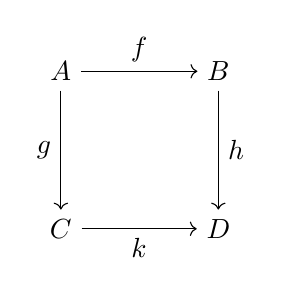
\begin{tikzpicture}
            \node (A) at (0,0) {\(A\)};
            \node (B) at (2,0) {\(B\)};
            \node (C) at (0,-2) {\(C\)};
            \node (D) at (2,-2) {\(D\)};
            \draw[->] (A) -- node[above] {\(f\)} (B);
            \draw[->] (A) -- node[left] {\(g\)} (C);
            \draw[->] (B) -- node[right] {\(h\)} (D);
            \draw[->] (C) -- node[below] {\(k\)} (D);
        \end{tikzpicture}
    \end{center}
    图表交换意味着两点间任意态射合成均相等, 比如 \(h \circ f = k \circ g\).
\end{definition}

\begin{example}
    定义 \(\mathbf{Set}\) 为集合范畴, 其中对象为集合, 对象间态射为映射.
\end{example}

\begin{example}
    定义 \(\mathbf{0}\) 为空范畴, 也即 \(\mathrm{Ob} (\mathbf{0}) = \emptyset\).
\end{example}

\begin{example}
    对偏序集 \(P\), 定义其对应的范畴 \(\mathrm{Cat} (P)\) 如下:

    \begin{enumerate}
        \item 对象是 \(P\) 中的元素.
        \item \(x \leq y\) 时有唯一态射 \(x \to y\).
        \item \(x \nleq y\) 时没有态射.
    \end{enumerate}
\end{example}

\begin{definition}
    对集合 \(S\) 定义离散范畴 \(\mathrm{Disc} (S)\) 如下:

    \begin{enumerate}
        \item 对象是 \(S\) 中的元素.
        \item 仅有单位态射.
    \end{enumerate}
\end{definition}

\begin{definition}
    若有一组映射 \(f : X \to Y\), \(g : Y \to X\) 使得 \(g \circ f = \mathrm{id}_X\), \(f \circ g = \mathrm{id}_Y\), 则称 \(f\) 为 \(g\) 的逆, \(f\) 是同构,
    记作 \(f^{-1} = g\).

    \(X\) 与 \(Y\) 同构记作 \(X \cong Y\), 命全体 \(X\) 与 \(Y\) 间的同构为 \(\mathrm{Isom}_{\mathcal{C}} (X,Y)\).
\end{definition}

\begin{definition}
    定义自同态集 \(\mathrm{End}_{\mathcal{C}} (X) := \mathrm{Hom}_{\mathcal{C}} (X,X)\) 与自同构集
    \(\mathrm{Aut}_{\mathcal{C}} (X) := \mathrm{Isom}_{\mathcal{C}} (X,X)\), 其上有自然的复合运算.
\end{definition}

\begin{definition}
    态射 \(f : X \to Y\) 称为单态射 (monomorphism), 如果对于任意 \(g,h : Z \to X\), 有 \(f \circ g = f \circ h \implies g = h\).

    态射 \(f : X \to Y\) 称为满态射 (epimorphism), 如果对于任意 \(g,h : Y \to Z\), 有 \(g \circ f = h \circ f \implies g = h\).
\end{definition}

\begin{definition}[反范畴]
    定义范畴 \(\mathcal{C}^{\mathrm{op}}\) 如下:

    \begin{enumerate}
        \item \(\mathrm{Ob} (\mathcal{C}^{\mathrm{op}}) = \mathrm{Ob} (\mathcal{C})\).
        \item \(\mathrm{Hom}_{\mathcal{C}^{\mathrm{op}}} (X,Y) = \mathrm{Hom}_{\mathcal{C}} (Y,X)\).
        \item 对于态射 \(f : X \to Y, g : Y \to Z\), 定义 \(g \circ_{\mathrm{op}} f := f \circ g\).
    \end{enumerate}
\end{definition}

\begin{definition}[函子]
    \label {definition:functor}
    一个函子 \(F : \mathcal{C} \to \mathcal{D}\) 包含以下资料:

    \begin{enumerate}
        \item 对象映射 \(F : \mathrm{Ob} (\mathcal{C}) \to \mathrm{Ob} (\mathcal{D})\).
        \item 对于任意对象 \(X,Y \in \mathcal{C}\), 有映射 \(F : \mathrm{Hom}_{\mathcal{C}} (X,Y) \to \mathrm{Hom}_{\mathcal{D}} (F(X),F(Y))\).
        \item 对于任意对象 \(X \in \mathcal{C}\), 映单位态射为单位态射 \(F(\mathrm{id}_X) = \mathrm{id}_{F(X)}\).
        \item 对于任意对象 \(X,Y,Z \in \mathcal{C}\) 保持态射的复合 \(F(g \circ f) = F(g) \circ F(f)\).
    \end{enumerate}
\end{definition}

\begin{definition}[反变函子]
    定义 \(\mathcal{C}\) 出发反变函子为从其反范畴出发的函子.
\end{definition}

\begin{definition}
    一个函子称为忠实 (faithful), 如果对于任意对象 \(X,Y \in \mathcal{C}\), 映射 \(F : \mathrm{Hom}_{\mathcal{C}} (X,Y) \to \mathrm{Hom}_{\mathcal{D}} (F(X),F(Y))\) 是单射.

    一个函子称为全 (full), 如果对于任意对象 \(X,Y \in \mathcal{C}\), 映射 \(F : \mathrm{Hom}_{\mathcal{C}} (X,Y) \to \mathrm{Hom}_{\mathcal{D}} (F(X),F(Y))\) 是满射.

    一个函子称本质满 (essentially surjective), 如果对于任意对象 \(Y \in \mathcal{D}\), 存在对象 \(X \in \mathcal{C}\) 使得 \(F(X) \cong Y\).
\end{definition}

\begin{definition}
    对于函子 \(F : \mathcal{C} \to \mathcal{D}\), \(G : \mathcal{D} \to \mathcal{E}\), 定义函子间的复合 \((G \circ F) (X) := G(F(X))\), \((G \circ F) (f) := G(F(f))\).

    \begin{proof}
        只需注意到 \(G(F(f)) \circ G(F(g)) = G(F(f) \circ F(g)) = G(F(f \circ g))\).
    \end{proof}
\end{definition}

\begin{definition}
    显见函子复合满足结合律, 定义范畴 \(\mathbf{Cat}\) 如下:

    \begin{enumerate}
        \item 对象是 \(\mathrm{Ob} (\mathcal{C}), \mathrm{Mor} (\mathcal{C})\) 是集合的范畴 \(\mathcal{C}\).
        \item \(\mathrm{Hom}_{\mathbf{Cat}} (\mathcal{C},\mathcal{D})\) 是所有函子 \(\mathcal{C} \to \mathcal{D}\).
    \end{enumerate}
\end{definition}

\begin{definition}[自然变换]
    两个函子 \(F,G : \mathcal{C} \to \mathcal{D}\) 之间的自然变换 (natural transformation) \(\eta : F \to G\) 为对所有 \(X \in \mathrm{Ob} (C)\) 择定的态射 \(\eta_X : F(X) \to G(X)\),
    满足对于任意对象 \(X,Y \in \mathcal{C}\) 与 \(f \in \mathrm{Hom}_{\mathcal{C}} (X,Y)\), 有交换图表:
        
    \begin{center}
        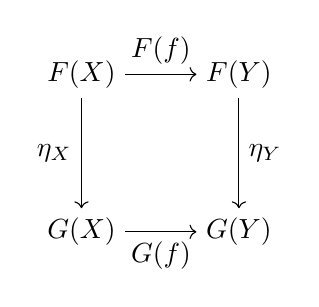
\begin{tikzpicture}
            \node (FX) at (0,0) {\(F(X)\)};
            \node (FY) at (2,0) {\(F(Y)\)};
            \node (GX) at (0,-2) {\(G(X)\)};
            \node (GY) at (2,-2) {\(G(Y)\)};
            \draw[->] (FX) -- node[above] {\(F(f)\)} (FY);
            \draw[->] (FX) -- node[left] {\(\eta_X\)} (GX);
            \draw[->] (FY) -- node[right] {\(\eta_Y\)} (GY);
            \draw[->] (GX) -- node[below] {\(G(f)\)} (GY);
        \end{tikzpicture}
    \end{center}

    记作 \(\eta : F \to G\), 可以画作图表:

    \begin{center}
        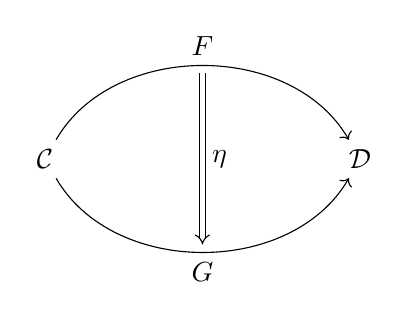
\begin{tikzpicture}
            \node (C) at (-2,0) {\(\mathcal{C}\)};
            \node (D) at (2,0) {\(\mathcal{D}\)};
            \draw[->] (C) to[bend left=60] node[above] (F) {\(F\)} (D);
            \draw[->] (C) to[bend right=60] node[below] (G) {\(G\)} (D);
            \draw[double,-{Implies},double distance = 0.15em] ($(F.south) + (0,- 0.1)$) to node[right] {\(\eta\)} ($(G.north) + (0,0.1)$);
        \end{tikzpicture}
    \end{center}
\end{definition}

\begin{definition}[纵合成]
    给出 \(\eta : F \to G\), \(\theta : G \to H\), 定义纵合成 \(\theta \circ \eta : F \to H\) 为 \({(\theta \circ \eta)}_X := \theta_X \circ \eta_X\), 解作图表:
    
    \[
        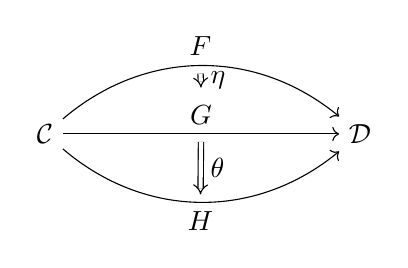
\begin{tikzpicture}
            \node (C) at (-2,0) {\(\mathcal{C}\)};
            \node (D) at (2,0) {\(\mathcal{D}\)};
            \draw[->] (C) to[bend left=40] node[above] (F) {\(F\)} (D);
            \draw[->] (C) to node[above] (G) {\(G\)} (D);
            \draw[->] (C) to[bend right=40] node[below] (H) {\(H\)} (D);
            \draw[double,-{Implies},double distance = 0.15em] ($(F.south) + (0,- 0.1)$) to node[right] {\(\eta\)} ($(G.north) + (0,0.1)$);
            \draw[double,-{Implies},double distance = 0.15em] ($(G.south) + (0,- 0.1)$) to node[right] {\(\theta\)} ($(H.north) + (0,0.1)$);
        \end{tikzpicture} = 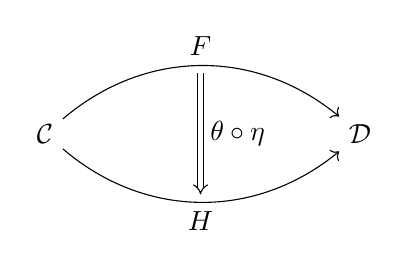
\begin{tikzpicture}
            \node (C) at (-2,0) {\(\mathcal{C}\)};
            \node (D) at (2,0) {\(\mathcal{D}\)};
            \draw[->] (C) to[bend left=40] node[above] (F) {\(F\)} (D);
            \draw[->] (C) to[bend right=40] node[below] (H) {\(H\)} (D);
            \draw[double,-{Implies},double distance = 0.15em] ($(F.south) + (0,- 0.1)$) to node[right] {\(\theta \circ \eta\)} ($(H.north) + (0,0.1)$);
        \end{tikzpicture}
    \]

    \begin{proof}
        只需注意到以下交换图表 (两小方块交换故外框交换):

        \begin{center}
            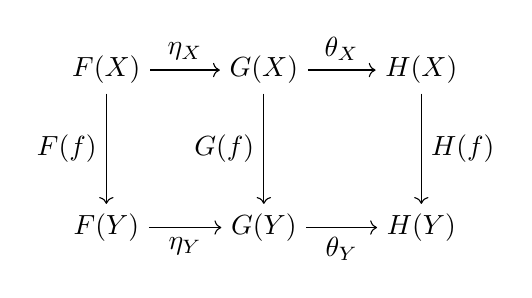
\begin{tikzpicture}
                \node (FX) at (-2,1) {\(F(X)\)};
                \node (FY) at (-2,-1) {\(F(Y)\)};
                \node (GX) at (0,1) {\(G(X)\)};
                \node (GY) at (0,-1) {\(G(Y)\)};
                \node (HX) at (2,1) {\(H(X)\)};
                \node (HY) at (2,-1) {\(H(Y)\)};
                \draw[->] (FX) -- node[left] {\(F(f)\)} (FY);
                \draw[->] (FX) -- node[above] {\(\eta_X\)} (GX);
                \draw[->] (FY) -- node[below] {\(\eta_Y\)} (GY);
                \draw[->] (GX) -- node[left] {\(G(f)\)} (GY);
                \draw[->] (GX) -- node[above] {\(\theta_X\)} (HX);
                \draw[->] (GY) -- node[below] {\(\theta_Y\)} (HY);
                \draw[->] (HX) -- node[right] {\(H(f)\)} (HY);
            \end{tikzpicture}
        \end{center}
    \end{proof}
\end{definition}

\begin{definition}[横合成]
    给出三个范畴 \(\mathcal{C},\mathcal{D},\mathcal{E}\) 以及四个函子 \(F_1,F_2 : \mathcal{C} \to \mathcal{D}\), \(G_1,G_2 : \mathcal{D} \to \mathcal{E}\), 
    给出自然变换 \(\eta : F_1 \to F_2\), \(\theta : G_1 \to G_2\), 定义横合成 \(\theta \ast \eta : G_1 \circ F_1 \to G_2 \circ F_2\) 为 \({(\theta \ast \eta)}_X := \theta_{F_2 (X)} \circ G_1 (\eta_X)\), 解作图表:

    \[
        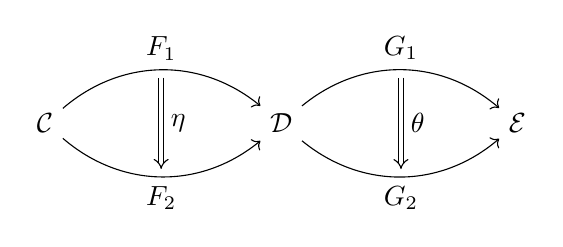
\begin{tikzpicture}
            \node (C) at (-3,0) {\(\mathcal{C}\)};
            \node (D) at (0,0) {\(\mathcal{D}\)};
            \node (E) at (3,0) {\(\mathcal{E}\)};
            \draw[->] (C) to[bend left=40] node[above] (F1) {\(F_1\)} (D);
            \draw[->] (C) to[bend right=40] node[below] (F2) {\(F_2\)} (D);
            \draw[->] (D) to[bend left=40] node[above] (G1) {\(G_1\)} (E);
            \draw[->] (D) to[bend right=40] node[below] (G2) {\(G_2\)} (E);
            \draw[double,-{Implies},double distance = 0.15em] ($(F1.south) + (0,- 0.1)$) to node[right] {\(\eta\)} ($(F2.north) + (0,0.1)$);
            \draw[double,-{Implies},double distance = 0.15em] ($(G1.south) + (0,- 0.1)$) to node[right] {\(\theta\)} ($(G2.north) + (0,0.1)$);
        \end{tikzpicture} = 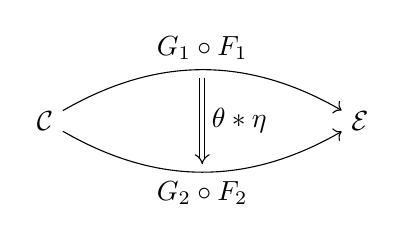
\begin{tikzpicture}
            \node (C) at (-2,0) {\(\mathcal{C}\)};
            \node (E) at (2,0) {\(\mathcal{E}\)};
            \draw[->] (C) to[bend left=30] node[above] (G1F1) {\(G_1 \circ F_1\)} (E);
            \draw[->] (C) to[bend right=30] node[below] (G2F2) {\(G_2 \circ F_2\)} (E);
            \draw[double,-{Implies},double distance = 0.15em] ($(G1F1.south) + (0,- 0.1)$) to node[right] {\(\theta \ast \eta\)} ($(G2F2.north) + (0,0.1)$);
        \end{tikzpicture}
    \]

    \begin{proof}
        需注意到以下交换图表:

        \begin{center}
            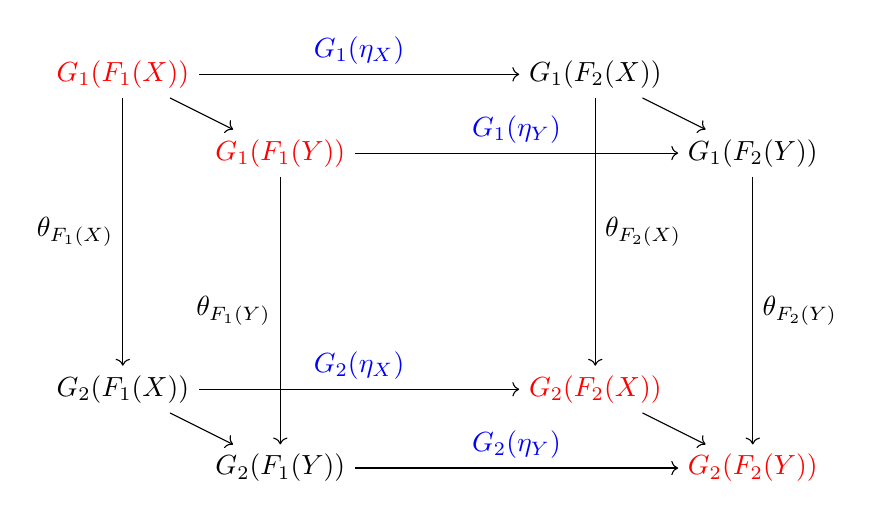
\begin{tikzpicture}
                \node (G1F1X) at (-4,4) {\textcolor{red}{\(G_1 (F_1 (X))\)}};
                \node (G1F1Y) at (-2,3) {\textcolor{red}{\(G_1 (F_1 (Y))\)}};
                \node (G1F2X) at (2,4) {\(G_1 (F_2 (X))\)};
                \node (G1F2Y) at (4,3) {\(G_1 (F_2 (Y))\)};
                \node (G2F1X) at (-4,0) {\(G_2 (F_1 (X))\)};
                \node (G2F1Y) at (-2,-1) {\(G_2 (F_1 (Y))\)};
                \node (G2F2X) at (2,0) {\textcolor{red}{\(G_2 (F_2 (X))\)}};
                \node (G2F2Y) at (4,-1) {\textcolor{red}{\(G_2 (F_2 (Y))\)}};
                \draw[->] (G1F1X) -- (G1F1Y);
                \draw[->] (G1F2X) -- (G1F2Y);
                \draw[->] (G2F1X) -- (G2F1Y);
                \draw[->] (G2F2X) -- (G2F2Y);
                \draw[->] (G1F1X) -- node[above] {\textcolor{blue}{\(G_1 (\eta_X)\)}} (G1F2X);
                \draw[->] (G1F1Y) -- node[above] {\textcolor{blue}{\(G_1 (\eta_Y)\)}} (G1F2Y);
                \draw[->] (G2F1X) -- node[above] {\textcolor{blue}{\(G_2 (\eta_X)\)}} (G2F2X);
                \draw[->] (G2F1Y) -- node[above] {\textcolor{blue}{\(G_2 (\eta_Y)\)}} (G2F2Y);
                \draw[->] (G1F1X) -- node[left] {{\(\theta_{F_1 (X)}\)}} (G2F1X);
                \draw[->] (G1F1Y) -- node[left] {\(\theta_{F_1 (Y)}\)} (G2F1Y);
                \draw[->] (G1F2X) -- node[right] {\(\theta_{F_2 (X)}\)} (G2F2X);
                \draw[->] (G1F2Y) -- node[right] {\(\theta_{F_2 (Y)}\)} (G2F2Y);
            \end{tikzpicture}
        \end{center}

        前后左右四面交换源自 \(\theta\) 为自然变换, 上下两面交换源自 \(\eta\) 为自然变换, 于是\textcolor{red}{红色}标记出的子图亦交换.
    \end{proof}
\end{definition}

特别的, 在标记自然变换时, 我们可以将单独的函子 \(F\) 拉开成为 \(\mathrm{id}_F : F \to F\), 在每个 \(X\) 上为 \(\mathrm{id}_{F(X)}\).

\begin{definition}
    对于范畴 \(\mathcal{C}, \mathcal{D}\), 定义函子范畴 \(\mathbf{Fun} (\mathcal{C},\mathcal{D})\) 如下:

    \begin{enumerate}
        \item 对象是函子 \(\mathcal{C} \to \mathcal{D}\).
        \item 对于函子 \(F,G : \mathcal{C} \to \mathcal{D}\), 定义态射集 \(\mathrm{Hom}_{\mathbf{Fun} (\mathcal{C},\mathcal{D})} (F,G)\) 为所有 \(F \to G\) 的自然变换.
        \item 态射的合成是自然变换的纵合成.
    \end{enumerate}

    \begin{proof}
        只需证明纵合成之结合律, 只需注意到态射结合律:

        \[
            (\theta_X \circ \eta_X) \circ \phi_X = \theta_X \circ (\eta_X \circ \phi_X)
        \]
    \end{proof}
\end{definition}

\begin{lemma}
    函子的纵合成满足结合律.

    \begin{proof}
        给出自然变换 \(\theta, \psi, \phi\) 如下:

        \begin{center}
            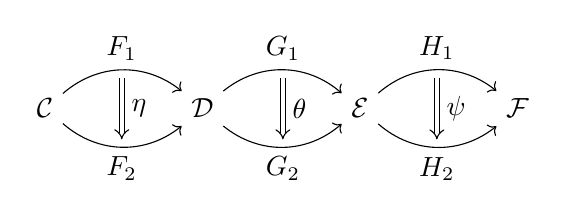
\begin{tikzpicture}
                \node (C) at (-3,0) {\(\mathcal{C}\)};
                \node (D) at (-1,0) {\(\mathcal{D}\)};
                \node (E) at (1,0) {\(\mathcal{E}\)};
                \node (F) at (3,0) {\(\mathcal{F}\)};
                \draw[->] (C) to[bend left=40] node[above] (F1) {\(F_1\)} (D);
                \draw[->] (C) to[bend right=40] node[below] (F2) {\(F_2\)} (D);
                \draw[->] (D) to[bend left=40] node[above] (G1) {\(G_1\)} (E);
                \draw[->] (D) to[bend right=40] node[below] (G2) {\(G_2\)} (E);
                \draw[->] (E) to[bend left=40] node[above] (H1) {\(H_1\)} (F);
                \draw[->] (E) to[bend right=40] node[below] (H2) {\(H_2\)} (F);
                \draw[double,-{Implies},double distance = 0.15em] ($(F1.south) + (0,- 0.1)$) to node[right] {\(\eta\)} ($(F2.north) + (0,0.1)$);
                \draw[double,-{Implies},double distance = 0.15em] ($(G1.south) + (0,- 0.1)$) to node[right] {\(\theta\)} ($(G2.north) + (0,0.1)$);
                \draw[double,-{Implies},double distance = 0.15em] ($(H1.south) + (0,- 0.1)$) to node[right] {\(\psi\)} ($(H2.north) + (0,0.1)$);
            \end{tikzpicture}
        \end{center}

        有交换图表 (交换性源自于施 \(\psi\) 自然性于 \(G_2 \eta_X\)):

        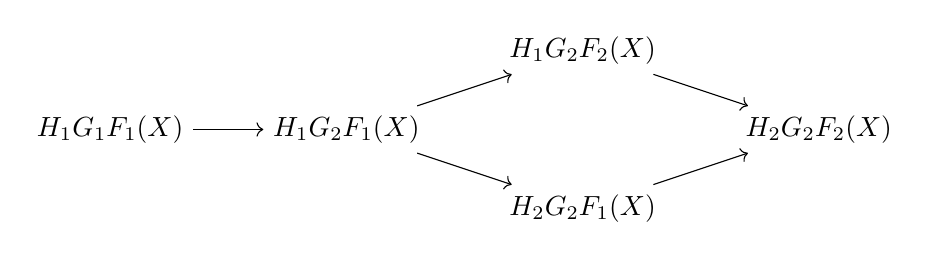
\begin{tikzpicture}
            \node (H1G1F1) at (-4.5,0) {\(H_1 G_1 F_1 (X)\)};
            \node (H1G2F1) at (-1.5,0) {\(H_1 G_2 F_1 (X)\)};
            \node (H1G2F2) at (1.5,1) {\(H_1 G_2 F_2 (X)\)};
            \node (H2G2F2) at (4.5,0) {\(H_2 G_2 F_2 (X)\)};
            \node (H2G2F1) at (1.5,-1) {\(H_2 G_2 F_1 (X)\)};
            \draw[->] (H1G1F1) -- (H1G2F1);
            \draw[->] (H1G2F1) -- (H1G2F2);
            \draw[->] (H1G2F2) -- (H2G2F2);
            \draw[->] (H1G2F1) -- (H2G2F1);
            \draw[->] (H2G2F1) -- (H2G2F2);
        \end{tikzpicture}
    \end{proof}
\end{lemma}

\begin{lemma}
    函子的横纵合成交换, 即亦给出自然变换如下:

    \begin{center}
        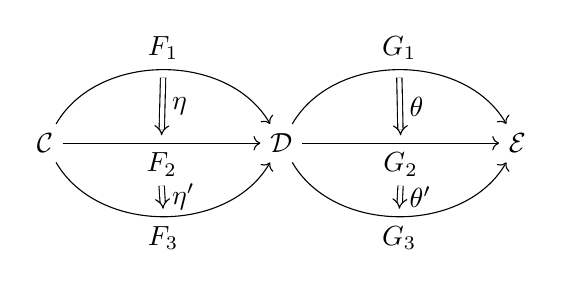
\begin{tikzpicture}
            \node (C) at (-3,0) {\(\mathcal{C}\)};
            \node (D) at (0,0) {\(\mathcal{D}\)};
            \node (E) at (3,0) {\(\mathcal{E}\)};
            \draw[->] (C) to[bend left=60] node[above] (F1) {\(F_1\)} (D);
            \draw[->] (C) to node[below] (F2) {\(F_2\)} (D);
            \draw[->] (C) to[bend right=60] node[below] (F3) {\(F_3\)} (D);
            \draw[->] (D) to[bend left=60] node[above] (G1) {\(G_1\)} (E);
            \draw[->] (D) to node[below] (G2) {\(G_2\)} (E);
            \draw[->] (D) to[bend right=60] node[below] (G3) {\(G_3\)} (E);
            \draw[double,-{Implies},double distance = 0.15em] ($(F1.south) + (0,- 0.1)$) to node[right] {\(\eta\)} ($(F2.north) + (0,0.1)$);
            \draw[double,-{Implies},double distance = 0.15em] ($(F2.south)$) to node[right] {\(\eta^\prime\)} ($(F3.north) + (0,0.1)$);
            \draw[double,-{Implies},double distance = 0.15em] ($(G1.south) + (0,- 0.1)$) to node[right] {\(\theta\)} ($(G2.north) + (0,0.1)$);
            \draw[double,-{Implies},double distance = 0.15em] ($(G2.south)$) to node[right] {\(\theta^\prime\)} ($(G3.north) + (0,0.1)$);
        \end{tikzpicture}
    \end{center}

    则有等式 \((\theta^\prime \ast \eta^\prime) \circ (\theta \ast \eta) = (\theta^\prime \circ \theta) \ast (\eta^\prime \circ \eta)\).

    \begin{proof}
        只需注意到以下交换图表:

        \begin{center}
            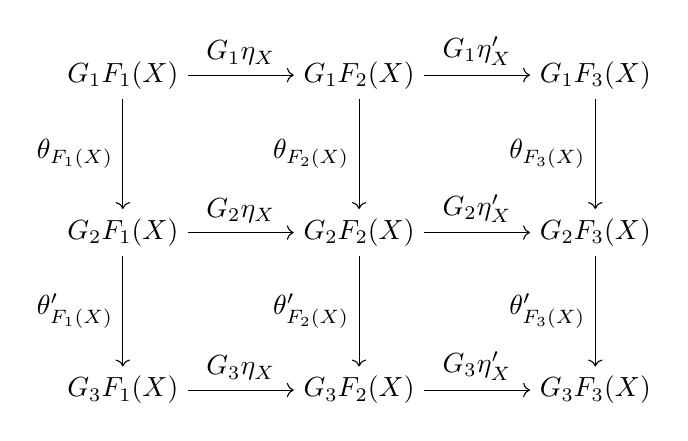
\begin{tikzpicture}
                \node (G1F1X) at (-3,2) {\(G_1 F_1 (X)\)};
                \node (G1F2X) at (0,2) {\(G_1 F_2 (X)\)};
                \node (G1F3X) at (3,2) {\(G_1 F_3 (X)\)};
                \node (G2F1X) at (-3,0) {\(G_2 F_1 (X)\)};
                \node (G2F2X) at (0,0) {\(G_2 F_2 (X)\)};
                \node (G2F3X) at (3,0) {\(G_2 F_3 (X)\)};
                \node (G3F1X) at (-3,-2) {\(G_3 F_1 (X)\)};
                \node (G3F2X) at (0,-2) {\(G_3 F_2 (X)\)};
                \node (G3F3X) at (3,-2) {\(G_3 F_3 (X)\)};
                \draw[->] (G1F1X) to node[above] {\(G_1 \eta_X\)} (G1F2X);
                \draw[->] (G1F2X) to node[above] {\(G_1 \eta^\prime_X\)} (G1F3X);
                \draw[->] (G2F1X) to node[above] {\(G_2 \eta_X\)} (G2F2X);
                \draw[->] (G2F2X) to node[above] {\(G_2 \eta^\prime_X\)} (G2F3X);
                \draw[->] (G3F1X) to node[above] {\(G_3 \eta_X\)} (G3F2X);
                \draw[->] (G3F2X) to node[above] {\(G_3 \eta^\prime_X\)} (G3F3X);
                \draw[->] (G1F1X) to node[left] {\(\theta_{F_1 (X)}\)} (G2F1X);
                \draw[->] (G1F2X) to node[left] {\(\theta_{F_2 (X)}\)} (G2F2X);
                \draw[->] (G1F3X) to node[left] {\(\theta_{F_3 (X)}\)} (G2F3X);
                \draw[->] (G2F1X) to node[left] {\(\theta^\prime_{F_1 (X)}\)} (G3F1X);
                \draw[->] (G2F2X) to node[left] {\(\theta^\prime_{F_2 (X)}\)} (G3F2X);
                \draw[->] (G2F3X) to node[left] {\(\theta^\prime_{F_3 (X)}\)} (G3F3X);
            \end{tikzpicture}
        \end{center}

        每个小正方形交换源于 \(\theta, \theta^\prime\) 为自然变换, 故外框交换.
    \end{proof}
\end{lemma}

\begin{lemma}
    \label {lemma:natural transformation is isomorphism iff each component is isomorphism}
    自然变换 \(\eta : F \to G\) 是同构当且仅当对于任意 \(X \in \mathcal{C}\), \(\eta_X\) 是同构,
    其逆为 \(\eta^{-1} : G \to F\), \(\eta^{-1}_X := {\eta_X}^{-1}\).

    \begin{proof}
        给出其逆业已给出每个 \(\eta_X\) 之逆, 而 \(\eta^{-1}\) 是自然性对应了
        \(\eta\) 自然性的交换图表, 换言之, 以下图表每一小块交换故外框交换.

        \begin{center}
            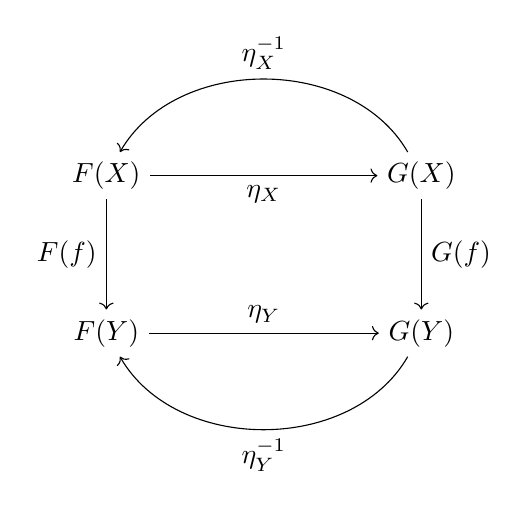
\begin{tikzpicture}
                \node (FX) at (-2,1) {\(F(X)\)};
                \node (FY) at (-2,-1) {\(F(Y)\)};
                \node (GX) at (2,1) {\(G(X)\)};
                \node (GY) at (2,-1) {\(G(Y)\)};
                \draw[->] (FX) to node[left] {\(F(f)\)} (FY);
                \draw[->] (FX) to node[below] {\(\eta_X\)} (GX);
                \draw[->] (FY) to node[above] {\(\eta_Y\)} (GY);
                \draw[->] (GX) to node[right] {\(G(f)\)} (GY);
                \draw[->] (GX) to [bend right=60] node[above] {\(\eta^{-1}_X\)} (FX);
                \draw[->] (GY) to [bend left=60] node[below] {\(\eta^{-1}_Y\)} (FY);
            \end{tikzpicture}
        \end{center}
    \end{proof}
\end{lemma}

\begin{definition}[范畴等价]
    若存在函子 \(F : \mathcal{C} \to \mathcal{D}\), \(G : \mathcal{D} \to \mathcal{C}\) 使得 \(G \circ F \cong \mathrm{id}_{\mathcal{C}}\), \(F \circ G \cong \mathrm{id}_{\mathcal{D}}\), 则称 \(\mathcal{C}\) 与 \(\mathcal{D}\) 等价.

    假定上述定义中 \(\cong\) 为 \(=\), 则称 \(\mathcal{C}\) 与 \(\mathcal{D}\) 同构.
\end{definition}

\begin{definition}[子范畴]
    给定范畴 \(\mathcal{C}^\prime, \mathcal{C}\), 若 \(\mathrm{Ob} (\mathcal{C}^\prime) \subseteq \mathrm{Ob} (\mathcal{C})\), 
    \(\mathrm{Hom}_{\mathcal{C}^\prime} (X,Y) \subseteq \mathrm{Hom}_{\mathcal{C}} (X,Y)\), 且保持复合运算,
    则称 \(\mathcal{C}^\prime\) 是 \(\mathcal{C}\) 的子范畴 (subcategory), 子范畴对应一个自然的嵌入 \(\iota : \mathcal{C}^\prime \to \mathcal{C}\),
    总是忠实, 子范畴亦有全和本质满的性质.
\end{definition}

\begin{definition}[骨架]
    如果范畴 \(\mathcal{C}^\prime\) 是 \(\mathcal{C}\) 的全子范畴, 且对于任意 \(X \in \mathrm{Ob} (\mathcal{C})\),
    都存在唯一 \(X^\prime \in \mathrm{Ob} (\mathcal{C}^\prime)\) 使得 \(X \cong X^\prime\), 则称 \(\mathcal{C}^\prime\) 是 \(\mathcal{C}\) 的骨架 (skeleton).

    自身是骨架的范畴称为骨架范畴 (skeletal category).
\end{definition}

\begin{definition}[小范畴]
    为了避免一些集合论的困难, 我们定义小范畴 (small category) 为态射类是集合的范畴.

    给出一个 Grothendieck 宇宙 \(\mathcal{U}\), 定义 \(\mathcal{U}\)-小范畴为对象类是 \(\mathcal{U}\) 中的集合的范畴.
\end{definition}

\begin{lemma}
    任何小范畴 \(\mathcal{C}\) 有骨架, 且骨架范畴与 \(\mathcal{C}\) 等价.

    \begin{proof}
        注意到 \(\cong\) 显见的是 \(\mathrm{Ob} (\mathcal{C})\) 上的等价关系, 在每个等价类
        上使用 \ref{axiom:NBG Axiom of Choice} 选取代表元 \(X^\prime\), 与等价类中任意一 \(X\) 与 \(X^\prime\) 间同构 \(f_X : X \to X^\prime\),
        选取子范畴 \(\mathcal{C}^\prime\) 如下:

        \begin{enumerate}
            \item 对象集为全体代表元 \(X^\prime\).
            \item 对于任意 \(X^\prime,Y^\prime \in \mathrm{Ob} (\mathcal{C}^\prime)\), \(\mathrm{Hom}_{\mathcal{C}^\prime} (X^\prime,Y^\prime) = \mathrm{Hom}_{\mathcal{C}} (X^\prime,Y^\prime) \).
        \end{enumerate}

        定义 \(\iota^{-1}\) 映 \(X\) 为其代表元 \(X^\prime\), 映 \(f \in \mathrm{Hom}_{\mathcal{C}} (X,Y)\) 为 
        \(f_Y \circ f \circ {f_X}^{-1}\).

        \(\iota^{-1}\) 函子性, \(\iota \circ \iota^{-1} = \mathrm{id}_{\mathcal{C}}\) 是显然的, 而构造 \(\iota^{-1} \circ \iota \cong \mathrm{id}_{\mathcal{C}^\prime}\) 的自然变换为 \(f\) 即可.
    \end{proof}
\end{lemma}

\begin{lemma}
    范畴等价具有传递性.

    \begin{proof}
        给出范畴 \(\mathcal{C},\mathcal{D},\mathcal{E}\), 函子 \(F : \mathcal{C} \to \mathcal{D}\), \(G : \mathcal{D} \to \mathcal{E}\), 
        以及其逆, 给出可逆的自然变换 \(\eta : F \circ F^{-1} \to \mathrm{id}_{\mathcal{D}}\), \(\theta : F^{-1} \circ F \to \mathrm{id}_{\mathcal{C}}\),
        \(\eta^\prime : G \circ G^{-1} \to \mathrm{id}_{\mathcal{E}}\), \(\theta^\prime : G^{-1} \circ G \to \mathrm{id}_{\mathcal{D}}\), 构造自然变换
        \(\eta^\prime \circ (\mathrm{id}_G \ast \eta \ast \mathrm{id}_{G^{-1}}) : G \circ F \circ F^{-1} \circ G^{-1} \to \mathrm{id}_{\mathcal{E}}\) 有逆
        \((\mathrm{id}_G \ast \eta^{-1} \ast \mathrm{id}_{G^{-1}}) \circ {\eta^{\prime}}^{-1}\),  \(\theta\) 侧可同理构造.
    \end{proof}
\end{lemma}

\begin{lemma}
    骨架范畴间的全忠实本质满函子都是同构.

    \begin{proof}
        本质满则在对象集上是双射, 全忠实亦给出每个态射集上的双射.
    \end{proof}
\end{lemma}

\begin{lemma}
    小范畴间函子 \(F\) 是等价当且仅当 \(F\) 全忠实本质满.

    \begin{proof}
        易得骨架范畴间的同构, 考虑等价的传递性即可.
    \end{proof}
\end{lemma}

\subsection{Hom 函子与泛性质}

\begin{definition}
    对于集合 \(I\) 与小范畴 \({(\mathcal{C}_i)}_{i \in I}\), 定义积范畴 \(\prod_{i \in I} \mathcal{C}_i\) 如下:

    \begin{enumerate}
        \item 对象是积 \(\prod_{i \in I} \mathrm{Ob} (\mathcal{C}_i)\) 的元素.
        \item 对于对象 \((X_i)_{i \in I}\), \((Y_i)_{i \in I}\), 定义态射集 \(\mathrm{Hom}_{\prod_{i \in I} \mathcal{C}_i} ((X_i)_{i \in I},(Y_i)_{i \in I})\) 为态射集之积
                \(\prod_{i \in I} \mathrm{Hom}_{\mathcal{C}_i} (X_i,Y_i)\).
        \item 态射的合成是逐点的, 也即 \({(f_i)}_{i \in I} \circ {(g_i)}_{i \in I} = {(f_i \circ g_i)}_{i \in I}\).
    \end{enumerate}

    定义余积范畴 \(\coprod_{i \in I} \mathcal{C}_i\) 如下:

    \begin{enumerate}
        \item 对象是无交并 \(\coprod_{i \in I} \mathrm{Ob} (\mathcal{C}_i)\) 的元素.
        \item 对象 \(X,Y\) 间有态射当且仅当其对应同一个 \(\mathcal{C}_i\), 态射集继承自 \(\mathcal{C}_i\).
    \end{enumerate}

    定义自明的投影函子 \(\mathbf{Pr}_j : \prod_{i \in I} \mathcal{C}_i \to \mathcal{C}_j\) 与包含函子 \(\mathbf{In}_j : \mathcal{C}_j \to \coprod_{i \in I} \mathcal{C}_i\).
\end{definition}

\begin{definition}
    多元函子即为从积范畴出发的函子.
\end{definition}

\begin{definition}[Hom 函子]
    对于任意范畴 \(\mathcal{C}\), 有函子 \(\mathrm{Hom}_{\mathcal{C}} (-,-) : \mathcal{C}^{\mathrm{op}} \times \mathcal{C} \to \mathbf{Set}\), 映 \((X,Y)\) 为态射集 \(\mathrm{Hom}_{\mathcal{C}} (X,Y)\), 
    映 \(\mathcal{C}^{\mathrm{op}} \times \mathcal{C}\) 中态射 \((f,g)\) 为映射 \(\phi \mapsto g \circ \phi \circ f\).

    称 \(\phi\) 对 \(f\) 做拉回 (pullback), 对 \(g\) 做推出 (pushforward).
\end{definition}

\begin{lemma}
    存在自然同构 \({(\mathbf{Fun} (\mathcal{C}_1 ,\mathcal{C}_2))}^\mathrm{op} \cong \mathbf{Fun} ({\mathcal{C}_1}^\mathrm{op}, {\mathcal{C}_2}^\mathrm{op})\).
\end{lemma}

\begin{lemma}
    有恒等式 \(\mathbf{Fun} (\mathrm{Disc} (I), \mathcal{C}) \cong \prod_{i \in I} \mathcal{C}\).
\end{lemma}

\begin{definition}[中心]
    一个范畴的中心定义为 \(\mathrm{Z} (\mathcal{C}) := \mathrm{End} (\mathrm{id}_{\mathcal{C}})\).

    对范畴等价 \(F : \mathcal{C} \to \mathcal{D}\), 诱导出中心的同构 \(\mathrm{Z} (\mathcal{C}) \cong \mathrm{Z} (\mathcal{D})\).
\end{definition}

\begin{definition}
    假设范畴 \(\mathcal{C}\) 中对象 \(X\) 满足任意 \(Y \in \mathrm{Ob} (\mathcal{C})\), \(\mathrm{Hom}_{\mathcal{C}} (X,Y)\) 是单点集, 则称 \(X\) 是始对象 (initial object).
    对称的 \(\mathrm{Hom}_{\mathcal{C}} (Y,X)\) 是单点集的对象称为终对象 (terminal object).既是始对象又是终对象的对象称为零对象 (zero object).
\end{definition}

\begin{example}
    在 \(\mathbf{Set}\) 中, 空集是始对象, 任意单点集是终对象.
\end{example}

\begin{definition}
    始对象间有唯一的同构, 终对象亦然.

    \begin{proof}
        给出始对象 \(X,Y\), 存在唯一的 \(f : X \to Y\), \(g : Y \to X\),
        同样存在唯一的 \(\mathrm{id}_X : X \to X\), \(\mathrm{id}_Y : Y \to Y\), 于是 \(f \circ g = \mathrm{id}_Y\), \(g \circ f = \mathrm{id}_X\).

        终对象只需注意到任意 \(\mathcal{C}\) 的终对象都是 \(\mathcal{C}^{\mathrm{op}}\) 的始对象.
    \end{proof}
\end{definition}

\begin{definition}
    泛性质 (universal property) 是一种在某个范畴下是始对象或终对象的性质, 其有自然的唯一性.
\end{definition}

\begin{definition}[图范畴]
    给出一个图表样式, 定义该图的范畴如下:

    \begin{enumerate}
        \item 对象是所有使得图表交换的一种填涂方式.
        \item 态射是相同位置的对象逐点的态射, 满足生成的柱状图表交换.
    \end{enumerate}
\end{definition}

\begin{example}[态射范畴]
    称下图的图范畴为 \(\mathcal{C}\) 的态射范畴:

    \begin{center}
        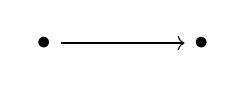
\begin{tikzpicture}
            \node (P1) at (-1,0) {\(\bullet\)};
            \node (P2) at (1,0) {\(\bullet\)};
            \draw[->] (P1) to (P2);
        \end{tikzpicture}
    \end{center}

    即对象是 \(\mathcal{C}\) 中两个对象 \(A,B\) 和一个态射 \(f : A \to B\), 由于确定 \(f\) 亦确定了 \(A,B\),
    也可将对象解作 \(\mathcal{C}\) 中的映射, \(f_1,f_2\) 间的态射是满足以下图表交换的 \((\phi_A, \phi_B)\):

    \begin{center}
        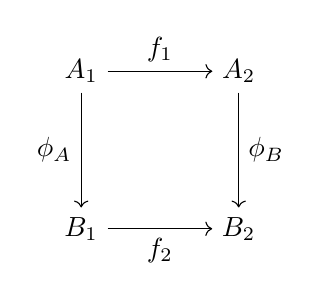
\begin{tikzpicture}
            \node (A1) at (-1,1) {\(A_1\)};
            \node (A2) at (1,1) {\(A_2\)};
            \node (B1) at (-1,-1) {\(B_1\)};
            \node (B2) at (1,-1) {\(B_2\)};
            \draw[->] (A1) to node[above] {\(f_1\)} (A2);
            \draw[->] (B1) to node[below] {\(f_2\)} (B2);
            \draw[->] (A1) to node[left] {\(\phi_A\)} (B1);
            \draw[->] (A2) to node[right] {\(\phi_B\)} (B2);
        \end{tikzpicture}
    \end{center}
\end{example}

\begin{example}[逗号范畴]
    给出函子 \(S : \mathcal{A} \to \mathcal{C}\), \(T : \mathcal{B} \to \mathcal{C}\), 定义逗号范畴 \((S / T)\) 为下图的图范畴:

    \begin{center}
        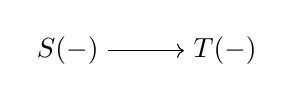
\begin{tikzpicture}
            \node (S) at (-1,0) {\(S (-)\)};
            \node (T) at (1,0) {\(T (-)\)};
            \draw[->] (S) to (T);
        \end{tikzpicture}
    \end{center}

    解作对象是 \(\mathcal{A}\) 中的对象 \(A\), \(\mathcal{B}\) 中的对象 \(B\), 以及 \(\mathcal{C}\) 中的态射 \(f : S(A) \to T(B)\) 组成的 \((A,B,f)\),
    一个 \((A,B,f)\) 到 \((A^\prime,B^\prime,f^\prime)\) 的态射是一对态射 \(g : A \to A^\prime\) 与 \(h : B \to B^\prime\) 使得下图交换:

    \begin{center}
        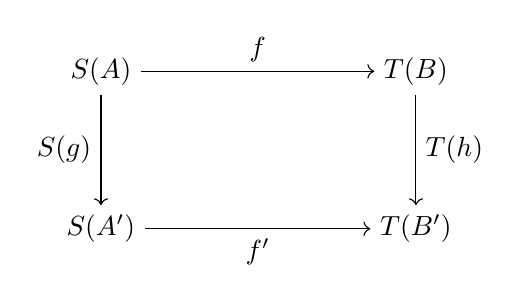
\begin{tikzpicture}
            \node (SA) at (-2,1) {\(S(A)\)};
            \node (TB) at (2,1) {\(T(B)\)};
            \node (SAP) at (-2,-1) {\(S(A^\prime)\)};
            \node (TBP) at (2,-1) {\(T(B^\prime)\)};
            \draw[->] (SA) to node[above] {\(f\)} (TB);
            \draw[->] (SAP) to node[below] {\(f^\prime\)} (TBP);
            \draw[->] (SA) to node[left] {\(S(g)\)} (SAP);
            \draw[->] (TB) to node[right] {\(T(h)\)} (TBP);
        \end{tikzpicture}
    \end{center}
\end{example}

\begin{definition}[子对象, 商对象]
    对 \(X \in \mathrm{Ob} (\mathcal{C})\), 定义 \(X\) 的子对象为单态射 \(i : Y \to X\),
    定义商对象为满态射 \(p : X \to Z\), 在子对象和商对象上定义序:

    定义子对象与商对象的范畴:

    \begin{enumerate}
        \item 对象是 \(X\) 的子对象.
        \item \(i_1 : Y_1 \to X\) 与 \(i_2 : Y_2 \to X\) 的态射是 \(f : Y_1 \to Y_2\) 使得 \(i_1 = i_2 \circ f\).
    \end{enumerate}

    \begin{enumerate}
        \item 对象是 \(X\) 的商对象.
        \item \(p_1 : X \to Z_1\) 与 \(p_2 : X \to Z_2\) 的态射是 \(f : Z_1 \to Z_2\) 使得 \(p_1 = f \circ p_2\).
    \end{enumerate}

    定义子对象与商对象的偏序: \(i_1 \le i_2\) 当且仅当有子对象范畴中的态射 \(f : Y_1 \to Y_2\),
    \(p_1 \le p_2\) 当且仅当有商对象范畴中的态射 \(f : Z_1 \to Z_2\).
\end{definition}

\begin{lemma}
    如果子对象 \(i_1 \le i_2\) 且 \(i_2 \le i_1\), 则子对象 \(i_1\) 与 \(i_2\) 同构, 商对象亦然.

    \begin{proof}
        注意到两个子对象间存在态射则唯一, 于是两个方向均合成为恒等态射.

        商对象无非是 \(\mathcal{C}^{\mathrm{op}}\) 中的子对象.
    \end{proof}
\end{lemma}

\subsection{米田引理}

\begin{definition}[预层]
    给出小范畴 \(\mathcal{C}\), 定义范畴 \(\mathcal{C}^{\vee} : \mathbf{Fun} (\mathcal{C}^{\mathrm{op}}, \mathbf{Set}^{\mathrm{op}})\) 与
    \(\mathcal{C}^{\wedge} : \mathbf{Fun} (\mathcal{C}^{\mathrm{op}}, \mathbf{Set})\), 称 \(\mathcal{C}^{\wedge}\) 为预层 (presheaf) 范畴.
\end{definition}

\begin{definition}
    我们可以自然的将 \(\mathcal{C}\) 嵌入 \(\mathcal{C}^{\wedge}\) 如下:
    \[
        h_{\mathcal{C}} : S \mapsto \mathrm{Hom}_{\mathcal{C}} (-,S)
    \]
    定义自然的求值函子 \(\mathrm{ev}^{\wedge} : \mathcal{C}^{\mathrm{op}} \times \mathcal{C}^{\wedge} \to \mathbf{Set}\) 如下:
    \[
        \mathrm{ev}^{\wedge} (X,S) := S(X)
    \]
    对偶的, 定义 \(k_\mathcal{C} : \mathcal{C} \to \mathcal{C}^{\vee}, \mathrm{ev}^{\vee} : {(\mathcal{C}^{\vee})}^{\mathrm{op}} \times \mathcal{C} \to \mathbf{Set}\) 如下:
    \[
        k_\mathcal{C} (S) := \mathrm{Hom}_{\mathcal{C}} (S,-), \mathrm{ev}^{\vee} (S,X) := S(X)
    \]
\end{definition}

下述引理称米田引理 (Yoneda lemma), 是范畴论中非常重要的引理.

\begin{lemma}[Yoneda]
    \setlabel {米田引理}
    \label {lemma:Yoneda lemma}
    对于任意 \(\mathcal{C}\) 上的预层 \(A \in \mathrm{Ob} (\mathcal{C}^{\wedge})\), 与对象 \(S \in \mathcal{C}\), 
    存在 \(\mathrm{Hom}_{\mathcal{C}^{\wedge}} (h_{\mathcal{C}} (S), A) \cong A(S)\) 的自然双射:
    \[
        (\phi : h_{\mathcal{C}} (S) \to A) \mapsto \phi_S (\mathrm{id}_S)
    \]
    此双射给出 \(\mathrm{Hom}_{\mathcal{C}^{\wedge}} (h_{\mathcal{C}} (-), -)\) 与 \(\mathrm{ev}^{\wedge}\) 的同构.

    \begin{proof}
        证明的技巧在于向层的嵌入将映射转为拉回和推出, 所以对于所有 \(a \in A(S)\), 可以限制出 \(\phi_a : h_{\mathcal{C}} (S) \to A\) 为 \(f \in \mathrm{Hom}_{\mathcal{C}} (X,S)\) 有:
        \[
            \phi_a (f) = \phi_a (\mathrm{id}_S \circ f) = \phi_a (((h_{\mathcal{C}} (S)) (f)) (\mathrm{id}_S)) = A(f) \phi_a (\mathrm{id}_S) = A(f) (a)
        \]
        \begin{center}
            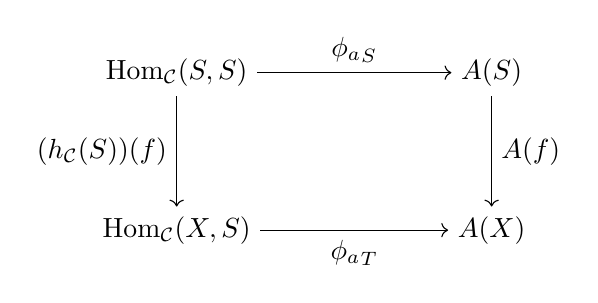
\begin{tikzpicture}
                \node (HSS) at (-2,1) {\(\mathrm{Hom}_{\mathcal{C}} (S,S)\)};
                \node (HXS) at (-2,-1) {\(\mathrm{Hom}_{\mathcal{C}} (X,S)\)};
                \node (AS) at (2,1) {\(A(S)\)};
                \node (AX) at (2,-1) {\(A(X)\)};
                \draw[->] (HSS) to node[left] {\((h_{\mathcal{C}} (S)) (f)\)} (HXS);
                \draw[->] (AS) to node[right] {\(A(f)\)} (AX);
                \draw[->] (HSS) to node[above] {\({\phi_a}_S\)} (AS);
                \draw[->] (HXS) to node[below] {\({\phi_a}_T\)} (AX);
            \end{tikzpicture}
        \end{center}

        自然性展开符号即可, 同构基于 \ref{lemma:natural transformation is isomorphism iff each component is isomorphism}.
    \end{proof}
\end{lemma}

\begin{lemma}
    上述 \(h_\mathcal{C}\) 是全忠实函子, 给出了自然的嵌入 \(\mathcal{C} \to \mathcal{C}^{\wedge}\).

    \begin{proof}
        全忠实性考虑取 \(A\) 为 \(h_\mathcal{C}(T)\), \ref{lemma:Yoneda lemma} 即给出 \(\mathrm{Hom}_{\mathcal{C}^{\wedge}} (h_{\mathcal{C}} (S), h_{\mathcal{C}} (T))\), \(\mathrm{Hom}_{\mathcal{C}} (S,T)\)
        间双射.
    \end{proof}
\end{lemma}

\begin{corollary}
    对称的, \(k_\mathcal{C}\) 全忠实, 且有自然的函子同构 \(\mathrm{Hom}_{\mathcal{C}^{\vee}} (k_{\mathcal{C}} (-), -) \to \mathrm{ev}^{\vee}\).

    \begin{proof}
        只需注意到恒等式 \({(\mathcal{C}^{\vee})}^\mathrm{op} = {(\mathcal{C}^{\mathrm{op}})}^{\wedge}\).
    \end{proof}
\end{corollary}

\begin{definition}[可表]
    称预层 \(A\) 可表 (representable) 当且仅当存在对象 \(S \in \mathcal{C}\) 并给出 \(A \cong h_{\mathcal{C}} (S)\) 的同构 \(\phi : h_{\mathcal{C}} (S) \to A\),
    并称 \((S,\phi)\) 是 \(A\) 的代表元, 对 \(B \in \mathbf{Fun} (\mathcal{C},\mathbf{Set})\) 亦然.
\end{definition}

\begin{lemma}
    代表元若存在则在同构意义下唯一.

    \begin{proof}
        利用米田嵌入的全忠实性.
    \end{proof}
\end{lemma}

\subsection{伴随对}

\begin{definition}[伴随]
    给出函子 \(F : \mathcal{C} \to \mathcal{D}\), \(G : \mathcal{D} \to \mathcal{C}\), 
    与自然变换 \(\eta : \mathrm{id}_{\mathcal{C}} \to G \circ F\), \(\varepsilon : F \circ G \to \mathrm{id}_{\mathcal{D}}\),
    使得以下两图表合成为恒等自然变换:

    \begin{center}
        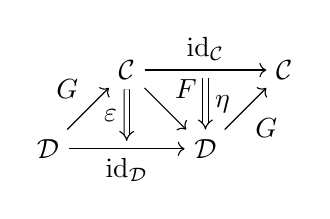
\begin{tikzpicture}
            \node (C1) at (-0.5,0.5) {\(\mathcal{C}\)};
            \node (C2) at (1.5,0.5) {\(\mathcal{C}\)};
            \node (D1) at (-1.5,-0.5) {\(\mathcal{D}\)};
            \node (D2) at (0.5,-0.5) {\(\mathcal{D}\)};
            \draw[->] (C1) to node[above] (idc) {\(\mathrm{id}_{\mathcal{C}}\)} (C2);
            \draw[->] (D1) to node[below] (idd) {\(\mathrm{id}_{\mathcal{D}}\)} (D2);
            \draw[->] (D1) to node[above left] {\(G\)} (C1);
            \draw[->] (D2) to node[below right] {\(G\)} (C2);
            \draw[->] (C1) to node[above right] {\(F\)} (D2);
            \draw[-{Implies},double,double distance = 0.15em] (C1) to node[left] {\(\varepsilon\)} ($(idd.north) + (0,0.1)$);
            \draw[-{Implies},double,double distance = 0.15em] ($(idc.south) + (0,-0.1)$) to node[right] {\(\eta\)} (D2);
        \end{tikzpicture} 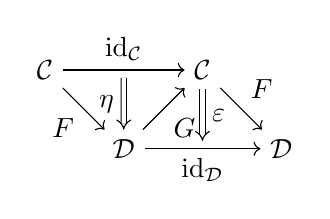
\begin{tikzpicture}
            \node (C1) at (-1.5,0.5) {\(\mathcal{C}\)};
            \node (C2) at (0.5,0.5) {\(\mathcal{C}\)};
            \node (D1) at (-0.5,-0.5) {\(\mathcal{D}\)};
            \node (D2) at (1.5,-0.5) {\(\mathcal{D}\)};
            \draw[->] (C1) to node[above] (idc) {\(\mathrm{id}_{\mathcal{C}}\)} (C2);
            \draw[->] (D1) to node[below] (idd) {\(\mathrm{id}_{\mathcal{D}}\)} (D2);
            \draw[->] (C1) to node[below left] {\(F\)} (D1);
            \draw[->] (C2) to node[above right] {\(F\)} (D2);
            \draw[->] (D1) to node[below right] {\(G\)} (C2);
            \draw[-{Implies},double,double distance = 0.15em] (C2) to node[right] {\(\varepsilon\)} ($(idd.north) + (0,0.1)$);
            \draw[-{Implies},double,double distance = 0.15em] ($(idc.south) + (0,-0.1)$) to node[left] {\(\eta\)} (D1);
        \end{tikzpicture}
    \end{center}

    写成合成为:

    \[
        (\mathrm{id}_{G} \ast \varepsilon) \circ (\eta \ast \mathrm{id}_{G}) = \mathrm{id}_{G}, (\varepsilon \ast \mathrm{id}_{F}) \circ (\mathrm{id}_{F} \ast \eta) = \mathrm{id}_{F}
    \]

    称 \(F\) 为 \(G\) 的左伴随 (left adjoint), \(G\) 为 \(F\) 的右伴随 (right adjoint), 记为 \(F \dashv G\).
\end{definition}

\begin{lemma}
    \(F\) 是 \(G\) 左伴随当且仅当有 \(\mathcal{C}^{\mathrm{op}} \times \mathcal{D} \to \mathbf{Set}\) 中函子
    \(\mathrm{Hom}_{\mathcal{D}} (F (-), -)\) 与 \(\mathrm{Hom}_{\mathcal{C}} (-, G (-))\) 同构.

    \begin{proof}
        我们的任务是找到这样一个一一对应, 这里的技术在于把映射变成拉回推出.

        假定我们给出伴随函子 \(F,G\) 和 \(f \in \mathrm{Hom}_{\mathcal{D}} (F (X), Y)\), 构造
        \(\varphi(f) : X \to G (Y)\) 为 \(G (f) \circ \eta_X\); 对 \(g \in \mathrm{Hom}_{\mathcal{C}} (X, G(Y))\) 构造
        \(\varphi^{-1} (g) : F(X) \to Y\) 为 \(\varepsilon_Y \circ F (g)\).

        而 \(\varphi^{-1} \varphi (f) = \varepsilon_{Y} \circ F (G (f) \circ \eta_X) = (\varepsilon_Y \circ FG f) \circ \eta_X = f \circ \varepsilon_{F(X)} \circ F (\eta_X) = f\),
        \(\varphi \varphi^{-1} (g) = G(\varepsilon_Y \circ F(g)) \circ \eta_X = G (\varepsilon_Y) \circ (GF (g) \circ \eta_{X}) = G (\varepsilon_Y) \circ \eta_{G(Y)} \circ g = g\).

        接下来验证 \(\varphi\) 自然性, \(\varphi(a \circ f \circ F(b)) = G(a) \circ G(f) \circ GF (b) \circ \eta_{X^\prime} = G(a) \circ G(f) \circ \eta_X \circ b\),
        \(\varphi^{-1} (G(a) \circ g \circ b) = \varepsilon_{Y^\prime} \circ FG(a) \circ F(g) \circ F(b) = a \circ \varepsilon_Y \circ F(g) \circ F(b)\).

        反之, 给出 \(\varphi\) 与 \(\varphi^{-1}\), 定义 \(\eta_X := \varphi (\mathrm{id}_{F(X)})\), \(\varepsilon_Y := \varphi^{-1} (\mathrm{id}_{G(Y)})\),
        自然性继承自 \(\varphi\) 与 \(\varphi^{-1}\) 的自然性.

        需验证上述自然变换合成等式 \(G \varepsilon_Y \circ \eta_{G(Y)} = \varphi \varphi^{-1} (\mathrm{id}_{G(Y)} \circ \mathrm{id}_{FGY}) = \mathrm{id}_{G(Y)}\),
        \(\varepsilon_{F(X)} \circ F \eta_X = \varphi^{-1} \varphi (\mathrm{id}_{F(X)} \circ \mathrm{id}_{F \eta_X}) = \mathrm{id}_{F(X)}\).
    \end{proof}
\end{lemma}

上述引理给出了伴随对在 \(\mathrm{Hom}\) 集上的体现, 于是我们可以考虑伴随与可表的关系.

\begin{lemma}
    函子 \(F : \mathcal{C} \to \mathcal{D}\) 有右伴随当且仅当 \(\mathrm{Hom}_{\mathcal{D}} (F (-), Y)\) 对每个 \(Y\) 皆可表.

    \begin{proof}
        我们利用可表函子显式的逐点表示出 \(G\).

        对任意 \(Y\), 假定上述函子被 \((S_Y, \phi_Y)\) 表, 则构造出函子 \(G\) 使得 \(G(Y) = S_Y\),
        对于映射 \(f : Y \to Y^\prime\), 令 \(G(f) : S_Y \to S_{Y^\prime}\) 为与 \({\phi_{Y^\prime}}^{-1} \circ h_{\mathcal{C}} (f) \circ \phi_Y \in \mathrm{Mor} (\mathcal{C}^{\wedge})\)
        对应的唯一映射, 则函子性自然归结于 \(h_\mathcal{C}\) 的函子性.

        注意到 \({(\phi_Y)}_X\) 自然给出了 \(\mathrm{Hom}_{\mathcal{D}} (F (X), Y) \to \mathrm{Hom}_{\mathcal{C}} (X, G(Y))\),
        而用 \(\phi\) 在 \(X\) 处自然性源于 \(\phi_Y\) 的自然性, 在 \(Y\) 处自然性源于 \(G(f)\) 定义确保了在 \(\mathcal{C}^{\wedge}\) 中的自然性, 亦 \(\mathcal{C}\) 中的自然性.
    \end{proof}
\end{lemma}

\begin{corollary}
    同理, \(G\) 有左伴随当且仅当 \(\mathrm{Hom}_{\mathcal{C}} (X, G (-))\) 对每个 \(X\) 皆可表.
\end{corollary}

\begin{lemma}
    一个函子的左伴随若存在则在同构意义下唯一, 右伴随亦然.

    \begin{proof}
        运用上题的想法, 既已给出了 \(\mathcal{C}^{\wedge}\) 中的同构, 则亦是 \(\mathcal{C}\) 中的同构,
        该同构自然性亦通过 \(\mathcal{C}^{\wedge}\) 中保存.
    \end{proof}
\end{lemma}

\begin{lemma}
    \label {lemma:adjoint functor's composition is adjoint}
    给出范畴 \(\mathcal{C}_1, \mathcal{C}_2, \mathcal{C}_3\), 与函子 \(F : \mathcal{C}_1 \to \mathcal{C}_2\), \(G : \mathcal{C}_2 \to \mathcal{C}_1\),
    \(F^\prime : \mathcal{C}_2 \to \mathcal{C}_3\), \(G^\prime : \mathcal{C}_3 \to \mathcal{C}_2\), 使得 \(F \dashv G\), \(F^\prime \dashv G^\prime\),
    则 \(F^\prime \circ F \dashv G \circ G^\prime\).

    \begin{center}
        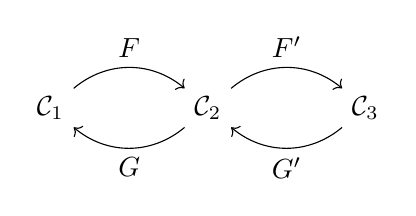
\begin{tikzpicture}
            \node (C1) at (-2,0) {\(\mathcal{C}_1\)};
            \node (C2) at (0,0) {\(\mathcal{C}_2\)};
            \node (C3) at (2,0) {\(\mathcal{C}_3\)};
            \draw[->] (C1) to [bend left = 40] node[above] {\(F\)} (C2);
            \draw[->] (C2) to [bend left = 40] node[above] {\(F^\prime\)} (C3);
            \draw[->] (C2) to [bend left = 40] node[below] {\(G\)} (C1);
            \draw[->] (C3) to [bend left = 40] node[below] {\(G^\prime\)} (C2);
        \end{tikzpicture}
    \end{center}

    \begin{proof}
        给出伴随对应的自然变换 \(\eta, \eta^\prime, \varepsilon, \varepsilon^\prime\),
        定义 \(\xi := (\mathrm{id}_G \ast \eta^\prime \mathrm{id}_{F}) \circ \eta\),
        \(\zeta := \varepsilon^\prime \ast (\varepsilon \ast \mathrm{id}_{G^\prime}) \circ \mathrm{id}_F\),

        \(\xi, \zeta\) 给出 \(F^\prime \circ F \dashv G \circ G^\prime\), 观察以下图表:

        \begin{center}
            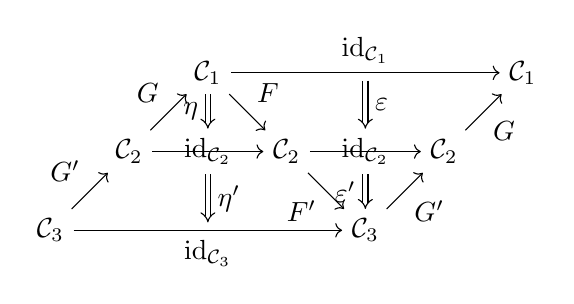
\begin{tikzpicture}
                \node (C11) at (-1,1) {\(\mathcal{C}_1\)};
                \node (C12) at (3,1) {\(\mathcal{C}_1\)};
                \node (C21) at (-2,0) {\(\mathcal{C}_2\)};
                \node (C22) at (0,0) {\(\mathcal{C}_2\)};
                \node (C23) at (2,0) {\(\mathcal{C}_2\)};
                \node (C31) at (-3,-1) {\(\mathcal{C}_3\)};
                \node (C32) at (1,-1) {\(\mathcal{C}_3\)};
                \draw[->] (C11) to node[above] (idc1) {\(\mathrm{id}_{\mathcal{C}_1}\)} (C12);
                \draw[->] (C21) to node (idc21) {\(\mathrm{id}_{\mathcal{C}_2}\)} (C22);
                \draw[->] (C22) to node (idc22) {\(\mathrm{id}_{\mathcal{C}_2}\)} (C23);
                \draw[->] (C31) to node[below] (idc3) {\(\mathrm{id}_{\mathcal{C}_3}\)} (C32);
                \draw[->] (C31) to node[above left] {\(G^\prime\)} (C21);
                \draw[->] (C21) to node[above left] {\(G\)} (C11);
                \draw[->] (C11) to node[above right] {\(F\)} (C22);
                \draw[->] (C22) to node[below left] {\(F^\prime\)} (C32);
                \draw[->] (C32) to node[below right] {\(G^\prime\)} (C23);
                \draw[->] (C23) to node[below right] {\(G\)} (C12);
                \draw[-{Implies},double,double distance = 0.15em] (C11) to node[left] {\(\eta\)} (idc21);
                \draw[-{Implies},double,double distance = 0.15em] (idc21) to node[right] {\(\eta^\prime\)} ($(idc3.north) + (0,0.1)$);
                \draw[-{Implies},double,double distance = 0.15em] (idc22) to node[left] {\(\varepsilon^\prime\)} (C32);
                \draw[-{Implies},double,double distance = 0.15em] ($(idc1.south) + (0,-0.1)$) to node[right] {\(\varepsilon\)} (idc22);
            \end{tikzpicture}
        \end{center}

        此图表合成 \(\mathrm{id}_{G \circ G^\prime}\) 只需注意到上下两个平行四边形均合成单位自然变换, 而左右两个大三角形分别代表 \(\xi, \zeta\),
        另一个图表同理合成 \(\mathrm{id}_{F^\prime \circ F}\).
    \end{proof}
\end{lemma}

\begin{definition}
    我们定义严格的 \(2\) - 范畴为满足如下条件的范畴:

    \begin{enumerate}
        \item 一个范畴 \(\mathcal{C}\).
        \item 任取 \(X,Y \in \mathrm{Ob} (\mathcal{C})\), 有范畴 \(\mathcal{D}\) 使得 \(\mathrm{Mor} (\mathcal{D}) = \mathrm{Hom}_\mathcal{C} (X,Y)\).
        \item 有横合成, 给出 \(f, f^\prime \in \mathrm{Hom}_\mathcal{C} (X,Y)\), \(g, g^\prime \in \mathrm{Hom}_\mathcal{C} (Y,Z)\), 与
                \(2\) - 态射 \(\phi : f \to f^\prime\), \(\psi : g \to g^\prime\), 存在态射 \(\phi \ast \psi : g \circ f \to g^\prime \circ f^\prime\).
        \item 横合成结合, 且与纵合成交换.
        \item 两个单位横合成仍是单位.
    \end{enumerate}
\end{definition}

记原范畴的元素为 \(\mathrm{Mor}_0\), 原范畴的态射为 \(\mathrm{Mor}_1\), 称 \(1\) - 态射, \(2\) - 态射记为 \(\mathrm{Mor}_2\).

\begin{example}
    \(\mathbf{Cat}\) 是严格的 \(2\) - 范畴, 对象是全体小范畴, 态射是范畴间的函子, \(2\) - 态射是自然变换.
\end{example}

我们可以绘制 \(2\) - 范畴对应的图表, 用 \(\Rightarrow\) 表示 \(2\) - 态射, 依旧用 \(\mathrm{Hom}\) 表示两点间态射对应的范畴.

\begin{definition}[Kan 延拓]
    在严格 \(2\) - 范畴 \(\Theta\) 中给出对象 \(\mathcal{C},\mathcal{D},\mathcal{E} \in \mathrm{Mor}_0 (\Theta)\),
    给出 \(1\) - 态射 \(F : \mathcal{C} \to \mathcal{E}, K : \mathcal{C} \to \mathcal{D}\).

    定义左 Kan 延拓 \(\mathrm{Lan}_K F : \mathcal{D} \to \mathcal{E}\) 与其对应的 \(2\) - 态射 \(\eta : F \to \mathrm{Lan}_K F \circ K\),
    满足任给 \(G : \mathcal{D} \to \mathcal{E}\) 与 \(2\) - 态射 \(\phi : F \to G \circ K\), 存在唯一的 \(2\) - 态射 \(\phi^\prime : \mathrm{Lan}_K F \to G\), 满足以下等式:

    \[
        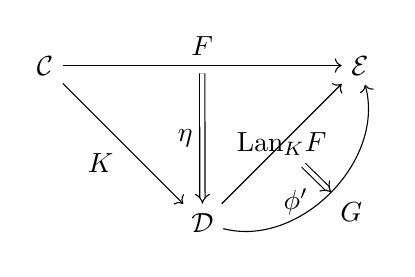
\begin{tikzpicture}
            \node (C) at (-2,2) {\(\mathcal{C}\)};
            \node (D) at (0,0) {\(\mathcal{D}\)};
            \node (E) at (2,2) {\(\mathcal{E}\)};
            \draw[->] (C) to node[above] (F) {\(F\)} (E);
            \draw[->] (C) to node[below left] {\(K\)} (D);
            \draw[->] (D) to [bend right = 60] node[below right] (G) {\(G\)} (E);
            \draw[->] (D) to node (Lan) {\(\mathrm{Lan}_K F\)} (E);
            \draw[-{Implies},double,double distance = 0.15em] ($(F.south) + (0 , - 0.1)$) to node[left] {\(\eta\)} (D);
            \draw[-{Implies},double,double distance = 0.15em] (Lan) to node[below left] {\(\phi^\prime\)} (G);
        \end{tikzpicture} = 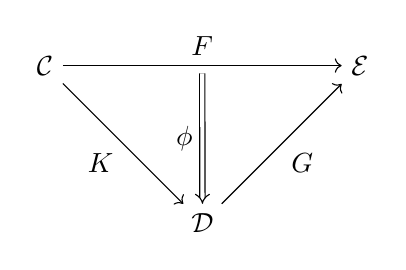
\begin{tikzpicture}
            \node (C) at (-2,2) {\(\mathcal{C}\)};
            \node (D) at (0,0) {\(\mathcal{D}\)};
            \node (E) at (2,2) {\(\mathcal{E}\)};
            \draw[->] (C) to node[above] (F) {\(F\)} (E);
            \draw[->] (C) to node[below left] {\(K\)} (D);
            \draw[->] (D) to node[below right] (G) {\(G\)} (E);
            \draw[-{Implies},double,double distance = 0.15em] ($(F.south) + (0 , - 0.1)$) to node[left] {\(\phi\)} (D);
        \end{tikzpicture}
    \]

    对偶的, 定义右 Kan 延拓 \(\mathrm{Ran}_K F : \mathcal{D} \to \mathcal{E}\) 与其对应的 \(2\) - 态射 \(\varepsilon : \mathrm{Ran}_K F \circ K \to F\),
    满足任给 \(G : \mathcal{D} \to \mathcal{E}\) 与 \(2\) - 态射 \(\phi : G \circ K \to F\), 存在唯一的 \(2\) - 态射 \(\phi^\prime : G \to \mathrm{Ran}_K F\), 满足以下等式:

    \[
        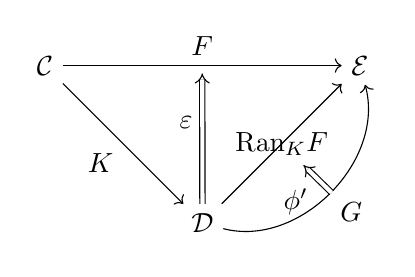
\begin{tikzpicture}
            \node (C) at (-2,2) {\(\mathcal{C}\)};
            \node (D) at (0,0) {\(\mathcal{D}\)};
            \node (E) at (2,2) {\(\mathcal{E}\)};
            \draw[->] (C) to node[above] (F) {\(F\)} (E);
            \draw[->] (C) to node[below left] {\(K\)} (D);
            \draw[->] (D) to [bend right = 60] node[below right] (G) {\(G\)} (E);
            \draw[->] (D) to node (Ran) {\(\mathrm{Ran}_K F\)} (E);
            \draw[-{Implies},double,double distance = 0.15em] (D) to node[above left] {\(\varepsilon\)} ($(F.south) + (0 , - 0.1)$);
            \draw[-{Implies},double,double distance = 0.15em] (G) to node[below left] {\(\phi^\prime\)} (Ran);
        \end{tikzpicture} = 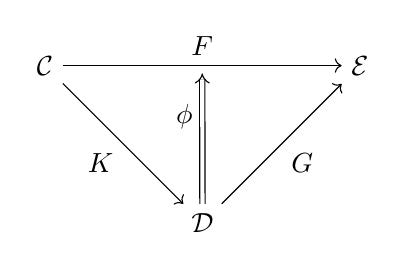
\begin{tikzpicture}
            \node (C) at (-2,2) {\(\mathcal{C}\)};
            \node (D) at (0,0) {\(\mathcal{D}\)};
            \node (E) at (2,2) {\(\mathcal{E}\)};
            \draw[->] (C) to node[above] (F) {\(F\)} (E);
            \draw[->] (C) to node[below left] {\(K\)} (D);
            \draw[->] (D) to node[below right] (G) {\(G\)} (E);
            \draw[-{Implies},double,double distance = 0.15em] (D) to node[above left] {\(\phi\)} ($(F.south) + (0 , - 0.1)$);
        \end{tikzpicture}
    \]
\end{definition}

\begin{lemma}
    Kan 延拓存在则在同构意义下唯一.

    \begin{proof}
        利用泛性质唯一性.
    \end{proof}
\end{lemma}

\begin{lemma}
    如若所有 \(F : \mathcal{C} \to \mathcal{E}\) 的右 Kan 延拓存在, 则 \(\mathrm{Ran}_K\) 给出
    从 \(\mathrm{Hom} (\mathcal{C}, \mathcal{E})\) 到 \(\mathrm{Hom} (\mathcal{D}, \mathcal{E})\) 的函子.

    \begin{proof}
        需给出 \(\mathrm{Ran}_K\) 对态射的作用, 给出 \(F \to G\) 的态射 \(\phi : F \to G\), 定义 \(\mathrm{Ran}_K \phi\) 为使得以下等式成立的唯一态射:

        \[
            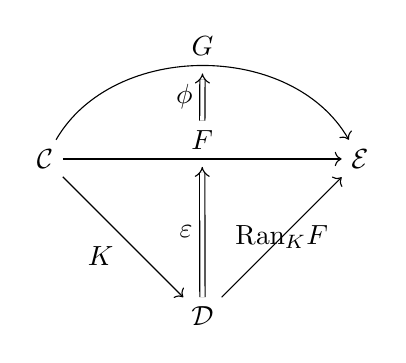
\begin{tikzpicture}
                \node (C) at (-2,2) {\(\mathcal{C}\)};
                \node (D) at (0,0) {\(\mathcal{D}\)};
                \node (E) at (2,2) {\(\mathcal{E}\)};
                \draw[->] (C) to node[above] (F) {\(F\)} (E);
                \draw[->] (C) to [bend left = 60] node[above] (G) {\(G\)} (E);
                \draw[->] (C) to node[below left] {\(K\)} (D);
                \draw[->] (D) to node (Ran) {\(\mathrm{Ran}_K F\)} (E);
                \draw[-{Implies},double,double distance = 0.15em] (D) to node[left] {\(\varepsilon\)} ($(F.south) + (0 , - 0.1)$);
                \draw[-{Implies},double,double distance = 0.15em] (F) to node[left] {\(\phi\)} ($(G.south) + (0 , - 0.1)$);
            \end{tikzpicture} = 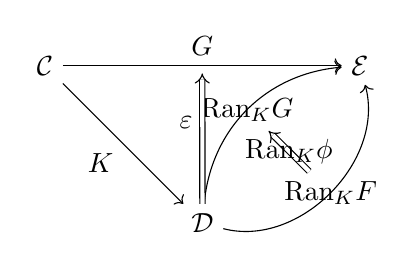
\begin{tikzpicture}
                \node (C) at (-2,2) {\(\mathcal{C}\)};
                \node (D) at (0,0) {\(\mathcal{D}\)};
                \node (E) at (2,2) {\(\mathcal{E}\)};
                \draw[->] (C) to node[above] (G) {\(G\)} (E);
                \draw[->] (C) to node[below left] {\(K\)} (D);
                \draw[->] (D) to [bend left = 40] node (RanG) {\(\mathrm{Ran}_K G\)} (E);
                \draw[->] (D) to [bend right = 60] node (RanF) {\(\mathrm{Ran}_K F\)} (E);
                \draw[-{Implies},double,double distance = 0.15em] (RanF) to node {\(\mathrm{Ran}_K \phi\)} (RanG);
                \draw[-{Implies},double,double distance = 0.15em] (D) to node[above left] {\(\varepsilon\)} ($(G.south) + (0 , - 0.1)$);
            \end{tikzpicture}
        \]

        函子性由唯一性保证.
    \end{proof}
\end{lemma}

\begin{corollary}
    同理, 假定对于所有 \(F : \mathcal{C} \to \mathcal{E}\) 的左 Kan 延拓存在, 则 \(\mathrm{Lan}_K\) 也给出
    从 \(\mathrm{Hom} (\mathcal{C}, \mathcal{E})\) 到 \(\mathrm{Hom} (\mathcal{D}, \mathcal{E})\) 的函子.
\end{corollary}

\begin{lemma}
    有伴随对 \(\mathrm{Lan}_K \dashv (- \circ K) \dashv \mathrm{Ran}_K\), 其中 \((- \circ K)\) 
    定义为将 \(1\) - 态射合成 \(K\), 而将 \(2\) - 态射横合成 \(\mathrm{id}_K\).

    \begin{proof}
        态射集 \(\mathrm{Hom}_{\mathrm{Hom} (\mathcal{D}, \mathcal{E})} (\mathrm{Lan}_K (F),G) \to \mathrm{Hom}_{\mathrm{Hom} (\mathcal{C}, \mathcal{E})} (F,G \circ K)\)
        无非是定义的复写. 在 \(F\) 处自然性是按 \(\mathrm{Lan}_K\) 对态射变换的定义, 在  \(G\) 处的自然性依赖唯一性.
    \end{proof}
\end{lemma}

\begin{lemma}
    在 \(\mathbf{Cat}\) 中考虑, 伴随对 \(F \dashv G\) 给出 Kan 延拓 \(G = \mathrm{Lan}_F (\mathrm{id}_\mathcal{C})\), \(F = \mathrm{Ran}_G (\mathrm{id}_\mathcal{C})\).

    \begin{proof}
        观察下图的合成

        \begin{center}
            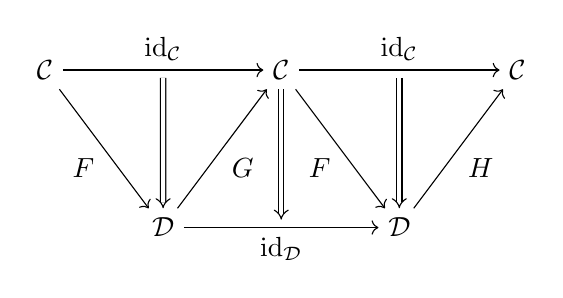
\begin{tikzpicture}
                \node (C1) at (-3,1) {\(\mathcal{C}\)};
                \node (C2) at (0,1) {\(\mathcal{C}\)};
                \node (C3) at (3,1) {\(\mathcal{C}\)};
                \node (D1) at (-1.5,-1) {\(\mathcal{D}\)};
                \node (D2) at (1.5,-1) {\(\mathcal{D}\)};
                \draw[->] (C1) to node[above] (idc1) {\(\mathrm{id}_{\mathcal{C}}\)} (C2);
                \draw[->] (C2) to node[above] (idc2) {\(\mathrm{id}_{\mathcal{C}}\)} (C3);
                \draw[->] (D1) to node[below] (idd) {\(\mathrm{id}_{\mathcal{D}}\)} (D2);
                \draw[->] (C1) to node[below left] {\(F\)} (D1);
                \draw[->] (C2) to node[below left] {\(F\)} (D2);
                \draw[->] (D1) to node[below right] {\(G\)} (C2);
                \draw[->] (D2) to node[below right] {\(H\)} (C3);
                \draw[-{Implies},double,double distance = 0.15em] ($(idc1.south) + (0,-0.1)$) to (D1);
                \draw[-{Implies},double,double distance = 0.15em] (C2) to ($(idd.north) + (0,0.1)$);
                \draw[-{Implies},double,double distance = 0.15em] ($(idc2.south) + (0,-0.1)$) to (D2);
            \end{tikzpicture}
        \end{center}

        所需 \(2\) 态射为右侧平行四边形, 另一个方向亦然.
    \end{proof}
\end{lemma}

\subsection{极限}

定义 \(\mathbf{1}\) 为最简单的范畴, 仅有一个对象与一个态射, 记为 \(\bullet\), 任何
范畴都有唯一的函子 \(\mathbf{1} \to \mathcal{C}\).

\begin{definition}[极限]
    在范畴 \(\mathbf{Cat}\) 中考虑.
    
    给出小范畴 \(I\) 与函子 \(F : I \to \mathcal{C}\), \(K : I \to \mathbf{1}\), 
    若 \(\mathrm{Ran}_K F\) 存在, 则称 \(\mathrm{Ran}_K F\) 为 \(F\) 的极限 (limit), 记为 \(\varprojlim F\),
    对称的 \(\mathrm{Lan}_K F\) 称为 \(F\) 的余极限 (colimit), 记为 \(\varinjlim F\), 称 \(I^\mathrm{op}\) 为极限对应的指标, \(I\) 为余极限对应的指标.
\end{definition}

解释一下上述对于极限的定义, 给出一个 \(\mathbf{1}\) 出发的函子, 即选中了 \(\mathcal{C}\) 中的一个对象 (此对象沿用上述符号记作 \(\varprojlim F\) 或 \(\varinjlim F\)),
极限构造中上述 Kan 延拓给出的自然变换标记了从该对象出发的函子到 \(F I\) 中一对象的态射, 满足对于任意 \(f \in \mathrm{Mor}(I)\), 下图交换:

\begin{center}
    \begin{tikzpicture}
        \node (FX) at (-2,2) {\(F X\)};
        \node (FY) at (2,2) {\(F Y\)};
        \node (lim) at (0,0) {\(\varprojlim F\)};
        \draw[->] (FX) to node[above] (Ff) {\(F f\)} (FY);
        \draw[->] (lim) to (FX);
        \draw[->] (lim) to (FY);
    \end{tikzpicture}
\end{center}

Kan 延拓的性质也就被解为, 对于任意给出的 \(L \in \mathcal{C}\), 一族态射 \(\phi_X : L \to F X\), 使得对于任意 \(f \in \mathrm{Mor}(I)\), 下图交换:

\begin{center}
    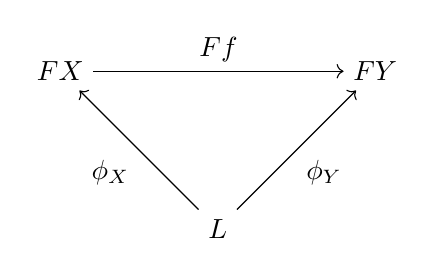
\begin{tikzpicture}
        \node (FX) at (-2,2) {\(F X\)};
        \node (FY) at (2,2) {\(F Y\)};
        \node (L) at (0,0) {\(L\)};
        \draw[->] (FX) to node[above] (Ff) {\(F f\)} (FY);
        \draw[->] (L) to node[below left] (phiX) {\(\phi_X\)} (FX);
        \draw[->] (L) to node[below right] (phiY) {\(\phi_Y\)} (FY);
    \end{tikzpicture}
\end{center}

都有唯一的态射 \(\phi_f : L \to \varprojlim F\), 使得对于任意 \(X \in \mathrm{Ob} (I)\) 下图交换:

\begin{center}
    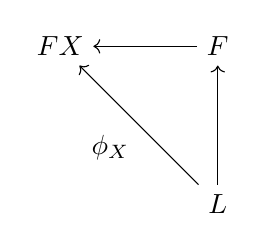
\begin{tikzpicture}
        \node (FX) at (-2,2) {\(F X\)};
        \node (L) at (0,0) {\(L\)};
        \node (lim) at (0,2) {\(\varprojlim F\)};
        \draw[->] (lim) to (FX);
        \draw[->] (L) to node[below left] (phiX) {\(\phi_X\)} (FX);
        \draw[->] (L) to (lim);
    \end{tikzpicture}
\end{center}

余极限将上述所有箭头反向即可得到.

\begin{definition}
    直积 (product) 与余积 (coproduct) 是极限与余极限的特例, 分别对应于 \(I\) 为离散范畴的极限与余极限.
\end{definition}

\begin{example}
    \(\mathbf{Set}\) 中直积为笛卡尔积, 余积为不交并.
\end{example}

\begin{definition}
    等化子 (equalizer) 与余等化子 (coequalizer) 是极限与余极限的特例, 分别对应于 \(I\) 为下图所示的范畴的极限与余极限 (\(\mathrm{id}\) 未画出).

    \begin{center}
        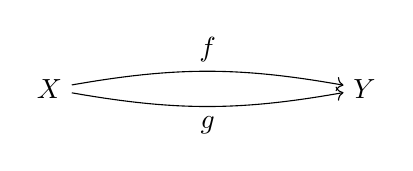
\begin{tikzpicture}
            \node (X) at (-2,0) {\(X\)};
            \node (Y) at (2,0) {\(Y\)};
            \draw[->] (X) to [bend left = 10] node[above] (f) {\(f\)} (Y);
            \draw[->] (X) to [bend right = 10] node[below] (g) {\(g\)} (Y);
        \end{tikzpicture}
    \end{center}
\end{definition}

\begin{lemma}
    \label {lemma:existence of limitation of homeomorphism}
    给出自然变换 \(\psi : \alpha \to \alpha^\prime\), 假使极限存在则存在唯一 \(\psi\) 使对任意 \(i\) 以下图表交换:

    \begin{center}
        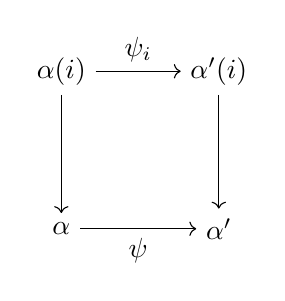
\begin{tikzpicture}
            \node (ai) at (-1,1) {\(\alpha (i)\)};
            \node (api) at (1,1) {\(\alpha^\prime (i)\)};
            \node (lima) at (-1,-1) {\(\varinjlim \alpha\)};
            \node (limap) at (1,-1) {\(\varinjlim \alpha^\prime\)};
            \draw[->] (ai) to node[above] (aii) {\(\psi_i\)} (api);
            \draw[->] (ai) to (lima);
            \draw[->] (api) to (limap);
            \draw[->] (lima) to node[below] (limf) {\(\varinjlim \psi\)} (limap);
        \end{tikzpicture}
    \end{center}

    \begin{proof}
        态射合成给出了 \(\alpha(i) \to \varinjlim \alpha^\prime\), 其与 \(\mathrm{Mor}(I)\) 相容, 由极限的定义唯一性给出了 \(\varinjlim \alpha \to \varinjlim \alpha^\prime\).
    \end{proof}
\end{lemma}

\begin{corollary}
    给出自然变换 \(\psi : \alpha \to \alpha^\prime\), 假使极限存在则存在唯一 \(\psi\) 使对任意 \(i\) 以下图表交换:

    \begin{center}
        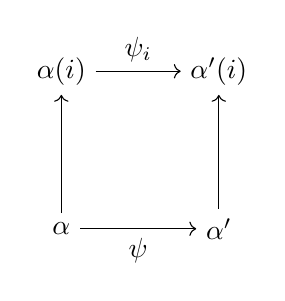
\begin{tikzpicture}
            \node (ai) at (-1,1) {\(\alpha (i)\)};
            \node (api) at (1,1) {\(\alpha^\prime (i)\)};
            \node (lima) at (-1,-1) {\(\varprojlim \alpha\)};
            \node (limap) at (1,-1) {\(\varprojlim \alpha^\prime\)};
            \draw[->] (ai) to node[above] (aii) {\(\psi_i\)} (api);
            \draw[->] (lima) to (ai);
            \draw[->] (limap) to (api);
            \draw[->] (lima) to node[below] (limf) {\(\varprojlim \psi\)} (limap);
        \end{tikzpicture}
    \end{center}
\end{corollary}

\begin{lemma}
    给出自然变换 \(\psi : \alpha_1 \to \alpha_2\),  \(\phi : \alpha_2 \to \alpha_3\), 假使极限存在则有等式 \(\varinjlim (\phi \psi) = \varinjlim \phi \varinjlim \psi\).

    \begin{proof}
            无非是交换图表:

            \begin{center}
                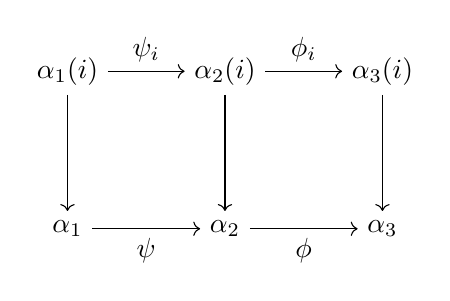
\begin{tikzpicture}
                    \node (a1i) at (-2,1) {\(\alpha_1 (i)\)};
                    \node (a2i) at (0,1) {\(\alpha_2 (i)\)};
                    \node (a3i) at (2,1) {\(\alpha_3 (i)\)};
                    \node (lima1) at (-2,-1) {\(\varinjlim \alpha_1\)};
                    \node (lima2) at (0,-1) {\(\varinjlim \alpha_2\)};
                    \node (lima3) at (2,-1) {\(\varinjlim \alpha_3\)};
                    \draw[->] (a1i) to node[above] (psi) {\(\psi_i\)} (a2i);
                    \draw[->] (a2i) to node[above] (phi) {\(\phi_i\)} (a3i);
                    \draw[->] (a1i) to (lima1);
                    \draw[->] (a2i) to (lima2);
                    \draw[->] (a3i) to (lima3);
                    \draw[->] (lima1) to node[below] (limpsi) {\(\varinjlim \psi\)} (lima2);
                    \draw[->] (lima2) to node[below] (limphi) {\(\varinjlim \phi\)} (lima3);
                \end{tikzpicture}
            \end{center}
    \end{proof}
\end{lemma}

\begin{corollary}
    同理有等式 \(\varprojlim (\phi \psi) = \varprojlim \phi \varprojlim \psi\).
\end{corollary}

\begin{lemma}
    直积的直积 (余积的余积) 为直积 (余积).

    \begin{proof}
        给出对象 \(X_{i,j}\) 的直积 \(X_{i} := \prod_j X_{i,j}\) 与直积 \(X := \prod_i X_i\),
        无非是说对于任意对象 \(Y\), \(\prod_{i,j} \mathrm{Hom} (Y,X_{i,j})\) 与 \(\prod_i \mathrm{Hom} (Y,X_i)\), \(\mathrm{Hom} (Y,X)\) 一一对应,
        老直积态射的合成给出新直积所需的态射.
    \end{proof}
\end{lemma}

\begin{definition}
    考察以下范畴 \(I\):

    \begin{center}
        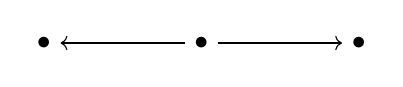
\begin{tikzpicture}
            \node (B1) at (-2,0) {\(\bullet\)};
            \node (B2) at (0,0) {\(\bullet\)};
            \node (B3) at (2,0) {\(\bullet\)};
            \draw[->] (B2) to (B1);
            \draw[->] (B2) to (B3);
        \end{tikzpicture}
    \end{center}

    以 \(I\) 为指标的极限称纤维积 (fibre product) 或拉回 (pullback), \(I\) 的余极限称纤维余积或推出 (pushout), 记作 Cartesius 图表:

    \begin{center}
        \begin{tikzpicture}
            \node (prod) at (-1,1) {\(X \times_Z Y\)};
            \node (X) at (1,1) {\(X\)};
            \node (Y) at (-1,-1) {\(Y\)};
            \node (Z) at (1,-1) {\(Z\)};
            \draw[->] (X) to (Z);
            \draw[->] (Y) to (Z);
            \draw[->] (prod) to (X);
            \draw[->] (prod) to (Y);
            \node at (0,0) {\(\Box\)};
        \end{tikzpicture} \begin{tikzpicture}
            \node (coprod) at (-1,1) {\(X \sqcup_Z Y\)};
            \node (X) at (1,1) {\(X\)};
            \node (Y) at (-1,-1) {\(Y\)};
            \node (Z) at (1,-1) {\(Z\)};
            \draw[->] (Z) to (X);
            \draw[->] (Z) to (Y);
            \draw[->] (X) to (coprod);
            \draw[->] (Y) to (coprod);
            \node at (0,0) {\(\boxplus\)};
        \end{tikzpicture}
    \end{center}
\end{definition}

\begin{definition}
    若范畴 \(\mathcal{C}\) 满足所有以某个小范畴为指标的 \(\varprojlim\) 存在
    则 \(\mathcal{C}\) 是完备的, 对称的 \(\varinjlim\) 存在则 \(\mathcal{C}\) 是余完备的.
\end{definition}

\begin{lemma}
    对于完备的范畴 \(\mathcal{C}\), \(\varinjlim\) 与 \(\varprojlim\) 给出了 \(\mathbf{Fun} (I,\mathcal{C})\) 到 \(\mathcal{C}\) 的函子.
\end{lemma}

\begin{definition}
    定义拟序集 \(P\) 的范畴, 其对象为 \(P\) 中的元素, 在 \(X \leq Y\) 时 \(\abs{\mathrm{Hom} (X,Y)} = 1\) 的范畴.
\end{definition}

\begin{lemma}[Freyd]
    小范畴 \(\mathcal{C}\) 完备当且仅当 \(\mathcal{C}\) 从某个拟序集 \(P\) 构造出来, 且 \(P\) 中每个子集都有下确界.

    \begin{proof}
        假定有 \(f,g : X \to Y\), 则 \(\abs{\mathrm{Hom} (X,Y^{\abs{\mathrm{Mor} (\mathcal{C})}})} > \mathrm{Mor} (\mathcal{C})\)
        矛盾, 此时极限就是下确界.
    \end{proof}
\end{lemma}

\begin{theorem}
    假使范畴 \(\mathcal{C}\) 含所有直积与等化子, 则 \(\mathcal{C}\) 是完备的.

    \begin{proof}
        给出小范畴 \(I\) 与函子 \(F : I \to \mathcal{C}\), 令 \(X := \prod_{i \in \mathrm{Ob} (I)} F i\),
        \(Y := \prod_{\sigma \in \mathrm{Mor} (\mathcal{C})} F (t (\sigma))\), \(Z := \prod_{\sigma \in \mathrm{Mor} (\mathcal{C})} F (s (\sigma))\),
        考察 \(X \to Y\) 的两个态射, 一个逐点, 一个逐点透过 \(Z\), 然后透过 \(\sigma\), 其等化子自然与 \(\sigma\) 相容, 即为极限.
    \end{proof}
\end{theorem}

\begin{corollary}
    假使范畴 \(\mathcal{C}\) 含所有余积与余等化子, 则 \(\mathcal{C}\) 是余完备的.
\end{corollary}

\begin{lemma}
    \(\mathbf{Set}\) 是完备的.

    \begin{proof}
        显然 \(\mathbf{Set}\) 含所有直积, 余积, 等化子, 余等化子.
    \end{proof}
\end{lemma}

\begin{definition}[滤过]
    \setlabel {滤过}
    \label {definition:filtered category}
    给出小范畴 \(I\), 若任取 \(i,j \in \mathrm{Ob} (I)\), 存在 \(k \in \mathrm{Ob} (I)\), 使得 \(i,j\) 到 \(k\) 有态射,
    且对于任意 \(f,g : i \to j\), 存在 \(h : j \to k\), 使得 \(h f = h g\), 则称 \(I\) 滤过 (filtered).
\end{definition}

滤过的好处在于允许我们显式地在某些特定的范畴 (如 \(\mathbf(Set)\)) 中构造余极限, 因为此处等化子是可以直接写出来的等价关系.

\begin{lemma}
    \(\mathcal{C}^{\wedge}\) 与 \(\mathcal{C}^{\vee}\) 是完备且余完备的.

    \begin{proof}
        只需给 \(\mathcal{C}\) 中每一个点赋予极限与余极限, 利用 \ref {lemma:existence of limitation of homeomorphism} 即可.
    \end{proof}
\end{lemma}

这里要注意到嵌入的过程, 假若嵌入 \(\mathbf{Set}^\mathrm{op}\), 而在 \(\mathbf{Set}\) 中考虑对应极限, 需转换 \(\lim\) 方向.

\begin{lemma}
    \label {lemma:existence of limit iff representable}
    函子 \(\alpha : I \to \mathcal{C}\) 余极限存在当且仅当米田嵌入之后的余极限可表, 极限亦然.

    \begin{proof}
        米田嵌入给出的 \(\mathrm{Hom}\) 集的对应无非就是极限的定义.
    \end{proof}
\end{lemma}

\begin{definition}
    极限存在时, 称函子 \(F\) 保 \(\varprojlim \alpha\), 如果 \(F \varprojlim \alpha \simeq \varprojlim F \alpha\), 亦定义保 \(\varinjlim \alpha\).
\end{definition}

\begin{corollary}
    取 \(X \in \mathcal{C}\), 则函子 \(\mathrm{Hom} (X,-)\) 保 \(\varprojlim\), \(\mathrm{Hom} (-,X)\) 保 \(\varinjlim\).
\end{corollary}

\begin{theorem}
    若 \(F \dashv G\), 则 \(F\) 保 \(\varinjlim\), \(G\) 保 \(\varprojlim\).

    \begin{proof}
        考察 \(\mathcal{C}^{\vee}\) 中的等式:

        \[
            \begin{aligned}
                \mathrm{Hom}_{\mathcal{D}} (F \varinjlim \alpha, -) & \simeq \mathrm{Hom}_\mathcal{C} (\varinjlim \alpha, G (-)) \\
                & \simeq \varinjlim \mathrm{Hom}_\mathcal{C} (\alpha (i), G (-)) \\
                & \simeq \varinjlim \mathrm{Hom}_\mathcal{D} (F \alpha (i), -) \\
                & \simeq \mathrm{Hom}_\mathcal{D} (\varinjlim F \alpha, -)
            \end{aligned}
        \]

        依米田嵌入全忠实性, 此给出二者之同构.
    \end{proof}
\end{theorem}

    \section{点集拓扑}

\subsection{基础定义}

拓扑是用来度量连续性的.

\begin{definition}[拓扑空间]
    拓扑空间 (topological space) 指资料 \((X,\mathcal{T})\) 使得 \(X\) 是集合且 \(\mathcal{T} \subseteq \mathcal{P}(X)\), 并满足:
    \begin{enumerate}
        \item \(\emptyset, X \in \mathcal{T}\)
        \item 有限交 (finite intersection) \(\forall A_1, \dots, A_n \in \mathcal{T} (\bigcap_{i=1}^n A_i \in \mathcal{T})\)
        \item 任意并 (arbitrary union) \(\forall \mathcal{A} \subseteq \mathcal{T} (\bigcup_{A \in \mathcal{A}} A \in \mathcal{T})\)
    \end{enumerate}
    称 \(\mathcal{T}\) 中的元素为开集.
\end{definition}

\begin{definition}
    对于任何集合 \(X\), 分别取 \(\mathcal{T} = \mathcal{P} (X)\) 与 \(\mathcal{T} = \{\varnothing,X\}\) 可得到两个拓扑
    分别称离散拓扑 (discrete topology) 与凝聚拓扑 (indiscrete topology).
\end{definition}

\begin{definition}
    假定 \(X\) 上有两个拓扑 \(\mathcal{T}\) 与 \(\mathcal{T}^\prime\), 如果 \(\mathcal{T} \subseteq \mathcal{T}^\prime\), 则称 \(\mathcal{T}^\prime\) 比 \(\mathcal{T}\) 细 (finer),
    反之如果 \(\mathcal{T}^\prime \subseteq \mathcal{T}\), 则称 \(\mathcal{T}^\prime\) 比 \(\mathcal{T}\) 粗 (coarser).
\end{definition}

\begin{lemma}
    对 \(X\) 上拓扑 \({(\mathcal{T}_i)}_{i \in I}\) 的交 \(\bigcap_{i \in I} \mathcal{T}_i\) 是拓扑.
\end{lemma}

\begin{definition}[拓扑基]
    给定 \(X\) 与 \(\mathcal{B} \subseteq \mathcal{P}(X)\), 如果 \(\mathcal{B}\) 满足:
    \begin{enumerate}
        \item \(\forall x \in X \exists B \in \mathcal{B} (x \in B)\)
        \item 对任意 \(x,A,B\) 假使 \(x \in A \cap B\) 且 \(A,B \in \mathcal{B}\), 则存在 \(C \in \mathcal{B}\) 使得 \(x \in C \subseteq A \cap B\)
    \end{enumerate}
    则称 \(\mathcal{B}\) 为 \(X\) 上的拓扑基 (topological base).
\end{definition}

\begin{definition}
    如果 \(\mathcal{T}\) 是包含 \(\mathcal{B}\) 的最粗拓扑, 则称 \(\mathcal{B}\) 为 \(\mathcal{T}\) 的拓扑基.
\end{definition}

\begin{lemma}
    一个集合 \(U \subseteq X\) 在 \(\mathcal{B}\) 生成的拓扑中开当且仅当 \(\forall x \in U : \exists B_x \in \mathcal{B} (x \in B_x \subseteq U)\).

    \begin{proof}
        这些集合 \(U\) 总是开, 因为 \(U = \bigcup_{x \in U} B_x\).

        这些集合构成拓扑, 只需逐条验证:
        \begin{enumerate}
            \item \(\neg (\exists x \in \varnothing)\) 且 \(\forall x \exists B \in \mathcal{B} (x \in B)\), 故 \(\varnothing, X\) 开.
            \item 任意给出集合 \(U,V\) 开, 则只需注意到 \(x \in B_x \subseteq B_x^U \cap B_x^V \subseteq U \cap V\), 故 \(U \cap V\) 仍开, 有限交无非是二元情况下的延伸.
            \item 任意给出 \({(U_i)}_{i \in I}\), 只需取 \(B_x\) 为某个 \(U_i\) 中 \(x\) 对应的 \(B_x\) 即可.
        \end{enumerate}
    \end{proof}
\end{lemma}

\begin{definition}
    对 \(x \in X\), 称 \(x \in B_x \in \mathcal{B}\) 为基本邻域, 称 \(x \in U \in \mathcal{T}\) 为邻域,
    全体 \(x\) 邻域记作 \(\mathcal{T}_x\).
\end{definition}

\begin{definition}
    \label {definition:topological space's category}
    对于拓扑空间 \((X,\mathcal{T})\), 定义其对应的范畴 \(\mathrm{Cat} (\mathcal{T})\) 如下:

    \begin{enumerate}
        \item 对象是 \(\mathcal{T}\) 中的元素.
        \item \(X \subseteq Y\) 时有唯一态射 \(X \to Y\).
        \item \(X \nsubseteq Y\) 时没有态射.
    \end{enumerate}
\end{definition}

\begin{definition}
    对于拓扑空间 \((X,\mathcal{T}_x), (Y,\mathcal{T}_y)\) 与映射 \(f : X \to Y\),
    如果 \(\forall U \in \mathcal{T}_Y (f^{-1} (U) \in \mathcal{T}_X)\), 则称 \(f\) 连续 (continuous).
\end{definition}

\begin{lemma}
    连续映射的复合仍然连续.

    \begin{proof}
        对于连续映射 \(f : X \to Y, g : Y \to Z\), 有 \(\forall U \in \mathcal{T}_Z (g^{-1} (U) \in \mathcal{T}_Y)\) 且 \(\forall V \in \mathcal{T}_Y (f^{-1} (V) \in \mathcal{T}_X)\),
    \end{proof}
\end{lemma}

\begin{corollary}
    连续映射 \(f : X \to Y\) 诱导出函子 \(\mathrm{Cat} (\mathcal{T}_y) \to \mathrm{Cat} (\mathcal{T}_x)\).
\end{corollary}

\begin{definition}
    定义拓扑空间范畴 \(\mathbf{Top}\) 如下:
    \begin{enumerate}
        \item 对象是拓扑空间.
        \item \(\mathbf{Hom}_{\mathbf{Top}} (X,Y)\) 是所有连续映射 \(f : X \to Y\).
    \end{enumerate}
\end{definition}

\begin{corollary}
    上述定义的 \(\mathrm{Cat}\) 给出 \(\mathbf{Top} \to \mathbf{Cat}\) 的一个反变函子.
\end{corollary}

\begin{definition}
    一个度量空间是包含资料 \((X,d)\) 使得 \(X\) 是集合且 \(d : X \times X \to \mathbb{R}\) 满足:
    \begin{enumerate}
        \item \(d(x,y) \geq 0\)
        \item \(d(x,y) = 0 \iff x = y\)
        \item \(d(x,y) = d(y,x)\)
        \item \(d(x,z) \leq d(x,y) + d(y,z)\)
    \end{enumerate}
\end{definition}

\begin{example}
    取 \(\mathbb{R}\) 上 \(d(x,y) = \abs{x - y}\) 可得到度量空间.
\end{example}

\begin{example}
    取 \(\mathbb{R}^n\) 上 \(d(x,y) = \max \{\abs{x_i - y_i}\}\) 可得到度量空间.
\end{example}


    \include{Foundations/monoidalcategory.tex}

    \chapter{代数基础}
    \chapter{分析基础}
    \chapter{代数拓扑}
    \section{基本群}


    \chapter{代数数论}



    % \printindex
    \printbibliography[heading=bibintoc]


\end{document}